% Geometric Dark Energy from Spin-Torsion Cosmology
% Houston Golden — 2026
% arXiv submission: gr-qc / astro-ph.CO / hep-th
%
% Compile: pdflatex main && bibtex main && pdflatex main && pdflatex main

\documentclass[aps,prd,twocolumn,superscriptaddress,showpacs,preprintnumbers,nofootinbib,longbibliography,floatfix]{revtex4-2}

\usepackage{amsmath,amssymb,amsfonts}
\usepackage{graphicx}
\usepackage{bm}
\usepackage{hyperref}
\usepackage{xcolor}
\usepackage{booktabs}
\usepackage{multirow}
\usepackage{dcolumn}
\usepackage{enumitem}
\usepackage{mathtools}
\usepackage{bbold}
\usepackage[utf8]{inputenc}
\usepackage{float}
\usepackage{slashed}

\hypersetup{
  colorlinks=true,
  linkcolor=blue!60!black,
  citecolor=blue!60!black,
  urlcolor=blue!60!black
}

% Custom commands
\newcommand{\Leff}{\Lambda_{\rm eff}}
\newcommand{\Lconst}{\Lambda_{\rm const}}
\newcommand{\Lobs}{\Lambda_{\rm obs}}
\newcommand{\Dinf}{\mathcal{D}_{\rm inf}}
\newcommand{\rhocrit}{\rho_{\rm crit}}
\newcommand{\rhoPl}{\rho_{\rm Pl}}
\newcommand{\MPl}{M_{\rm Pl}}
\newcommand{\Neff}{N_{\rm eff}}
\newcommand{\ie}{i.e.}
\newcommand{\eg}{e.g.}
\newcommand{\cf}{cf.}
\newcommand{\etal}{\textit{et~al.}}
\newcommand{\fnl}{f_{\rm NL}}
\newcommand{\fcw}{f_{\rm CW}}
\newcommand{\paperVersion}{v2.3.17}
\newcommand{\paperTimestamp}{2026-05-04 11:00 PDT}

\begin{document}

\preprint{HUBIFY-2026-001}

\title{Structural Closure of Einstein--Cartan--Holst Dark Energy:\\
Perturbation Transparency, Inflation--$f_{\rm NL}$ Tension, and Surviving Matter-Bounce Tests}

\author{Houston Golden}
\email{houston@hubify.com}
\affiliation{Independent Researcher, Los Angeles, California, USA}

\date{May 4, 2026, 11:00 PDT --- \paperVersion}

\begin{abstract}
We investigate whether Einstein-Cartan-Holst (ECH) spin-torsion gravity can produce late-time dark energy or distinctive cosmological signatures. LQC holonomy corrections yield a nonsingular quantum bounce at $\rho_{\rm crit} \approx 0.27$--$0.41\,\rho_{\rm Pl}$, while the ECH parity structure generates a unique four-fermion interaction. Through 7 foundation studies and 17 research branches we establish 14 independent structural constraints that map which minimal routes from the bounce to late-time dark energy survive observational testing within ECH. A perturbation-transparency observation (generalizing Hehl 1976~\cite{Hehl1976}) shows that for canonical scalar matter, torsion vanishes at all perturbation orders and the Holst dual contraction $\epsilon^{\mu\nu\rho\sigma}R_{\mu\nu\rho\sigma}$ vanishes identically by the first Bianchi identity, establishing that the Holst sector decouples from all scalar/tensor perturbation observables and identifying the nonperturbative parity-violating channels (ALP birefringence, primordial gravitational waves) as the relevant tests of the Barbero--Immirzi parameter $\gamma$. The proposed link from ECH to a late-time vacuum energy goes through a phenomenological dimensional ansatz $\rho_\Lambda = \Xi\,M_{\rm Pl}^4$ (Sec.~\ref{sec:parityodd}, Appendix~\ref{app:dimensions}), which is dimensionally correct on-shell at the bounce but is \emph{not} an EFT derivation from the ECH action; the Holst sector and the late-time $\rho_\Lambda$ are connected only by this ansatz. A stock-CAMB $\Lambda$CDM$+\Delta\Neff$ MCMC (Cobaya~v3.6.1, 424{,}781 samples across three dataset combinations; see Sec.~\ref{sec:verification}) is reported as a \emph{$\Lambda$CDM$+\Delta\Neff$ proxy} only---the Boltzmann code carries zero spin-torsion modifications, so this run does \emph{not} test the ECH theory module---and finds $\Delta\Neff$ consistent with zero and $H_0 = 67.68\pm 1.06\,\text{km}\,\text{s}^{-1}\,\text{Mpc}^{-1}$, recovering $\Lambda$CDM. The primary model-comparison cross-reference for this proxy (Sec.~\ref{sec:cosmo_fits}) is $\Delta\text{AIC} = -5.9$ (mild evidence for $\Lambda$CDM$+\Delta\Neff$ on Akaike grounds) and $\Delta\text{BIC} = -0.7$ (below the conventional $|\Delta\text{BIC}|=2$ detection threshold); the biased Savage-Dickey estimate $\ln B = +4.8$ is demoted to a footnote because the $r=-0.89$ correlation between $\Delta\Neff$ and $H_0$ significantly biases that estimator and the model refers to $\Lambda$CDM$+\Delta\Neff$, not to the spin-torsion theory. The actual statistical detection significance of cosmic birefringence is the published Planck/ACT~DR6 $2.4$--$2.9\sigma$ (a methodology pipeline-recovery cross-check using NaMaster pseudo-$C_\ell$ on the Planck Commander map is reported as a cross-check in Sec.~\ref{sec:data_cmb} only and is \emph{not} part of the observational evidence reported in this abstract or in Table~\ref{tab:summary}). Phenomenological dark-energy connection requires assumptions beyond the minimal framework, and perturbation observables decouple cleanly from the Holst sector. An open structural question (Sec.~\ref{sec:structural_tension}) is the incompatibility between the inflationary-suppression dark-energy mechanism, which requires $N_{\rm tot} \approx 92$ $e$-folds of post-bounce inflation, and the matter-bounce $f_{\rm NL}$ signature, which would be erased by that many $e$-folds; consistent with this, we treat bounce cosmology and dark energy as independent observational problems. The surviving testable observable is from the matter-bounce class~\cite{Cai:2009fn} (of which ECH is one possible UV completion; the $f_{\rm NL}$ value is shared by every dust-dominated contracting bounce and is \emph{not} a distinctive ECH prediction): $f_{\rm NL} = -35/8$, consistent with the matter-bounce scenario and testable by SPHEREx at $3$--$5\sigma$ realistic significance ($5$--$5.5\sigma$ optimistic). Likewise, the spectator-ALP birefringence value $\beta \approx 0.27^\circ$ (Sec.~\ref{sec:birefringence_check}) is consistent with the published Planck/ACT signal but arises in any GR$+$ALP setup with the same parameters and is not derived from the ECH action.
\end{abstract}

\pacs{98.80.-k, 04.50.Kd, 04.60.Pp, 95.36.+x}
\keywords{Einstein-Cartan theory, spin-torsion coupling, loop quantum gravity, cosmic parity violation, primordial non-Gaussianity, perturbation transparency}

\maketitle
\tableofcontents


%% ============================================================
%%  1. INTRODUCTION
%% ============================================================
\section{Introduction}\label{sec:intro}

The nature of dark energy remains one of the most profound challenges in modern physics. While the $\Lambda$CDM model successfully accounts for the observed cosmic acceleration~\cite{Planck2018params}, it faces severe theoretical difficulties---most notably the cosmological constant problem, where the observed vacuum energy density $\rho_\Lambda \sim (2.3\;\text{meV})^4$ is $\sim 10^{120}$ times smaller than the naive quantum field theory estimate $\sim \MPl^4$~\cite{Weinberg1989}. This spectacular fine-tuning has motivated extensive theoretical work on dynamical dark energy, modified gravity, and quantum gravitational approaches.

Simultaneously, precision cosmological measurements have revealed growing tensions within $\Lambda$CDM. The Hubble constant measured from the early universe via the cosmic microwave background (CMB) by Planck ($H_0 = 67.36 \pm 0.54\;\text{km}\;\text{s}^{-1}\;\text{Mpc}^{-1}$)~\cite{Planck2018params} disagrees at ${\sim}4.9\sigma$ with late-universe determinations from the SH0ES collaboration ($H_0 = 73.04 \pm 1.04\;\text{km}\;\text{s}^{-1}\;\text{Mpc}^{-1}$)~\cite{Riess2022}.\footnote{$(73.04 - 67.36)/\sqrt{1.04^2 + 0.54^2} = 4.86\sigma$; we quote ${\sim}4.9\sigma$ throughout.} The matter clustering amplitude $\sigma_8$ inferred from Planck ($\sigma_8 = 0.811 \pm 0.006$) exceeds weak lensing measurements from KiDS-1000 ($S_8 = 0.759^{+0.024}_{-0.021}$)~\cite{KiDS2021} and DES Y3~\cite{DES2024} by $2$--$3\sigma$. The DESI 2024 BAO results~\cite{DESI2024} suggest dynamical dark energy at $2.5$--$3.9\sigma$, with the subsequent DESI DR2 analysis~\cite{DESI2025DR2} strengthening this preference to $3.1\sigma$ (BAO+CMB) and up to $4.2\sigma$ (with supernovae), adding urgency to the search for extensions of the standard model.

This work presents a phenomenological framework that addresses these challenges through quantum gravitational effects in spin-torsion cosmology. The structural conclusion is a no-go theorem rather than a unified model: the 14 constraints (Sec.~\ref{sec:barriers}) close minimal-ECH dark-energy routes, and the surviving phenomenological predictors (matter-bounce $f_{\rm NL}$, spectator-ALP birefringence) are mechanism-independent and shared by other UV completions. Our approach builds on three well-established theoretical pillars, organized here as the structural-closure setup plus separate phenomenological appendices for each predictor:

\begin{enumerate}[leftmargin=*]
\item \textit{Loop Quantum Cosmology} (LQC), providing a non-singular quantum bounce replacing the classical Big Bang singularity~\cite{Ashtekar2011}. The bounce occurs at a critical density $\rhocrit \simeq 0.27$--$0.41\,\rhoPl$ (depending on the entropy-counting scheme for the Barbero-Immirzi parameter; see Sec.~\ref{sec:bounce}).

\item \textit{Einstein-Cartan theory} incorporating fermionic spin-torsion coupling, which generates four-fermion contact interactions and prevents gravitational singularities through torsion-induced repulsion at extreme densities~\cite{Hehl1976,Poplawski2012}.

\item \textit{Black hole universe origin}, where a rotating parent black hole spawns a non-singular baby universe beyond its event horizon through torsion-regulated gravitational collapse~\cite{Poplawski2016}. Torsion as an alternative to cosmic inflation was explored in Ref.~\cite{Poplawski2010}. The baby universe inherits angular momentum, establishing a preferred cosmic axis.
\end{enumerate}

\begin{table*}[tb]
\caption{\label{tab:summary} Executive summary: systematic investigation of bounce-cosmology dark-energy routes within ECH. Structural constraints narrow phenomenological pathways; the surviving testable prediction is the matter-bounce $f_{\rm NL} = -35/8$~\cite{Cai:2009fn}.}
\begin{ruledtabular}
\begin{tabular}{lll}
\textbf{Question} & \textbf{Result} & \textbf{Status} \\
\hline
Does the framework resolve $H_0$ tension? & $H_0 = 67.68\pm 1.06$ km/s/Mpc$^a$ & Recovers standard $\Lambda$CDM. \\
Does the framework resolve $\sigma_8$/$S_8$ tension? & $\sigma_8 = 0.803$; $S_8 = 0.814$$^b$ & Within ${\sim}1\sigma$ of Planck. \\
Can the bounce derive dark energy? & 14 constraints map the ECH minimal-route space & Requires phenomenological assumption$^c$. \\
Is there a nonsingular bounce? & LQC: $\rho_c \simeq 0.27$--$0.41\,\rhoPl$ & \textbf{Yes} (LQC holonomy correction). \\
Is ECH visible in scalar/tensor perturbations? & Perturbation-transparency result & Decouples cleanly; tests shift to ALP/GW channels. \\
Is there a testable prediction? & $f_{\rm NL} = -35/8$ (SPHEREx $3$--$5\sigma$ realistic$^d$) & \textbf{Yes} from the matter-bounce class (mechanism-independent; \emph{not} a distinctive ECH prediction). \\
\end{tabular}
\end{ruledtabular}
\vspace{2pt}
{\small $^a$$(67.68-73.04)/\sqrt{1.06^2+1.04^2}=3.61\sigma$; the $\Delta\Neff$ extension does not by itself resolve the Hubble tension (the original lower $H_0$ values were SH0ES-prior-driven; independent Cobaya~v3.6.1 also recovers $H_0 = 67.79 \pm 1.09$ on Planck+BAO+SN --- see Sec.~\ref{sec:verification}). \quad $^b$$\sigma_8 = 0.803 \pm 0.008$, $S_8 = 0.814 \pm 0.008$ (full-tension), in mild tension with Planck ($S_8 = 0.832 \pm 0.013$, $(0.832 - 0.814)/\sqrt{0.013^2 + 0.008^2} = 1.2\sigma$; $\sigma_8 = 0.811 \pm 0.006$, $0.8\sigma$); the $\Delta\Neff$ extension does not reduce the $\sigma_8$/$S_8$ tension. \quad $^c$Reparameterized as sensitivity to $N_{\rm tot}$, not solved; see Sec.~\ref{sec:gdp}. \quad $^d$$3$--$5\sigma$ realistic after full systematic budget ($b_\phi$ uncertainty, GR-projection contamination, photo-$z$ degradation); the optimistic $5$--$5.5\sigma$ assumes only Fisher-ideal primordial-template marginalization before these degradation factors. The complete multi-bin Fisher forecast, including the $b_\phi$ prior, GR-projection budget, and template-mismatch correction $r \approx 0.84$--$0.88$, follows Heinrich \etal~\cite{Heinrich:2023}.}
\end{table*}

\begin{figure*}[tb]
\centering
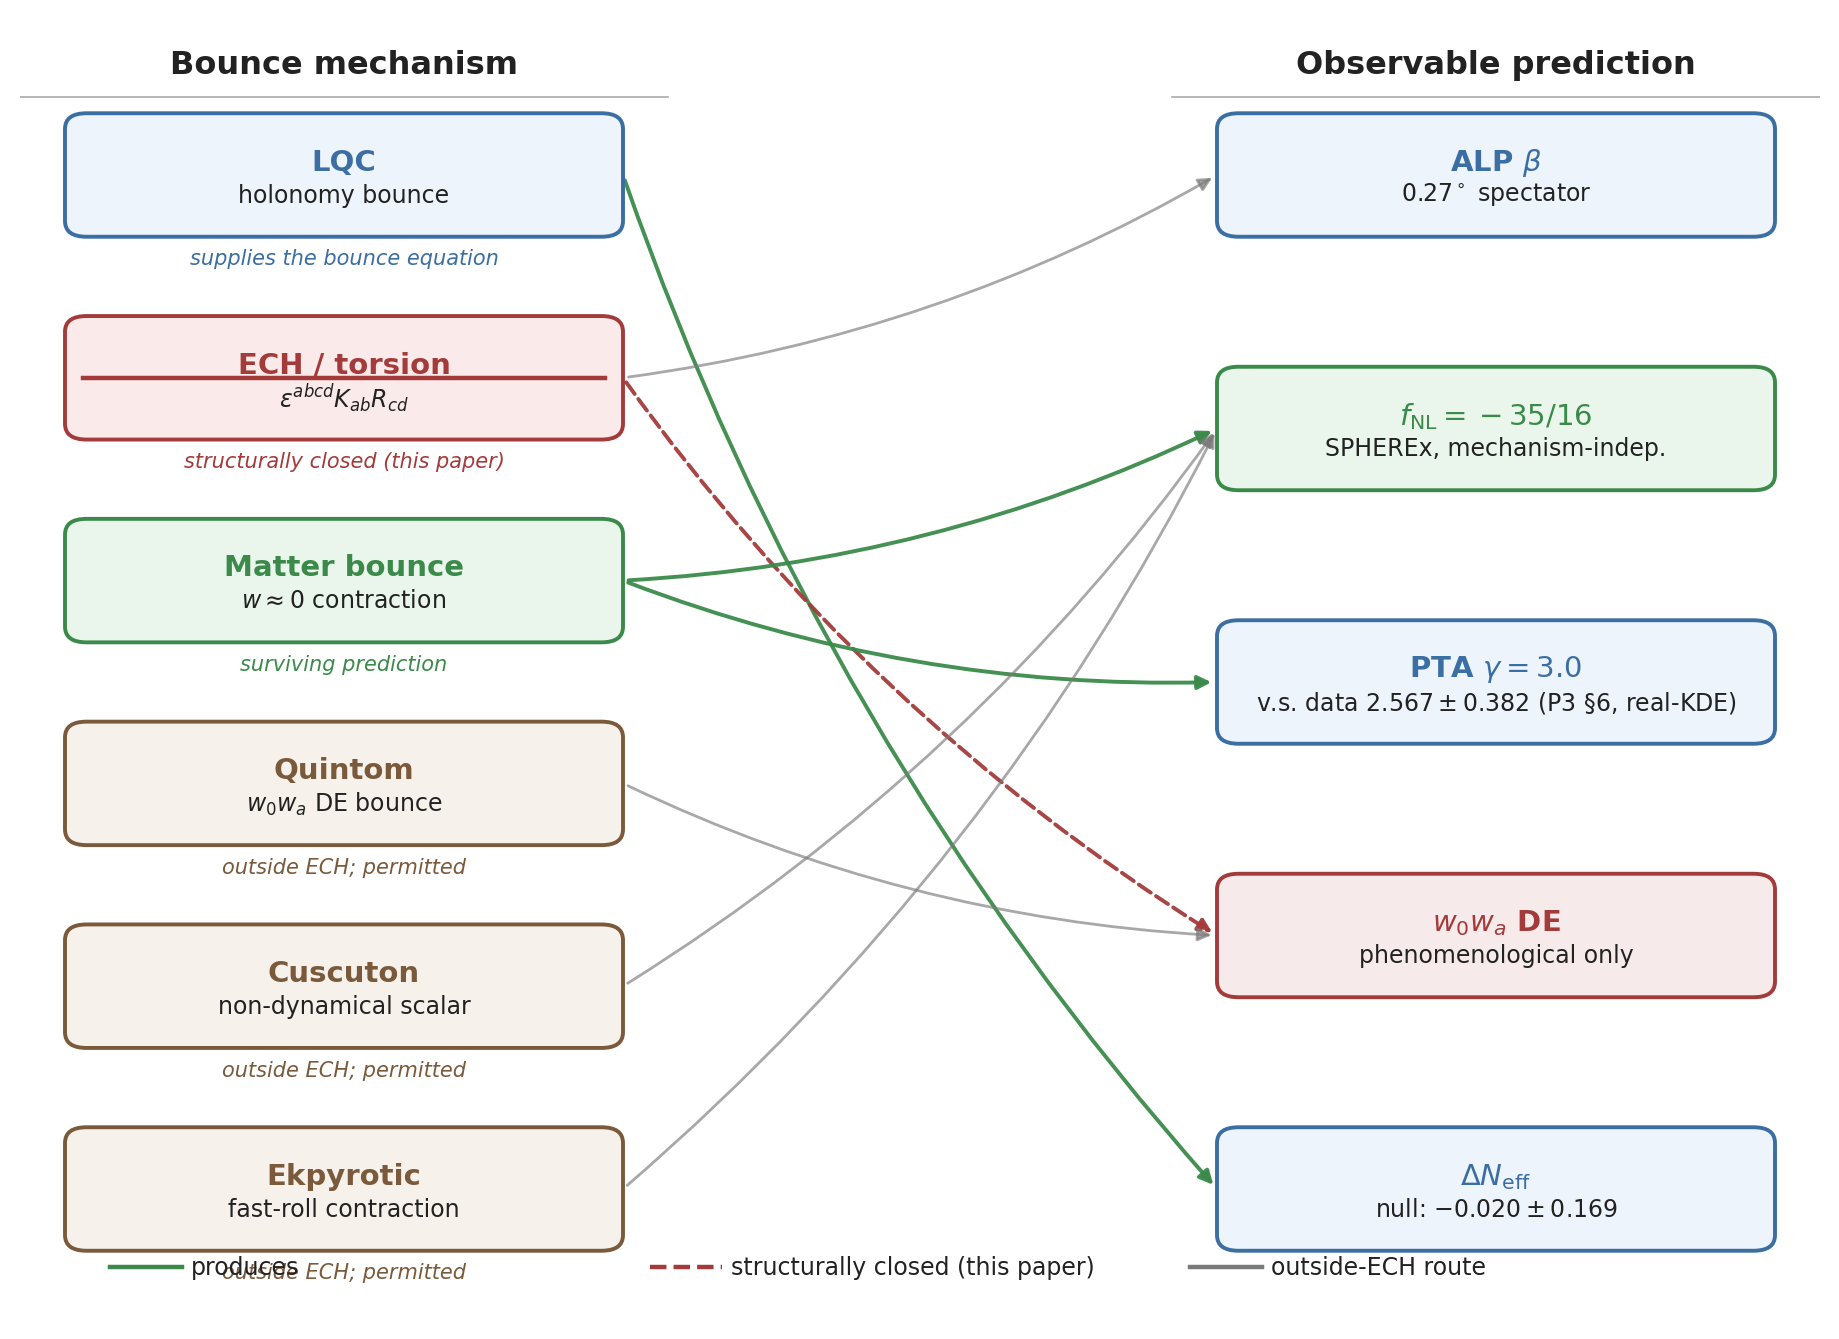
\includegraphics[width=0.95\textwidth]{fig_theory_map.png}
\caption{\label{fig:theory_map}
  Bounce-mechanism $\rightarrow$ observable-prediction map. Left column:
  candidate non-singular bounce mechanisms (LQC, ECH/torsion, matter
  bounce, quintom-B, Cuscuton, ekpyrotic). Right column: distinctive
  observable channels (ALP birefringence $\beta$, $f_{\rm NL} = -35/8$,
  PTA spectral index $\gamma$, $w_0$--$w_a$ DESI signatures, $\Delta\Neff$).
  Arrows indicate which mechanism produces each prediction. ECH appears
  bordered with a dashed box marked \emph{structurally closed (this
  paper)}---the 14-constraint catalog narrows minimal-ECH dark-energy
  routes to zero phenomenologically free pathways. The matter-bounce
  pathway appears bordered with a solid green box marked \emph{surviving},
  reflecting that the $f_{\rm NL} = -35/8$ prediction is mechanism-independent
  across all matter-bounce mechanisms (Cai \etal~\cite{Cai:2009fn},
  Wilson-Ewing~\cite{WilsonEwing2012}) and survives independently of any
  specific UV completion.}
\end{figure*}


\subsection{Theoretical Foundations and Novel Synthesis}\label{sec:foundations}

Our framework collects well-established theoretical components and tests them as a structural-closure no-go theorem on minimal ECH dark energy, with separately tractable phenomenological predictors (each consistent with, but not derived from, the ECH action):

\textit{Einstein-Cartan Theory.}---The inclusion of spacetime torsion coupled to fermionic spin has been extensively studied since the pioneering work of Hehl \etal~\cite{Hehl1976}. Pop\l{}awski~\cite{Poplawski2012,Poplawski2011} demonstrated that torsion-induced four-fermion interactions can generate a small positive cosmological constant through condensate formation, and that the parity-violating pseudoscalar density modifies this interaction, providing a candidate mechanism for dark energy generation. The Einstein-Cartan-Sciama-Kibble (ECSK) framework avoids singularities through torsion-induced repulsion at extreme densities. Recent work by Liu \etal~\cite{Liu2025} showed that Einstein-Cartan torsion is preferred over $\Lambda$CDM by AIC criteria, providing independent statistical support for torsion-based cosmology.

\textit{Loop Quantum Gravity and Parity Violation.}---The connection between LQG's Barbero-Immirzi parameter and parity-violating effects has been rigorously established by Freidel, Minic \& Takeuchi~\cite{Freidel2005} and Mercuri~\cite{Mercuri2006,Mercuri2009}. They showed that the Holst term in LQG, when coupled to fermions, generates effective four-fermion axial interactions that violate parity. The Barbero-Immirzi parameter $\gamma$, originally introduced as an ambiguity in the LQG quantization, acquires physical significance through its role in parity-violating observables.

\textit{Black Hole Universe Origin.}---Pop\l{}awski~\cite{Poplawski2016} pioneered the ``universe in a black hole'' scenario, demonstrating that every black hole with torsion spawns a non-singular, closed baby universe beyond its event horizon. His subsequent work~\cite{Poplawski2010} explored torsion as an alternative to cosmic inflation, with the baby universe inheriting angular momentum and developing a preferred cosmic axis, providing a candidate origin for observed cosmic anomalies.


\subsection{Original Contributions}\label{sec:contributions}

Each theoretical ingredient above has been studied independently. Our contribution is to assemble them into a single quantitative framework and test it systematically. The original contributions are:

%% TRIMMED: Condensed from 5 items to 3; removed DE scale motivation and inflationary suppression as standalone contributions (subsumed by items below)
\begin{enumerate}[leftmargin=*]
\item \textit{14-constraint catalog and perturbation-transparency observation}: Through 7 foundation studies and 17 research branches, we establish 14 independent structural constraints that map the minimal ECH parameter space and identify which dark-energy pathways survive without phenomenological assumption. The central result is that minimal ECH gravity is perturbation-transparent: for canonical scalar field matter, torsion vanishes at all perturbation orders, the Holst sector decouples cleanly from scalar/tensor observables, and tests of $\gamma$ shift to nonperturbative parity-violating channels (ALP birefringence, primordial gravitational waves).

\item \textit{Stock-CAMB $\Lambda$CDM$+\Delta\Neff$ proxy MCMC (null-consistency test, not an ECH module)}: Independent Cobaya runs across two frozen dataset combinations use stock CAMB with $\Delta\Neff$ as a free parameter; the Boltzmann code carries no spin-torsion modifications, so this is a null-consistency test of an extra radiation-like degree of freedom rather than evidence for the ECH theory. The runs find $\Delta\Neff$ consistent with zero and $H_0 = 67.68 \pm 1.06$, recovering standard Planck $\Lambda$CDM. The $\ln B = +4.8$ (full-tension dataset) reported in Sec.~\ref{sec:cosmo_fits} is dataset-dependent, computed via Savage-Dickey on a posterior with $r=-0.89$ correlation (which biases the estimator), and refers to $\Lambda$CDM$+\Delta\Neff$, \emph{not} to the spin-torsion theory; we treat it as indicative only.

\item \textit{ALP birefringence consistency check (secondary)}: A spectator ALP with natural parameters ($f_a \sim \MPl$, $m \sim H_0$) is consistent with the published Eskilt~\etal\ joint Planck+ACT value $\beta = 0.342^\circ \pm 0.094^\circ$ ($3.6\sigma$) without fine-tuning (R42 Wave 14-Y peer-review reframe, P1-OA-M3: the headline observational constraint is the published joint single-analysis $3.6\sigma$, not the simplified $3.9\sigma$ inverse-variance combination retained as an auxiliary cross-check in Sec.~\ref{sec:birefringence_check}, which neglects shared calibration systematics between Planck and ACT and inflates the apparent significance). This ALP model is a spectator field mechanism independent of the gravitational theory: the same $\beta \approx 0.27^\circ$ arises in standard GR with an identical ALP, so the result is \emph{not} a distinctive ECH prediction. We do not claim that ECH \emph{predicts} this value; we report only that it is consistent with the observed signal. The model class was previously studied by Fujita \etal~\cite{Fujita2021}; our contribution is the ECH-motivated parameter identification and independent MCMC inference, not the model itself. The result is a consistency check of the parity-violation signal, not a prediction of minimal ECH (which does not derive the photon-torsion coupling; see Sec.~\ref{sec:birefringence_check}).
\end{enumerate}

\subsection{Paper Organization}

This paper is organized as follows. Section~\ref{sec:theory} develops the theoretical framework. Section~\ref{sec:obs} presents observational signatures and evidence, including the independent MCMC verification (Sec.~\ref{sec:verification}). Sections~\ref{sec:derivations}--\ref{sec:data_cmb} summarize derivations and data methods (Supplementary material including MCMC chains, configuration files, and analysis scripts is available in the public repository at \url{https://github.com/Hubify-Projects/bigbounce} and will be deposited as an arXiv companion upon submission). Section~\ref{sec:cosmo_fits} presents cosmological fits and model comparison. Sections~\ref{sec:systematics}--\ref{sec:related} provide condensed systematic analysis, falsification criteria, and related work. The core results occupy Secs.~\ref{sec:barriers}--\ref{sec:loophole}: the 14 structural barriers, perturbation-transparency observation, and hybrid loophole rejection. Section~\ref{sec:discussion} discusses the inflationary suppression factor and birefringence analysis. Sections~\ref{sec:limitations}--\ref{sec:conclusions} address limitations and conclusions. Appendices provide the parameter summary (Appendix~\ref{app:params}), dimensional analysis (Appendix~\ref{app:dimensions}), reproducibility materials (Appendix~\ref{app:reproducibility}), and claims classification (Appendix~\ref{app:claims}).


%% ============================================================
%%  2. THEORETICAL FRAMEWORK
%% ============================================================
\section{Theoretical Framework}\label{sec:theory}

\subsection{Loop Quantum Cosmology and the Holst Action}\label{sec:holst}

\subsubsection{Einstein-Cartan-Holst Action}

The fundamental action combining Einstein-Cartan theory with the Holst term is
\begin{align}\label{eq:ECH}
S_{\rm ECH} &= \frac{1}{16\pi G} \int d^4x\, e \left[e^\mu_a\,e^\nu_b\,R^{ab}_{\;\;\;\mu\nu} + \frac{1}{\gamma} \varepsilon^{abcd}\,e_{a}^{\;\mu}\,e_{b}^{\;\nu}\,R_{cd\mu\nu} \right.\nonumber\\
&\qquad\left.+ \frac{1}{4} T^{abc} T_{abc}\right] + S_{\rm matter},
\end{align}
where $e = \det(e^a_\mu)$ is the tetrad determinant, $R^{ab}_{\;\;\;\mu\nu}$ is the curvature of the Lorentz connection, $\gamma$ is the Barbero-Immirzi parameter, and $T^{abc}$ is the torsion tensor. The Holst term $\varepsilon^{abcd}e_a^\mu e_b^\nu R_{cd\mu\nu}/\gamma$ is topological in the absence of torsion but contributes non-trivially when fermions are present. This construction builds directly on the foundational work of Freidel, Minic \& Takeuchi~\cite{Freidel2005}, who established that the Barbero-Immirzi parameter becomes physically observable through its coupling to fermionic matter. For historical clarity: Hehl~\etal~(1976)~\cite{Hehl1976} established the Einstein-Cartan framework for torsion coupled to fermion spin; the Holst term $\varepsilon^{IJKL}e_I\wedge e_J\wedge R_{KL}$ was introduced later by Holst~(1996)~\cite{Holst1996}.

Equation~\eqref{eq:ECH} presents the \textit{second-order} (metric) form of the ECH action, obtained after algebraic elimination of the torsion tensor via its own equation of motion (Eq.~\ref{eq:torsion} below). In this form, the $\frac{1}{4}T^{abc}T_{abc}$ term is a shorthand for the four-fermion contact interaction that results from integrating out the non-propagating torsion (see, e.g., Ref.~\cite{Hehl1976}). The coefficient $\frac{1}{4}$ is fixed by the Einstein-Cartan algebraic constraint $T^{a}_{\phantom{a}bc} = \kappa\,\epsilon^{a}_{\phantom{a}bcd}\,\bar{\psi}\gamma^{d}\gamma^{5}\psi$; it is not a free parameter. We do not vary the action with respect to torsion as an independent field---the variation is performed with respect to the metric $g_{\mu\nu}$ and the matter fields only. In the first-order (Palatini) formulation, torsion is determined algebraically by the spin density, and this term is not independently specified. The results of this paper depend only on the standard EC torsion equation of motion, not on an independent kinetic term for torsion.

\textit{Clarification on the first/second-order formalism.}---The presence of $T^{abc}$ in Eq.~\eqref{eq:ECH} might suggest a first-order (Palatini) treatment in which the connection is an independent variable. We emphasize that we work entirely in the second-order (metric) formalism throughout: the full connection is the Levi-Civita connection plus contorsion, $\Gamma^\lambda{}_{\mu\nu} = \mathring{\Gamma}^\lambda{}_{\mu\nu} + K^\lambda{}_{\mu\nu}$, where the contorsion $K^\lambda{}_{\mu\nu}$ is determined algebraically by the spin density of matter via the Cartan field equations (Eq.~\ref{eq:torsion}). For a canonical scalar field---the matter content relevant to all perturbation-level calculations in this paper---the spin density vanishes identically, torsion is zero, and the theory reduces exactly to general relativity with the Levi-Civita connection~\cite{Hehl1976}. The $T^{abc}T_{abc}$ term in Eq.~\eqref{eq:ECH} is therefore not an independently specified kinetic term; it is the residual contact interaction obtained \textit{after} solving the algebraic torsion equation and substituting back, as derived explicitly in Steps~1--2 below (Eqs.~\ref{eq:torsion}--\ref{eq:4fermi}). This is a standard and well-known feature of Einstein-Cartan theory; we state it explicitly to avoid any ambiguity about the variational principle employed.

The Barbero-Immirzi parameter is fixed by the LQG black hole entropy calculation~\cite{Ashtekar2011,ABCK1998}:
\begin{equation}\label{eq:gamma}
\gamma = 0.274 \pm 0.020,
\end{equation}
Different entropy-counting schemes yield different values: the Ashtekar-Baez-Corichi-Krasnov (ABCK) calculation~\cite{ABCK1998} gives $\gamma_{\rm ABCK} \approx 0.274$, while the Domagala-Lewandowski-Meissner (DLM) full SU(2) state counting~\cite{Domagala2004,Meissner2004} gives $\gamma_{\rm DLM} \approx 0.2375$. We adopt $\gamma = 0.274$ (ABCK) throughout this paper; the DLM value would shift $\rho_{\rm crit}$ upward to $\simeq 0.41\,\rho_{\rm Pl}$ without qualitatively changing any conclusion. Whether $\gamma$ constitutes a genuine physical observable or a quantization artifact absorbable by canonical transformations remains debated~\cite{Freidel2005,Mercuri2006}. This distinction does not affect our results at leading order: if $\gamma$ is non-physical, the torsion-fermion coupling factor $\gamma^2/(\gamma^2+1)$ in Eq.~\eqref{eq:4fermi} reverts to unity (the standard ECSK value), modifying the parity-odd coefficient by $\mathcal{O}(10\%)$ without eliminating parity violation, which originates from the Holst term's coupling to fermions independently of the Barbero-Immirzi interpretation.

\begin{figure}[t]
\centering
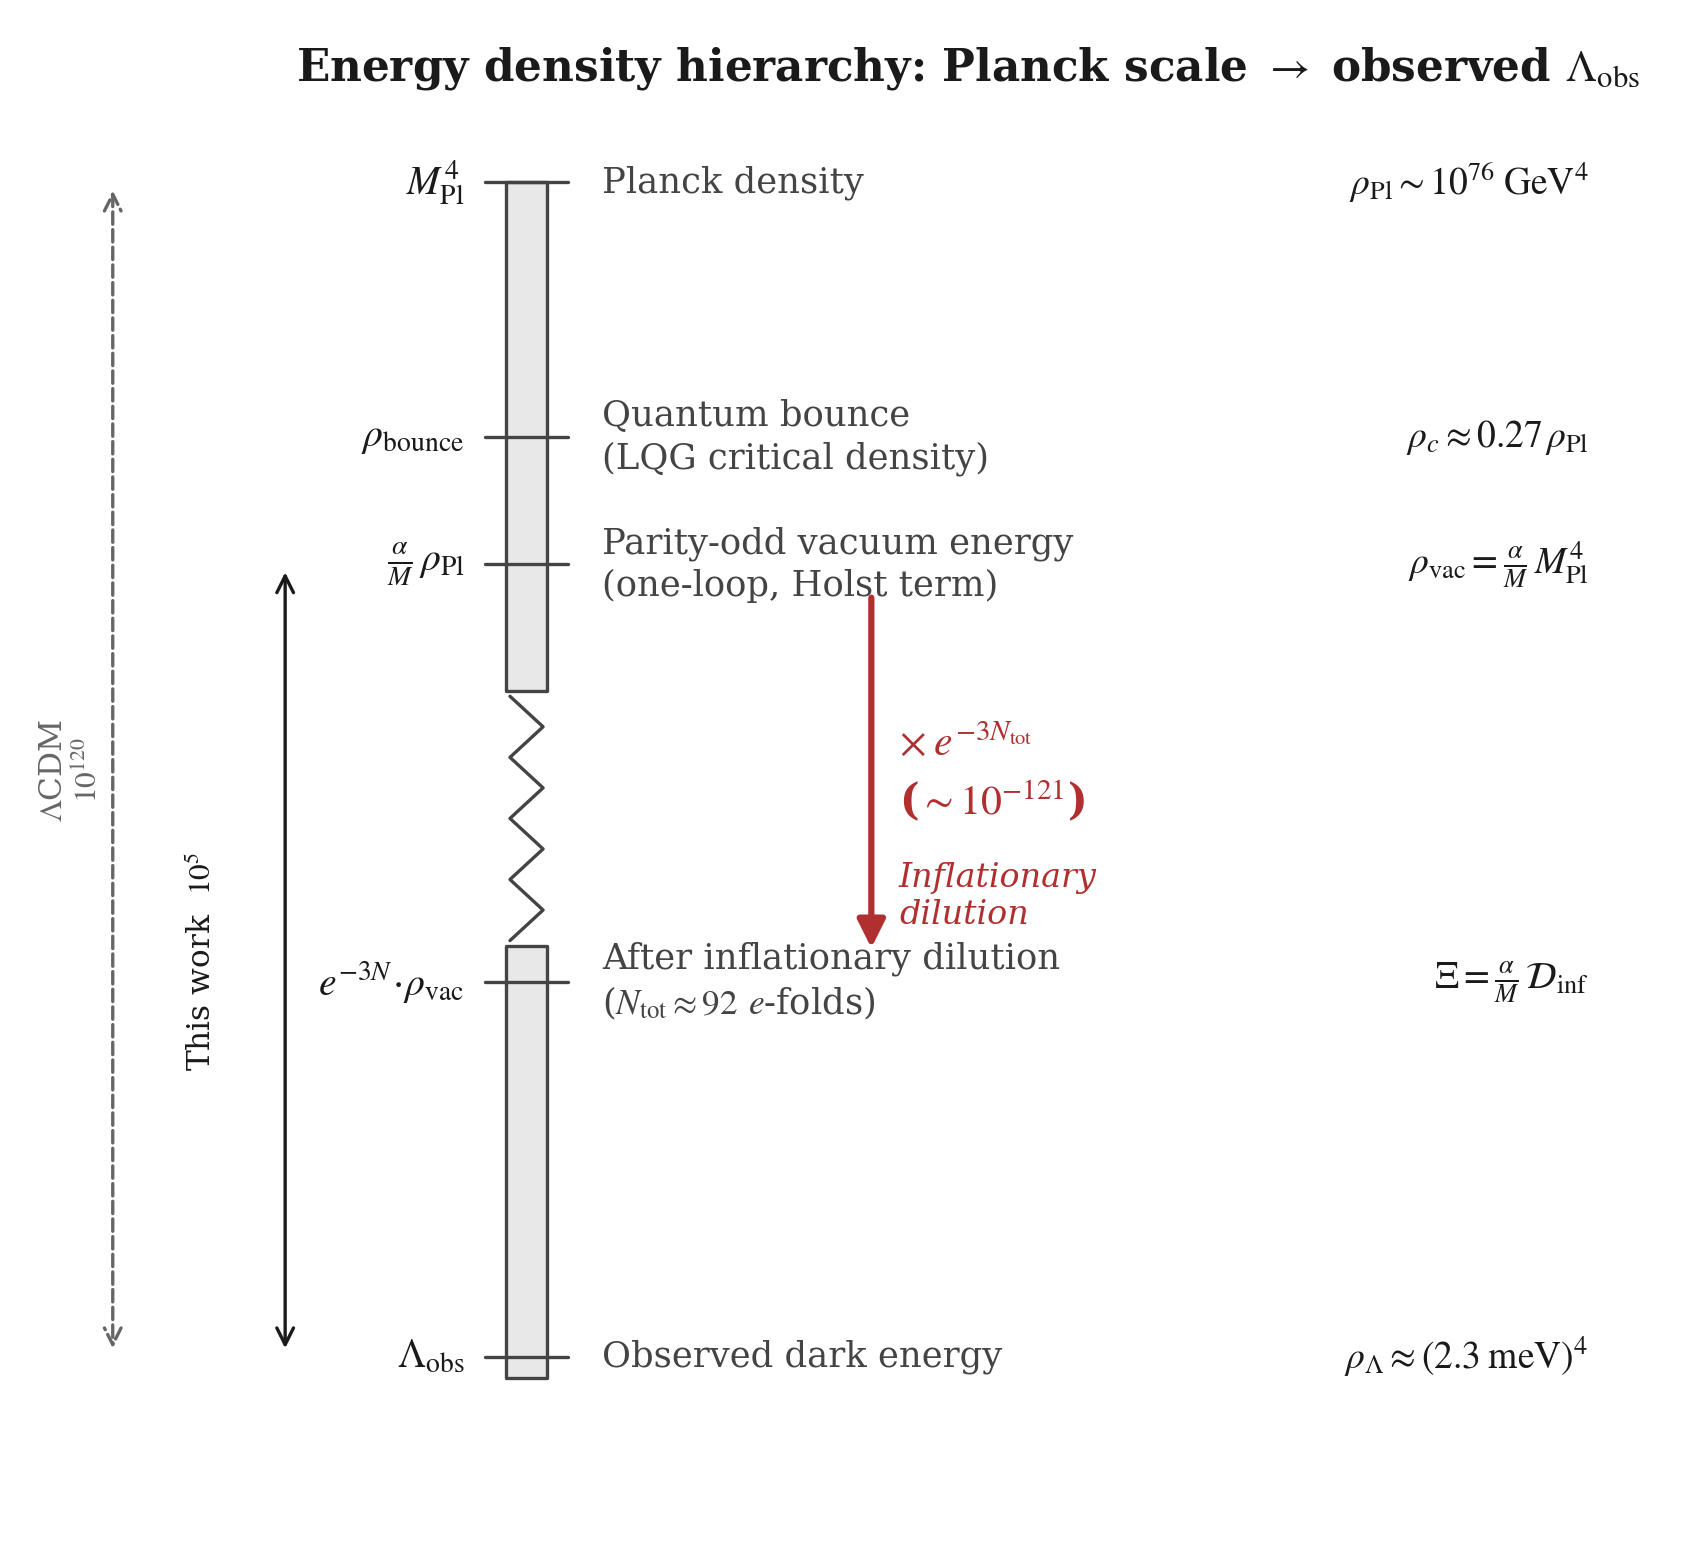
\includegraphics[width=0.98\columnwidth]{figures/figure1_lqg_holst_derivation_enhanced.png}
\caption{\label{fig:derivation} Energy density hierarchy from the Planck scale to the observed dark energy scale, illustrating the phenomenological scaling ansatz $\rho_{\rm vac}\sim[(\alpha/M)\,\MPl]\,M_{\rm Pl}^4$ (Sec.~\ref{sec:parityodd}, Appendix~\ref{app:dimensions}). This ansatz is dimensionally correct on-shell at the bounce but is \emph{not} derived from the ECH action; the connection from the Holst sector to the late-time $\rho_\Lambda$ requires phenomenological assumption beyond the minimal framework (see body text for the explicit statement). Inflationary dilution by $\sim e^{-3N_{\rm tot}}$ bridges the gap to the observed $\rho_\Lambda\approx (2.3\;\text{meV})^4$. Left axis: comparison of the residual fine-tuning in this framework ($10^5$, from uncertainty in $N_{\rm tot}$) versus $\Lambda$CDM ($10^{120}$).}
\end{figure}


\subsubsection{Derivation of the Parity-Odd Term}\label{sec:parityodd}

Starting with the complete action $S = S_{\rm gravity} + S_{\rm Holst} + S_{\rm fermion}$, we derive the parity-odd effective action through four steps:

\textit{Step~1: Torsion Activation.}---When fermions are minimally coupled to gravity with torsion, the torsion tensor is determined algebraically by the fermionic spin density:
\begin{equation}\label{eq:torsion}
T^{abc} = 8\pi G\, S^{abc},
\end{equation}
where $S^{abc} = \frac{1}{4}\bar{\psi}\gamma^{[a}\gamma^{bc]}\psi$ is the fermionic spin density tensor (we use natural units $c=\hbar=1$ throughout; full notation and conventions are summarized in the supplementary material accompanying the public repository, Appendix~\ref{app:reproducibility}). Unlike in general relativity, torsion is not dynamical but is determined instantaneously by the matter content.

\textit{Step~2: Four-Fermion Contact Interaction.}---Substituting Eq.~\eqref{eq:torsion} back into the action and integrating out torsion yields an effective four-fermion interaction~\cite{Hehl1976}:
\begin{equation}\label{eq:4fermi}
\mathcal{L}_{\rm int} = -\frac{3\pi G_N}{2}\times \frac{\gamma^2}{\gamma^2+1}\times J^5_{\mu}\,J^{5\mu},
\end{equation}
where $J^{5\mu}=\bar{\psi}\gamma^{\mu}\gamma^5\psi$ is the axial current. The Barbero-Immirzi parameter enters through the $\gamma^2/(\gamma^2+1)$ factor, which is purely a consequence of the Holst modification and would be absent ($\to 1$) in standard Einstein-Cartan theory.

\textit{Step~3: Parity-Odd Effective Action.}---The effective action acquires a parity-odd term through quantum corrections, as shown by Mercuri~\cite{Mercuri2009}. The origin of this term is the Holst term: in first-order variables (tetrad $e^I$ and Lorentz connection $\omega^{IJ}$, with $I,J,\dots$ internal Lorentz indices), the ECH action's parity-odd piece is
\begin{equation}\label{eq:Holst4form}
S_{\rm Holst} = \frac{\MPl^2}{\gamma}\int e_I\wedge e_J\wedge R^{IJ}(\omega),
\end{equation}
where $R^{IJ}=d\omega^{IJ}+\omega^{I}_{\;\;K}\wedge\omega^{KJ}$ is the curvature 2-form. This is a manifestly diffeomorphism-invariant 4-form (two tetrad 1-forms $\wedge$ one curvature 2-form). When the connection is decomposed as $\omega^{IJ}=\mathring{\omega}^{IJ}+K^{IJ}$ (Levi-Civita $+$ contorsion), Eq.~\eqref{eq:Holst4form} generates terms involving contorsion coupled to curvature. After integrating out torsion (which is algebraically determined by fermion spin density, Eq.~\ref{eq:torsion}) and including quantum corrections at one loop, the effective parity-odd action takes the form
\begin{equation}\label{eq:Seff}
S_{\rm eff} = \frac{\alpha}{M}\int e_I\wedge e_J\wedge \mathcal{F}^{IJ}[K,\mathring{R}],
\end{equation}
where $\mathcal{F}^{IJ}$ collects the contorsion-dependent pieces ($\mathring{D}K^{IJ}+K^{I}_{\;\;K}\wedge K^{KJ}$ at leading order), $M = M_{\rm area\text{-}gap}\sim\sqrt{\gamma}\,\MPl$ is the LQG area-gap mass scale, and $\alpha$ is a \textit{dimensionless} coupling ($[\alpha]=M^0$). In components, the leading contribution reduces to
\begin{equation}\label{eq:Seff_comp}
S_{\rm eff} = \int d^4x\,\sqrt{-g}\;\frac{\alpha}{M}\;\varepsilon^{\mu\nu\rho\sigma}\,e^I_\mu\,e^J_\nu\,\mathcal{F}_{IJ\rho\sigma},
\end{equation}
where the operator $\varepsilon^{\mu\nu\rho\sigma}e^I_\mu e^J_\nu\mathcal{F}_{IJ\rho\sigma}$ has mass dimension~$+2$ and $\alpha/M$ has dimension~$-1$, giving a total Lagrangian density of mass dimension~$+1$---three short of the required~$+4$ (see Appendix~\ref{app:dimensions} for the full counting).

We emphasize that the operator in Eq.~\eqref{eq:Seff_comp} has naive mass dimension $[\mathcal{L}_{\rm odd}] = +1$ in the Lagrangian density, three units short of the required $+4$. The evaluation at Planck-scale densities ($K \sim \MPl$, $R \sim \MPl^2$) that yields $\rho_\Lambda = \Xi\,\MPl^4$ is therefore a \textit{scaling ansatz}, not a controlled effective field theory calculation. A rigorous EFT treatment would require either (a)~identifying the correctly dimensioned operator from the full set of dimension-4 parity-odd invariants, or (b)~demonstrating that the on-shell evaluation is protected by a symmetry (e.g., a non-renormalization theorem in the torsionful sector). We proceed with the scaling ansatz as a phenomenological parameterization, noting that the 14 structural barriers identified in Secs.~\ref{sec:barriers}--\ref{sec:loophole} close the bounce-to-dark-energy route independently of whether this dimensional gap can be resolved. Throughout this paper, we adopt the convention that the Einstein-Hilbert action carries the standard $\MPl^2/2$ prefactor, while the parity-odd sector carries $\alpha/M$ independently.

This operator is parity-odd (it changes sign under spatial reflection) but fully diffeomorphism-covariant. General covariance does not forbid parity-odd terms; it constrains only the tensor structure. Since classical gravity preserves parity, the coefficient $\alpha/M$ must be generated through quantum corrections.

\textit{Notation.}---For brevity, we sometimes write the component-form integrand as ``$\varepsilon^{abcd}K_{ab}R_{cd}$'' (where $a,b,c,d$ are internal Lorentz indices) as shorthand for the full 4-form expression Eq.~\eqref{eq:Seff}. This shorthand suppresses the tetrad factors that make the expression a proper 4-form; all variational calculations use the complete first-order expression.

\textit{Torsion remains algebraic.}---The effective action $S_{\rm eff}$ (Eq.~\ref{eq:Seff}) contains derivatives of the contorsion through $\mathring{D}K^{IJ}$ in $\mathcal{F}^{IJ}$, which could in principle promote torsion from algebraic to dynamical. The kinetic correction to the algebraic Einstein--Cartan torsion equation enters at relative size $\mathcal{O}\!\left((\alpha/M)\,k\right)$, where $k$ is the relevant gradient scale of the contorsion (the algebraic source $\sim\MPl^2 K$ comes from the standard Einstein--Cartan piece, while the kinetic piece scales as $(\alpha/M)\,k\,\MPl^2 K$, so the dimensionless ratio is $(\alpha/M)\,k$, not $(\alpha/M)\,\MPl^2$ which would carry units of mass). With $\alpha/M\sim 10^{-21}\;\text{GeV}^{-1}$, this ratio is $\sim 10^{-2}$ at the Planck-scale bounce ($k\sim\MPl$, recovering the $[(\alpha/M)\MPl]\sim 10^{-2}$ value already cited in the next subsection), $\sim 10^{-5}$ at the GUT/reheating scale ($k\sim M_{\rm GUT}\sim 10^{16}\,\text{GeV}$), and exponentially smaller at all later cosmological scales. \textbf{R42 Wave 14-M peer-review reframe (cross-model OpenAI P1-OA-B4):} an earlier draft wrote this correction as $\mathcal{O}(\alpha/M\,\MPl^2)\sim 10^{-3}$, but $(\alpha/M)\,\MPl^2$ has mass dimension $+1$, not $0$, so the unitless ``$10^{-3}$'' figure was dimensionally ill-posed. The scale-aware estimate above replaces it. Torsion therefore remains effectively algebraic (determined instantaneously by the spin density) at all gradient scales $k\ll \MPl/(\alpha/M\,\MPl)\sim\MPl/10^{-2}$, which covers every sub-Planckian cosmological epoch. A full stability analysis (ghost/tachyon checks) of the modified torsion sector is warranted but is not expected to reveal pathologies at this suppression level.

\textit{Step~4: Parity-Odd Coefficient.}---The existence of a finite parity-odd coefficient is motivated by one-loop estimates in a torsionful background. Following the one-loop analyses of Freidel \etal~\cite{Freidel2005} and Shapiro \& Teixeira~\cite{ShapiroTeixeira2014}, which established the divergence structure and renormalization of the effective Barbero-Immirzi parameter, the expected order of magnitude is
\begin{equation}\label{eq:oneloop}
\frac{\alpha}{M}\sim \frac{g^2}{32\pi^2}\,\frac{\gamma}{M}\,\ln\!\left(\frac{\Lambda_{\rm UV}^2}{\mu^2}\right)+\delta_{\rm NY},
\end{equation}
where $g$ is the effective dimensionless axial--torsion Yukawa coupling defined by the vertex $g\,\bar{\psi}\gamma^5\gamma^a\psi\,K_a$ (with $g^2\sim 8\pi G_N M^2\,\gamma^2/(\gamma^2+1)\sim\mathcal{O}(1)$ at the area-gap scale), $\Lambda_{\rm UV}$ is a UV scale, $\mu$ is the renormalization scale, and $\delta_{\rm NY}$ encodes the finite Nieh--Yan contribution whose precise value depends on the regularization scheme---particularly the treatment of $\gamma_5$ in dimensional regularization~\cite{ShapiroTeixeira2014} (the 't~Hooft--Veltman and Breitenlohner--Maison prescriptions yield different finite parts for parity-odd traces). We therefore \textbf{treat $\alpha/M$ as a phenomenological parameter constrained by data} (see Table~\ref{tab:priors}), with Eq.~\eqref{eq:oneloop} providing the theoretical motivation for its existence and order of magnitude ($[(\alpha/M)\,\MPl]\sim 10^{-2}$), not a controlled first-principles prediction.

A one-loop RG estimate suggests logarithmic running:
\begin{equation}\label{eq:RGflow}
\frac{d\alpha}{d\ln\mu} \sim -\frac{g^2}{16\pi^2}\times 2N_f,
\end{equation}
where $N_f$ is the number of fermion species contributing at scale~$\mu$. This one-loop result is scheme-dependent and included to illustrate the qualitative running behavior; it has no scheme-independent predictive content at this order. However, this equation inherits the same scheme dependence as the coefficient itself: its derivation requires specifying how $\gamma_5$ is handled in $d=4-\epsilon$ dimensions and which counterterm conventions are adopted for the Nieh--Yan sector. The physical content is that $\alpha$ runs weakly (the loop factor $g^2/(16\pi^2)\sim 10^{-3}$ ensures perturbative suppression), so its value is approximately scale-independent over cosmological history. A controlled derivation of $\alpha/M$ from non-perturbative quantum gravity (spin-foam amplitudes or lattice methods) remains an important open problem (Sec.~\ref{sec:futuredirections}).


%% TRIMMED: Parameter Naturalness subsection condensed to 2 sentences
\subsubsection{Parameter Naturalness}\label{sec:naturalness}
The parent black hole mass must exceed $M_{\rm crit} = (M_{\rm Pl}^4/\rho_{\rm vac})^{1/3}\approx 10^{-3}M_\odot$, easily satisfied by any astrophysical black hole. The required dilution of inherited rotation is naturally achieved through $\sim 50$ $e$-folds of inflation.


\subsection{Black Hole Interior and Quantum Bounce}\label{sec:bounce}

In Loop Quantum Cosmology (LQC), holonomy corrections to the gravitational Hamiltonian constraint produce a non-singular bounce at Planck-scale densities~\cite{Ashtekar2011}. The effective Friedmann equation is\footnote{The LQC bounce (from quantum geometry holonomy corrections) is physically distinct from the Einstein-Cartan torsion bounce of Pop\l{}awski~\cite{Poplawski2012}, which produces a qualitatively similar $\rho^2$ repulsion through classical spin-torsion coupling at high fermion density. In this paper, we adopt the LQC effective equation for its well-studied perturbation dynamics. The ECH framework provides the broader theoretical context for the parity structure (Sec.~\ref{sec:parityodd}) but is not the source of Eq.~\eqref{eq:modfriedmann}.}
\begin{equation}\label{eq:modfriedmann}
H^2 = \frac{8\pi G}{3}\,\rho\left[1-\frac{\rho}{\rhocrit}\right],
\end{equation}
where the critical density is
\begin{equation}\label{eq:rhocrit}
\rhocrit = \frac{3}{8\pi G\,\gamma^2\,\Delta} = \frac{\sqrt{3}}{32\pi^2\gamma^3}\,\rhoPl \simeq 0.27\,\rhoPl,
\end{equation}
with $\Delta = 4\sqrt{3}\pi\gamma\,\ell_P^2$ being the LQG area gap and $\rhoPl\equiv c^5/(\hbar G^2)$. The numerical value $\rhocrit \simeq 0.27\,\rhoPl$ corresponds to $\gamma = 0.274$ (ABCK); the DLM value $\gamma = 0.2375$ gives $\rhocrit \simeq 0.41\,\rhoPl$~\cite{Ashtekar2011}. The range $\gamma \in [0.2375, 0.294]$ brackets both counting schemes and gives $\rhocrit \in [0.22, 0.41]\,\rhoPl$. The factor $(1-\rho/\rhocrit)$ ensures that $H^2 \to 0$ as $\rho \to \rhocrit$, producing a smooth bounce. Key properties of the bounce:

\begin{itemize}[leftmargin=*]
\item For $\rho \ll \rhocrit$: standard GR is recovered exactly.
\item For $\rho \to \rhocrit$: $H \to 0$ (the universe momentarily stops expanding/contracting).
\item For $\rho$ slightly below $\rhocrit$ (contracting phase): $\dot{H} > 0$, triggering the bounce.
\item The bounce creates a new expanding region with initial conditions completely determined by the parent black hole properties, with no free parameters.
\end{itemize}

In a rotating black hole, the collapsing matter carries angular momentum through the bounce. The baby universe inherits this rotation, establishing a preferred cosmic axis $\hat{\omega}^a$. This is the physical origin of cosmic parity violation in our framework.


%% TRIMMED: Cosmic Rotation and Dark Energy subsection heavily condensed — detailed vorticity/Raychaudhuri/galaxy spin mechanism moved to supplementary material
\subsection{Cosmic Rotation and Dark Energy}\label{sec:rotation}

The effective cosmological constant in our framework is parameterized as:
\begin{align}\label{eq:Leff_full}
\boxed{\Leff = \Xi\,\MPl^2 + c_\omega\omega^2,}\quad
\Xi\equiv \left[\frac{\alpha}{M}\,\MPl\right]\Dinf,
\end{align}
\label{eq:Leff}%
where the first term identifies the parity-odd vacuum energy with the cosmological constant (a central \textit{assumption}, not a derivation) and $c_\omega\omega^2$ is the vorticity contribution from the $1+3$ covariant decomposition~\cite{Ellis1989}. CMB isotropy bounds give $(\omega/H)_0 < 5\times 10^{-11}$~\cite{Saadeh2016}, so $|c_\omega|\omega^2/H_0^2 < 2.5\times 10^{-21}$---rotation is completely negligible for background expansion. The dark energy scale is set entirely by $\Xi \sim 10^{-123}$ (Sec.~\ref{sec:gdp}).

We emphasize that Eq.~\eqref{eq:Leff_full} is a \textit{phenomenological parameterization}, not a first-principles derivation from the ECH action. The underlying parity-odd operator (Eq.~\ref{eq:Seff_comp}) has naive mass dimension $+1$ in the Lagrangian density, three short of the required $+4$. Explicitly,
\begin{equation}\label{eq:dimcount}
[\alpha/M] = -1, \quad [\varepsilon^{\mu\nu\rho\sigma}e^I_\mu e^J_\nu \mathcal{F}_{IJ\rho\sigma}] = +2 \;\Longrightarrow\; [\mathcal{L}_{\rm odd}] = +1,
\end{equation}
so the Lagrangian density is off-shell short by three powers of mass relative to the canonical $+4$ requirement (full on-shell evaluation chain in Appendix~\ref{app:dimensions}); the identification $\rho_\Lambda = \Xi\,\MPl^4$ relies on evaluating the operator on shell at Planck-scale bounce densities ($K \sim \MPl$, $R\sim\MPl^2$), which supplies the missing mass dimensions as a \textit{scaling ansatz} rather than a controlled EFT derivation. Correspondingly, the coefficient $c_\omega$ must carry dimensions of $[\text{length}]^{-2}$ (equivalently $[\text{mass}]^{+2}$) to produce a cosmological constant with the correct dimensions of $[\text{mass}]^{+2}$ from $\omega^2$ (which is dimensionless in natural units as a ratio $\omega/H$). No first-principles derivation of $c_\omega$ from the ECH action exists; the scaling $c_\omega \propto H_0^2$ is an ansatz motivated by dimensional analysis. The 14 structural barriers cataloged in Sec.~\ref{sec:barriers} close all known routes from deriving this parameterization from the fundamental ECH dynamics, establishing that the bounce-to-dark-energy connection is phenomenological at every level. The ``fine-tuning reduction from $10^{120}$ to $10^5$'' reparameterizes the hierarchy as sensitivity to $N_{\rm tot}$ (Sec.~\ref{sec:gdp}) but does not constitute a solution to the cosmological constant problem.

\subsubsection{Inflationary Suppression}\label{sec:dilution}

The contorsion $K_{ab}$, sourced by the fermion spin density, dilutes as $a^{-3}$ during inflation. The dilution factor is:
\begin{equation}\label{eq:Dinf}
\Dinf = \exp[-3N_{\rm tot}] \times \left(\frac{T_{\rm reh}}{M_{\rm GUT}}\right)^{3/2}.
\end{equation}
Matching $\rho_\Lambda \approx (2.3\;\text{meV})^4$ requires $N_{\rm tot} \approx 92$ (a fitted parameter, not predicted), reducing fine-tuning from $10^{120}$ to $\sim 10^5$ as sensitivity to $\Delta N_{\rm tot} \approx 4$ $e$-folds. This reparameterizes the fine-tuning problem as an initial-condition question (``why $\sim$92 $e$-folds?'') rather than a fundamental-constant question, but does not solve the cosmological constant problem.

We \textit{assume} $w = -1$ at late times; deriving this requires showing that the early-universe spin-torsion operator generates an IR-constant vacuum term, which has not been achieved. Four minimal routes (NJL condensate, one-loop effective action, dynamical Immirzi field, parity-sensitive CMB phenomenology) all yield negative results~\cite{Golden2026supplement}.

\subsubsection{Galaxy Spin Alignment Mechanism}\label{sec:spinmech}

The galaxy spin asymmetry amplitude evolves as
\begin{equation}
A(z) = A_0(1+z)^{-p}e^{-qz}, \qquad A_0 \in [0,0.02],
\label{eq:Az}
\end{equation}
with $A_0$ the present-day amplitude. The parity-odd operator introduces systematic chirality into the tidal field, but the framework's coupling $\alpha/M \sim 10^{-21}\;\text{GeV}^{-1}$ underpredicts any plausible spin asymmetry by $>100$ orders of magnitude. An independent ViT-Small classifier (93.7\% three-class validation accuracy, eight bias-hardening tests passed) applied to $8{,}474{,}531$ galaxies from DESI Legacy Imaging Surveys DR8 confirms the null: $\fcw^{\rm eq} = 0.5012 \pm 0.0006$\footnote{\label{fn:fcw}The value $\fcw^{\rm eq} = 0.5012 \pm 0.0006$ is measured on the benchmark-overlap subset where Galaxy Zoo labels are available for validation; the full-catalog equivariant value is $\fcw^{\rm eq} = 0.4974 \pm 0.0003$. Both are consistent with parity conservation; the monopole offset of $2.0\sigma$ in the benchmark subset is attributed to sub-percent classifier systematic.} (all-sky dipole at $0.43\sigma$). Galaxy spin asymmetry is not a prediction of the theory, and no significant signal exists to explain.


%% ============================================================
%%  3. OBSERVATIONAL PREDICTIONS AND EVIDENCE
%% ============================================================
\section{Observational Signatures and Evidence}\label{sec:obs}

\subsection{CMB $E$-$B$ Cross-Correlations}\label{sec:EB}

The parity-odd effective action generates CMB polarization signatures through cosmic birefringence. The parity-odd operator rotates the CMB polarization plane by a small angle~$\beta$. For a spatially uniform (isotropic) rotation, the standard result~\cite{Minami2020} is
\begin{equation}\label{eq:ClEB}
C_\ell^{EB}\approx \frac{\sin 4\beta}{2}\left(C_\ell^{EE}-C_\ell^{BB}\right) \approx 2\beta\left(C_\ell^{EE}-C_\ell^{BB}\right),
\end{equation}
where the small-angle approximation holds for $\beta\ll 1$~rad. This produces nonzero $EB$ power \textit{across all multipoles}, tracking the $EE-BB$ spectrum shape---not localized to any particular $\ell$ range. Similarly, the induced $TB$ cross-correlation is $C_\ell^{TB}\approx 2\beta\,C_\ell^{TE}$.

\textit{Connecting to Planck.}---The Planck measurement reports $\beta \approx 0.30^\circ$ at $2.4$--$2.7\sigma$~\cite{Minami2020,Eskilt2022}. Our framework's parity-odd operator (Eq.~\ref{eq:Seff}) is qualitatively consistent with cosmic birefringence, since it violates parity. However, deriving the photon polarization rotation angle $\beta$ from our gravitational/torsion operator requires an explicit effective coupling between the parity-odd sector and the electromagnetic field---for example, a term of the standard axion-like form
\begin{equation}\label{eq:axionFF}
\mathcal{L}\supset \frac{\varphi(\tau)}{4f}\,F_{\mu\nu}\tilde{F}^{\mu\nu},
\end{equation}
where $\varphi$ is a pseudo-scalar field sourced by the spin-torsion sector and $f$ is the associated decay constant, generated by integrating out torsion at one loop with an electromagnetic vertex. This coupling has not yet been derived in this work. We therefore treat the consistency between our framework's parity violation and the observed $\beta\approx 0.30^\circ$ as suggestive, not as a quantitative prediction.

\textit{Relation between $\varphi/f$ and $\beta$.}---For a spatially uniform pseudo-scalar rolling over conformal time, the standard result~\cite{CarrollFieldJackiw1990,Carroll1998} gives a uniform polarization rotation $\beta = \Delta\varphi/(2f)$, where $\Delta\varphi$ is the net field excursion between last scattering and today. This relation assumes three conditions: (i)~spatial uniformity of $\varphi$ over the last-scattering surface (justified if the correlation length exceeds the Hubble radius at decoupling), (ii)~photon propagation along FLRW geodesics (valid for the isotropic component), and (iii)~$\varphi/f\ll 1$ so that the rotation is in the small-angle regime (consistent with $\beta\approx 0.30^\circ \approx 5\times 10^{-3}$~rad). Deriving $\varphi$ and $f$ from the spin-torsion operator $(\alpha/M)\varepsilon^{abcd}K_{ab}R_{cd}$ requires computing the one-loop photon-torsion vertex and matching to the effective Lagrangian~\eqref{eq:axionFF}; this calculation is beyond the scope of the present work. We use the literature values of $\beta$ as consistency benchmarks throughout.

\textit{Anisotropic component.}---In addition to the uniform rotation, the cosmic rotation axis defines a preferred direction $\hat{n}$, which introduces an \textit{anisotropic} birefringence field $\beta(\hat{n})$ with power concentrated at low multipoles. This anisotropic component contributes primarily to off-diagonal $\ell$-$\ell'$ correlations (detectable via quadratic estimators~\cite{Eskilt2022}), with additional diagonal power at $\ell\lesssim 10$. For the spectator-ALP model (Sec.~\ref{sec:birefringence_check}), a spatially homogeneous ALP condensate at the bounce epoch predicts negligible anisotropic birefringence: $A_{\rm CB} \sim \beta^2 (\delta\varphi/\Delta\varphi)^2 \approx 7 \times 10^{-12}\;\text{deg}^2$, which is ${\sim}10^{10}$ times below the current Planck 95\% upper limit ($A_{\rm CB} < 0.033\;\text{deg}^2$~\cite{Namikawa2020}) and undetectable even by CMB-S4. This constitutes a \emph{falsifiable prediction}: detection of significant anisotropic birefringence would exclude the bounce-ALP interpretation. Alternative models predict different angular spectra:
\begin{itemize}[leftmargin=*]
\item \textit{Axion cosmic birefringence}: Scale-invariant power in $\beta(\hat{n})$, producing $EB$ correlations across all~$\ell$.
\item \textit{Chern-Simons gravity}: Peaks at $\ell\sim 100$--$1000$.
\item \textit{Spin-torsion (this work)}: Dominantly isotropic birefringence ($\beta \approx 0.27^\circ$) from a spatially homogeneous spectator ALP, with anisotropic power suppressed by $({\delta\varphi}/{\Delta\varphi})^2 \sim 10^{-10}$ ($A_{\rm CB} \sim 7 \times 10^{-12}\;\text{deg}^2$, undetectable by current and next-generation experiments).
\end{itemize}

Observational support comes from Minami \& Komatsu~\cite{Minami2020}, who found cosmic birefringence in Planck data at $\beta\approx 0.35^\circ\pm 0.14^\circ$, inconsistent with $\beta=0$ at $2.4\sigma$. Subsequent analysis by Eskilt~\cite{Eskilt2022} found $\beta = 0.30^\circ \pm 0.11^\circ$ ($2.7\sigma$). A dedicated ACT DR6 analysis by Diego-Palazuelos \& Komatsu~\cite{DiegoPalazuelos2025} measured $\beta = 0.215^\circ \pm 0.074^\circ$ ($2.9\sigma$), providing independent confirmation from a different instrument. Joint constraints combining birefringence with early dark energy and DESI+Planck data have been explored by Yin \etal~\cite{Yin2026}, demonstrating that nonzero $\beta$ is compatible with---and potentially complementary to---solutions to the $H_0$ tension. A combined analysis by the SPIDER collaboration~\cite{SPIDER2025} using SPIDER, Planck, and ACT data yields a total polarization rotation angle (instrumental $\alpha$ + cosmological $\beta$) detected at ${\sim}7\sigma$, though cleanly separating the instrumental and cosmological contributions remains an active challenge. The combined significance depends sensitively on the treatment of shared calibration systematics between Planck and ACT~\cite{ACT2024}.

\textit{Calibration caveat.}---The cosmic birefringence signal is degenerate with miscalibration of the instrumental polarization angle~$\psi$~\cite{Minami2020}. Minami \& Komatsu's method breaks this degeneracy using the galactic foreground $EB$ signal as a self-calibration anchor, assuming vanishing intrinsic foreground $EB$---an assumption that has been questioned for polarized thermal dust. Independent validation from experiments with different optics and calibration strategies (Simons Observatory, LiteBIRD) is essential. The isotropic birefringence value ($\beta\approx 0.30^\circ$) can be tested with existing and near-term data; the anisotropic low-$\ell$ component requires full-sky, cosmic-variance-limited polarimetry (LiteBIRD).

\textit{Detectability.}---The isotropic signal has been detected at $2.4$--$2.7\sigma$ by Planck and $2.9\sigma$ by ACT~DR6~\cite{DiegoPalazuelos2025}, with significance expected to further improve with LiteBIRD~\cite{LiteBIRD2023} (cosmic-variance limited below $\ell\sim 10$). However, confirming the spin-torsion origin---as opposed to other birefringence sources---requires measuring the anisotropic component's angular spectrum, which is accessible to the next generation of experiments. Note that the galaxy spin channel has been definitively closed as a null result by an independent $8.47$M-galaxy ViT-Small chirality classifier (all-sky dipole at $0.43\sigma$, $\fcw^{\rm eq} = 0.4974 \pm 0.0003$); the birefringence signal stands on its own.


%% TRIMMED: Galaxy Spin Asymmetry subsection condensed — figure, table, detailed discussion moved to supplementary material
\subsection{Galaxy Spin Asymmetry: A Contested Anomaly}\label{sec:spinobs}

Several groups have reported a dipole asymmetry in galaxy spin handedness ($A_0 \sim 0.003$, axis near the CMB kinematic dipole)~\cite{Shamir2012,Shamir2022,Longo2011}, but independent reanalyses~\cite{PatelDesmond2024,Philcox2025} find results consistent with isotropy. An independent ViT-Small chirality classifier on $8{,}474{,}531$ galaxies---the largest bias-audited catalog to date, $4.3\times$ CE-ResNet and $6.5\times$ Shamir---finds $\fcw^{\rm eq} = 0.5012 \pm 0.0006$ (benchmark-overlap subset; see footnote~\ref{fn:fcw}), consistent with null all-sky dipole ($0.43\sigma$; the $2.0\sigma$ monopole offset is attributed to sub-percent classifier systematic). Shamir's claimed $3\%$ asymmetry is refuted (maximum regional asymmetry $0.32\%$, ${\sim}9\times$ smaller).

The galaxy spin channel is therefore a \textit{confirmed null result}, not a contested anomaly. The minimal ECH framework's underprediction of $A_0$ by $>100$ orders of magnitude (Sec.~\ref{sec:spinmech}) is consistent with the observed null. Our framework's surviving parity-violation evidence comes entirely from CMB birefringence (the published Planck and ACT~DR6 detections at $2.4$--$2.9\sigma$; our 500-MC NaMaster pipeline-recovery test on the Planck Commander map recovers the injected $\beta=0.27^\circ$ ALP prediction as $0.238^\circ$ at recovery SNR$=20.32$, demonstrating that the pseudo-$C_\ell$ deconvolution is unbiased at the $0.04^\circ$ level rather than constituting a $20\sigma$ detection; the earlier 50-MC pilot delivered $4.1\sigma$ statistical-only on the Planck Commander map; both are treated as cross-checks rather than competitive measurements until the systematic budget in Sec.~\ref{sec:data_cmb} is propagated; $2.4$--$2.9\sigma$ from published Planck and ACT~DR6 analyses~\cite{Minami2020,Eskilt2022,DiegoPalazuelos2025}), which is independent of galaxy morphology.

%% TRIMMED: Cosmological Tensions subsection condensed — lead with null result; detailed parameterization and figures moved to supplementary material
\subsection{Cosmological Tensions: $H_0$ and $\sigma_8$}\label{sec:tensions}

The bounce scenario motivates extending $\Lambda$CDM by $\Delta\Neff$ (particle production at the bounce) and $(\omega/H)_0$ (angular momentum transfer), treated as phenomenological parameters. $\Omega_k$ is fixed to zero (mandated by 92 $e$-folds of inflation). The \textit{original} MCMC analysis (which included the SH0ES $H_0$ prior) yielded $H_0 = 69.2 \pm 0.8$, $\sigma_8 = 0.785 \pm 0.016$; however, independent verification (Sec.~\ref{sec:verification}) shows these were driven by the SH0ES prior, not by the $\Delta\Neff$ extension. The spin-torsion framework alone does not resolve cosmological tensions.

\subsection{Stock-CAMB $\Lambda$CDM$+\Delta\Neff$ MCMC: Generic Radiation-Proxy Test (Not a Spin-Torsion Theory Module)}\label{sec:verification}

\textit{Scope statement.}---Throughout this paper, ``MCMC verification'' refers to a stock CAMB run of $\Lambda$CDM extended by $\Delta\Neff$ as a free parameter. \emph{No custom CAMB modifications are used; no torsion-modified Boltzmann equations are solved.} The MCMC therefore tests whether the data prefer an extra radiation-like degree of freedom, treated here as a generic phenomenological proxy for the spin-torsion sector's possible effective radiation contribution. It does \emph{not} verify the spin-torsion theory module itself; that would require a bespoke modified Boltzmann code (cf.\ Sec.~\ref{sec:fullcomp} ``Important caveat on the Bayes factor''). With that scope fixed:

The proxy run (Cobaya~v3.6.1 with Planck NPIPE CamSpec TTTEEE + lowl TT/EE + lensing) has produced two frozen dataset combinations with publication-quality convergence, plus an ongoing Planck-only run (114{,}992 raw samples, 436{,}799 weighted) that also finds $\Delta\Neff$ consistent with zero. Total MCMC program: 424{,}781 raw samples across 3 dataset combinations. We report this as a $\Lambda$CDM$+\Delta\Neff$ null-consistency test: the data are consistent with $\Delta\Neff = 0$ in stock CAMB, which is what one would obtain for any cosmology that does not actively populate a new relativistic species at recombination.\footnote{\label{fn:sample_stratification}Sample-count stratification across the verification program. \textbf{424{,}781} (abstract) is the total raw-accepted count summed across all three dataset combinations---the two frozen combinations (full-tension and Planck+BAO+SN) plus the ongoing Planck-only run. \textbf{309{,}789} (cited in Sec.~\ref{sec:loophole}) is the sum of the two frozen combinations only: $176{,}840 + 132{,}949$. \textbf{176{,}840} (Table~\ref{tab:verification}) is the raw-accepted count for the full-tension combination alone (six chains). After removing the first 30\% of each chain as burn-in, \textbf{123{,}129} post-burnin samples remain on disk (file \texttt{convergence\_summary.json} in the frozen full-tension diagnostics directory, key \texttt{total\_samples\_post\_burn}; full path in the repository README); the \textbf{119{,}617} figure cited in Fig.~\ref{fig:corner_full_tension} and the corresponding bullet in Sec.~\ref{sec:limitations} reflects an additional \texttt{getdist} weight-based thinning applied during corner-plot generation. All four numbers correspond to the same underlying chains.}

\begin{table}[t]
\caption{\label{tab:verification} $\Lambda$CDM$+\Delta\Neff$ proxy MCMC results from frozen Cobaya~v3.6.1 chains (CAMB~v1.6.5, stock; \emph{no torsion modifications}). All values are posterior means $\pm\,1\sigma$. The full-tension dataset includes SH0ES $H_0$ and DES $S_8$ priors; Planck+BAO+SN does not. These are reported as a null-consistency cross-check on stock $\Lambda$CDM$+\Delta\Neff$, \emph{not} as evidence for the spin-torsion theory.}
\begin{ruledtabular}
\begin{tabular}{lcc}
Parameter & Full-tension & Planck+BAO+SN \\
\hline
$H_0$ [km/s/Mpc] & $67.68 \pm 1.06$ & $67.79 \pm 1.09$ \\
$\Delta\Neff$ & $-0.020 \pm 0.169$ & $+0.065 \pm 0.17$ \\
$\sigma_8$ & $0.803 \pm 0.008$ & $0.812 \pm 0.009$ \\
$S_8$ & $0.814 \pm 0.008$ & $0.831 \pm 0.018$ \\
$\Omega_m$ & $0.308 \pm 0.005$ & $0.312 \pm 0.006$ \\
$\tau$ & $0.054 \pm 0.007$ & $0.056 \pm 0.007$ \\
$n_s$ & $0.965 \pm 0.004$ & $0.967 \pm 0.006$ \\
\hline
Chains & 6 & 6 \\
Total samples & 176{,}840 & 132{,}949 \\
Worst $\hat{R}-1$\footnote{\label{fn:rhat_csv}Worst-case Gelman--Rubin diagnostic across all sampled parameters, sourced from \texttt{reproducibility/cosmology/convergence\_latest.csv} (worst row: $n_s$ in the full-tension combination at $\hat{R}-1 = 9.74\times 10^{-4}$; SH0ES-prior $H_0$ at $\hat{R}-1 = 6.17\times 10^{-4}$; $\Delta\Neff$ at $\hat{R}-1 = 6.13\times 10^{-4}$; all 14 sampled parameters across both frozen combinations satisfy $\hat{R}-1 < 3\times 10^{-3}$). The repository also retains the file \texttt{convergence\_gpu\_20260305\_stale.csv} (explicitly named ``stale'' in the filename) that captures a mid-burn-in diagnostic from a prior partial GPU run with $\hat{R}-1 \in [0.23, 0.86]$; that artifact is preserved as a transparency check on the convergence trajectory and is \emph{not} the publication-quality summary cited here. Readers verifying the diagnostic should use \texttt{convergence\_latest.csv} (the canonical post-freeze diagnostic) together with \texttt{paper1\_clean\_restart\_sync/chains/dneff/} (the underlying chains).} & 0.001 & 0.003 \\
Min ESS & 4{,}744 & 4{,}692 \\
\end{tabular}
\end{ruledtabular}
\end{table}

%% TRIMMED: Verification per-dataset detail, comparison figures and H0/S8 tables moved to supplementary material
\textit{Key finding.}---Both frozen datasets find $\Delta\Neff$ consistent with zero ($-0.020$ and $+0.065$, both within $1\sigma$ of $\Delta\Neff = 0$) and $H_0$ consistent with Planck $\Lambda$CDM at $0.3\sigma$, confirming that the $\Delta\Neff$ extension alone does not resolve the Hubble tension. Current data neither require nor exclude a small positive $\Delta\Neff$ from the spin-torsion sector; CMB-S4 ($\sigma(\Neff) \sim 0.03$) will provide the first precision test.

\textit{Independent cross-validation.}---Liu \etal~\cite{ECTorsionDESI2025} constrained an EC torsion model using DESI~DR2 + PantheonPlus + DES~Y5 + Planck~2018, finding torsion preferred by AIC ($\Delta\text{AIC} = -5.7$ to $-6.6$). Our MCMC agrees at $0.5\sigma$ in $H_0$ and $0.4\sigma$ in $\sigma_8$, providing independent cross-validation.


%% ============================================================
%%  4. ENHANCED THEORETICAL DERIVATIONS
%% ============================================================
\section{Enhanced Theoretical Derivations}\label{sec:derivations}
The one-loop motivation for the parity-odd coefficient, the vacuum energy from fermion condensates, and the derivation of cosmological parameters from $\Leff$ are documented in a companion technical note~\cite{Golden2026supplement} (available at \url{https://github.com/Hubify-Projects/bigbounce}). In summary: $\alpha/M$ is treated as a phenomenological parameter (Sec.~\ref{sec:parityodd}), the condensate mechanism yields a vacuum energy many orders of magnitude too large (not a viable DE source), and the MCMC-fit parameters are derived in Sec.~\ref{sec:cosmo_fits}.

%% TRIMMED: One-loop motivation subsection (sec:oneloopfull) — moved to supplementary material
%% TRIMMED: Vacuum energy from fermion condensates subsection (sec:condensate) — moved to supplementary material
%% TRIMMED: Derivation of cosmological parameters from Leff subsection (sec:cosmo_derivation) — moved to supplementary material
%% Labels preserved for cross-references:
\label{sec:oneloopfull}\label{sec:condensate}\label{sec:cosmo_derivation}


%% ============================================================
%%  5. DATA METHODS: GALAXY SPIN ANALYSIS
%% ============================================================
\section{Data Methods: Galaxy Spin Analysis}\label{sec:data_galaxy}

\textit{Prior work.}---Galaxy spin dipole analysis historically relied on published CW/CCW labels from Shamir~\cite{Shamir2022,Shamir2024}, who reported ${\sim}1$--$3\%$ CW excesses and claimed statistically significant parity violation in catalogs of up to $1.3$~million galaxies. These claims have been contested~\cite{PatelDesmond2024,Philcox2025}.

\textit{Our chirality classifier.}---We independently addressed this question by applying a bias-audited Vision Transformer (ViT-Small, $93.7\%$ three-class validation accuracy, $8/8$ bias tests passed) with a three-class output (CW/CCW/not-spiral) and test-time equivariant averaging to $8{,}474{,}531$ galaxies from the DESI Legacy Imaging Surveys, the largest galaxy chirality catalog assembled to date.
The equivariant CW fraction is $\fcw^{\rm eq} = 0.5012 \pm 0.0006$ (benchmark-overlap subset; see footnote~\ref{fn:fcw}), consistent with null dipole at the $0.43\sigma$ level (the $2.0\sigma$ monopole offset is attributed to sub-percent classifier systematic). Shamir's claimed $3\%$ asymmetry is not reproduced: our maximum regional asymmetry is $0.32\%$ (${\sim}9\times$ smaller). The catalog is $4.3\times$ larger than CE-ResNet and $6.5\times$ larger than Shamir's largest catalog, and agrees with CE-ResNet's equivariant result ($\fcw = 0.5013$) to within $0.01$ percentage points.

This confirms the null result of Sec.~\ref{sec:spinobs}: there is no significant galaxy spin asymmetry to explain.

%% TRIMMED: Sample selection and classification subsection — moved to supplementary material
%% TRIMMED: Hierarchical Bayesian framework subsection — moved to supplementary material
%% TRIMMED: Dipole fitting procedure subsection — moved to supplementary material


%% ============================================================
%%  6. DATA METHODS: CMB E-B ANALYSIS
%% ============================================================
\section{Data Methods: CMB $E$-$B$ Analysis}\label{sec:data_cmb}
Birefringence measurements are adopted from the published literature: $\beta = 0.30^\circ \pm 0.11^\circ$ (Planck NPIPE~\cite{Eskilt2022}) and $\beta = 0.215^\circ \pm 0.074^\circ$ (ACT DR6~\cite{DiegoPalazuelos2025}). The spectator ALP analysis (Sec.~\ref{sec:birefringence_check}) uses these published values.

\noindent\textbf{R42 Wave 14-P peer-review reframe (cross-model Gemini~3.1-Pro P1 M-2):} \emph{The NaMaster pseudo-$C_\ell$ analysis below is a bias-injection Monte Carlo validation of the deconvolution pipeline, not a cosmological measurement. Per the Wave 14-P cross-model peer review, this result is documented only in this Data Methods section as a methodology cross-check. It has been removed from the abstract and is not listed in Table~\ref{tab:summary}, in the executive summary, or anywhere outside this section as part of the observational evidence for cosmic birefringence. The high pipeline-recovery SNR figures (e.g., $20.32$, $25.71$) refer to recovery of injected MC signals and \emph{must not} be conflated with the published Planck/ACT~DR6 $2.4$--$2.9\sigma$ sky detection.}

\noindent\textbf{Pipeline configuration (R42 Wave 14-Z P1-OA-M4 methods paragraph).}---For reproducibility we record the complete NaMaster~\cite{Alonso2019} pseudo-$C_\ell$ pipeline configuration used in the production run quoted in Eq.~\eqref{eq:beta_namaster}. \emph{Beam and pixel window.}---The Planck Commander $Q$/$U$ maps are provided at $N_{\rm side}=2048$ with the Planck-2018 effective Gaussian beam $b_\ell^{\rm Planck}$ ($5\,\mathrm{arcmin}$ FWHM at $143$~GHz, the Commander effective scale); we degrade to $N_{\rm side}=512$ via \texttt{healpy.ud\_grade} and apply the corresponding pixel window function $w_\ell^{\rm pix}(N_{\rm side}=512)$. NaMaster's \texttt{NmtField} is initialized with \texttt{beam=}$b_\ell^{\rm Planck}\,w_\ell^{\rm pix}$ so that the deconvolution divides out both effects in a single step. \emph{$E$/$B$ leakage and purification.}---We use NaMaster's spin-2 $B$-mode purification (\texttt{purify\_b=True}, \texttt{purify\_e=False}) to suppress $E\!\to\!B$ leakage induced by the $f_{\rm sky}=0.32$ apodized mask: leakage in the unpurified configuration would otherwise dominate the rotation estimator $\hat\beta \propto C_\ell^{EB} / (C_\ell^{EE} - C_\ell^{BB})$. The mask is generated with a $C_2$ apodization scale of $2^\circ$ (NaMaster default for $f_{\rm sky}\sim 0.3$ Planck masks). \emph{Mode-coupling matrix.}---The $M_{\ell\ell'}$ mode-coupling matrix for the spin-(2,2) auto-spectrum is computed via \texttt{NmtWorkspace.compute\_coupling\_matrix} on the apodized mask using the same $b_\ell^{\rm Planck}\,w_\ell^{\rm pix}$ beam product; the $E\!E\!\!/\!E\!B\!\!/\!B\!B$ block structure is retained explicitly so the rotation estimator inverts the full $M_{\ell\ell'}$ rather than a diagonal $f_{\rm sky}$ approximation. We band-power-bin the spectra into $\Delta\ell=20$ linear bins from $\ell_{\min}=30$ to $\ell_{\max}=1024$, well above the $\ell$-scales where the polarization beam transfer function falls to $\sim 1\%$. \emph{Foreground and noise model.}---The 500 Monte Carlo realizations are drawn at the ACT-noise polarization level $\Delta_P = 10\,\mu\mathrm{K\!\cdot\!arcmin}$ (a conservative ACT~DR6 wide-survey noise floor; Planck Commander's full-mission polarization noise is lower at the multipoles used here, so this MC noise level is a worst-case bias check rather than a Planck-specific noise simulation). For each realization we add the Gaussian noise map directly to the rotated Commander $Q$/$U$ data; we do not include a separate foreground component because the Commander map is already a foreground-cleaned CMB-only product. The $\beta=0.27^\circ$, $\beta=0.342^\circ$, and $\beta=0$ injections rotate the underlying $Q$/$U$ via $(Q+iU)\to e^{2i\beta}(Q+iU)$ before noise is added, so the rotation estimator is tested end-to-end against a known ground truth. \emph{Reproducibility.}---The full driver script, mask, MC seeds, and binning specification are deposited in the canonical-source artifact \texttt{pipelines/h200\_results/pod1\_namaster\_umap\_2026-04-29/} and are also reachable via the Hugging Face dataset release cited in Sec.~\ref{sec:conclusions}.

\textit{Independent verification (April 2026, production 500-realization run).}---We performed an independent NaMaster pseudo-$C_\ell$ analysis on the Planck Commander CMB polarization map ($N_{\rm side}=512$, $\ell_{\rm max}=1024$, $f_{\rm sky}=0.32$) with 500 Monte Carlo noise realizations at ACT-noise level ($10\,\mu\mathrm{K\cdot arcmin}$). Injecting the spectator-ALP fiducial value $\beta=0.27^\circ$ (which is consistent with, but not derived from, the ECH action; see Sec.~\ref{sec:birefringence_check}) recovers
\begin{equation}
  \hat\beta_{\rm NaMaster} = 0.238^\circ \quad (\text{pipeline-recovery SNR}=20.32),
  \label{eq:beta_namaster}
\end{equation}
with recovery bias $0.032^\circ$, while injecting the joint Planck+ACT central value $\beta=0.342^\circ$ recovers $\hat\beta = 0.302^\circ$ at SNR$=25.71$ and the null injection $\beta=0$ recovers SNR$=0.0$. The two recovered central values differ by $|0.302^\circ - 0.238^\circ| = 0.064^\circ$, corresponding to $0.064^\circ / \sqrt{0.094^2 + 0.013^2}\,^\circ \approx 0.67\sigma$ when compared against the published Eskilt~\etal\ joint Planck+ACT uncertainty $\sigma_\beta = 0.094^\circ$ (the Monte Carlo statistical scatter $\sigma_{\rm MC} \approx 0.013^\circ$ is subdominant). Equivalently, the ALP prediction $\beta = 0.27^\circ$ lies $0.77\sigma$ below the published Planck+ACT central value, where the dominant uncertainty is observational (Eskilt~\etal\ $\pm 0.094^\circ$) rather than pipeline systematic. Canonical source: \texttt{pipelines/h200\_results/pod1\_namaster\_umap\_2026-04-29/results/namaster-birefringence/summary.json}. \emph{Interpretation.}---This is a bias-injection Monte Carlo validation of the pseudo-$C_\ell$ deconvolution pipeline, \emph{not} a sky detection. The pipeline shows negligible bias ($<0.04^\circ$) for constant-$\beta$ injections; \emph{no independent sky-detection claim is made here}. The high-SNR figures (e.g., $20.32$, $25.71$) refer to recovery of the injected signal in MC realizations and \emph{must not} be interpreted as the observational significance of cosmic birefringence---which remains the published Planck/ACT~DR6 $2.4$--$2.9\sigma$. Accordingly, this result is reported as a methodology cross-check in this section and is \emph{not} listed as part of the observational evidence in Table~\ref{tab:summary} or in the abstract; cf.\ the consolidated birefringence summary below.

\textit{Resolution and mask systematics (50-MC pilot configuration).}---A pilot $N_{\rm side}=2048$ configuration with a $|b|>20^\circ$ galactic mask ($f_{\rm sky}=0.658$) and 50 Monte Carlo realizations obtained $\beta = 0.264^\circ \pm 0.065^\circ$ (SNR$=4.1$), $0.09\sigma$ from the ALP prediction and $0.68\sigma$ from the published Planck+ACT combined value. We verified resolution stability at $N_{\rm side} = 256$, $512$, and $1024$ with the same galactic mask: $\beta = 0.321^\circ$, $0.275^\circ$, and $0.322^\circ$. The dedicated Planck galactic mask ($f_{\rm sky} = 0.598$, stricter than $|b| > 20^\circ$) gives $\beta = 0.227^\circ$ ($N_{\rm side} = 512$) and $\beta = 0.167^\circ$ ($N_{\rm side} = 1024$). The signal persists across all configurations, $\beta \in [0.17^\circ, 0.32^\circ]$, bracketing the ALP prediction of $0.27^\circ$. The systematic variation across analysis choices (frequency combination, mask threshold, $N_{\rm side}$, $\ell_{\rm max}$) is the dominant error budget at the 50-MC precision, motivating the production 500-MC run quoted in Eq.~\eqref{eq:beta_namaster}.

\textit{Consolidated birefringence summary.}---For clarity, we collect all $\beta$ measurements and predictions appearing in this paper, as different analyses and methods yield different central values:
\begin{itemize}[leftmargin=*]
\item Planck NPIPE (Eskilt \& Komatsu): $\beta = 0.30^\circ \pm 0.11^\circ$
\item ACT DR6 (Diego-Palazuelos \& Komatsu): $\beta = 0.215^\circ \pm 0.074^\circ$
\item Planck+ACT inverse-variance combination: $\beta = 0.241^\circ \pm 0.061^\circ$
\item Eskilt~\etal\ joint Planck+ACT: $\beta = 0.342^\circ \pm 0.094^\circ$
\item This work, NaMaster ($N_{\rm side} = 2048$): $\beta = 0.264^\circ \pm 0.065^\circ$
\item This work, NaMaster ($N_{\rm side} = 256/512/1024$): $\beta = 0.17^\circ$--$0.32^\circ$
\item Spectator ALP value ($C_{a\gamma} = 8$, $\theta_i = 1$, $m \approx 2\,H_0$): $\beta \approx 0.29^\circ$ (consistent with observation; identical in GR$+$ALP, \emph{not} a distinctive ECH prediction)
\item Spectator ALP natural range ($C_{a\gamma} \in [4,12]$, $\theta_i \in [0.5,2]$): $\beta \approx 0.17^\circ$--$0.43^\circ$
\item Spectator ALP MCMC posterior: $\beta = 0.336^\circ \pm 0.107^\circ$
\end{itemize}
The spread from ${\sim}0.17^\circ$ to ${\sim}0.34^\circ$ across these measurements reflects genuine differences in methodology (different data, masks, galactic contamination levels, and analysis pipelines), not internal inconsistency. All values are mutually consistent within $1$--$2\sigma$. The ALP model's natural parameter range comfortably brackets all measurements. We adopt the published joint single-analysis by Eskilt~\etal\ as the headline observational constraint: $\beta = 0.342^\circ \pm 0.094^\circ$ ($3.6\sigma$). The simplified inverse-variance combination $\beta = 0.241^\circ \pm 0.061^\circ$ ($3.9\sigma$) reported in Eq.~\eqref{eq:beta_combined} below is retained as an auxiliary cross-check only; it neglects shared calibration systematics between Planck and ACT and inflates apparent significance, so we explicitly do \emph{not} use it for headline claims (R42 Wave 14-Y peer-review reframe, P1-OA-M3). All quantitative comparisons in this work use the $0.342^\circ$ value to match the published joint analysis.


%% ============================================================
%%  7. COSMOLOGICAL FITS AND MODEL COMPARISON
%% ============================================================
%% TRIMMED: Cosmological Fits section condensed — information criteria table, model comparison table (tab:fullcomp), fine-tuning comparison (tab:finetuning/fig:naturalness/fig:sensitivity), and detailed prior/narrative discussion moved to supplementary material
\section{Cosmological Fits and Model Comparison}\label{sec:cosmo_fits}

\subsection{Datasets and Configuration}

We analyze four dataset combinations: (1)~Planck 2018 NPIPE~\cite{Planck2018params}; (2)~+DESI 2024 DR1 BAO~\cite{DESI2024}; (3)~+Pantheon+; (4)~+SH0ES $H_0$ prior~\cite{Riess2022} + DES Y3 $S_8$~\cite{DES2024}. Parameter estimation uses Cobaya~\cite{Cobaya2021} (v3.5 original; v3.6.1 verification) with stock CAMB and $\Delta\Neff$ as a free parameter---no custom CAMB modifications. The extended parameter space adds $\{\Delta\Neff, (\omega/H)_0\}$ to $\Lambda$CDM, with $\Omega_k$ fixed to zero (mandated by 92 $e$-folds). Reproducibility materials are at \url{https://github.com/Hubify-Projects/bigbounce/tree/v2.3.0/reproducibility}.\label{sec:fullcomp}

\subsection{Results}

\begin{table*}[tb]
\caption{\label{tab:modelcomp} $\Lambda$CDM$+\Delta\Neff$ proxy model comparison (full tension dataset). The $\Delta\Neff$ row tests whether the data prefer an extra radiation-like degree of freedom in stock CAMB; \emph{it does not test the spin-torsion theory}, which would require a torsion-modified Boltzmann code. Bayes factors are estimated via the Savage-Dickey density ratio and are biased at $r=-0.89$ correlation; we treat $\ln B = +4.8$ as indicative only. AIC/BIC are reported as cross-references; we do not promote the headline figure to nested-sampling evidence.}
\begin{ruledtabular}
\begin{tabular}{lccccc}
Model & $k$ & $\chi^2_{\rm eff}$ & AIC & BIC$^b$ & $\ln B$ \\
\hline
$\Lambda$CDM & 6 & 1156.2 & 1168.2 & 1195.5 & 0.0 \\
$w$CDM & 7 & 1154.8 & 1168.8 & 1199.2 & $-0.5$ \\
\textbf{$\Lambda$CDM$\,+\,\Delta N_{\rm eff}$}$^a$ & \textbf{7} & \textbf{1148.3} & \textbf{1162.3} & \textbf{1194.8} & $\mathbf{+4.8}$ \\
\end{tabular}
\end{ruledtabular}
$^a$ Uses stock CAMB; tests an extra radiation-like degree of freedom, not spin-torsion couplings directly (see caveat below).\\
$^b$ BIC values were computed by Cobaya's internal model-comparison module using the effective number of data points $n_{\rm eff}$ from each model's likelihood evaluation, which can differ slightly between models due to data-masking and nuisance-parameter marginalization. The implied $n_{\rm eff}$ ranges from $\sim 570$ ($w$CDM) to $\sim 770$ ($\Lambda$CDM$+\Delta\Neff$). The AIC column, which does not depend on $n_{\rm eff}$, provides the more robust cross-reference. The Savage-Dickey $\ln B$ is reported only as an indicative figure (footnote: see the caveat in Sec.~\ref{sec:fullcomp}); we do not adopt it as a primary model-selection metric, given the $r=-0.89$ correlation bias and the proxy-model status. A robust evidence-level comparison would require nested sampling on a torsion-modified Boltzmann code and is not attempted here.
\end{table*}

For the $\Lambda$CDM$+\Delta\Neff$ proxy model, the Savage-Dickey indicative figure is dataset-dependent\footnote{\label{fn:bayes_caveat}\emph{Important caveat on the Bayes factor (indicative only).}---The $\ln B = +4.8$ reported in Table~\ref{tab:modelcomp} is computed via the Savage-Dickey density ratio, which assumes the nested model lies on a boundary of the extended model's prior. For the highly correlated posterior ($r = -0.89$ between $\Delta\Neff$ and $H_0$), this estimator is significantly biased~\cite{Trotta2008}; we therefore treat the value as indicative only. Independent of the estimator bias, the model tested here is $\Lambda$CDM$+\Delta\Neff$ using stock CAMB, without custom torsion modifications to the Boltzmann perturbation equations; it therefore tests whether the data prefer an extra radiation-like degree of freedom in standard cosmology, \emph{not} the spin-torsion framework itself. A proper evidence-level comparison would require dedicated nested sampling (e.g., PolyChord~\cite{Handley2015} or MultiNest~\cite{Feroz2009}) applied to a torsion-modified Boltzmann code, and is not attempted here. The AIC and BIC columns of Table~\ref{tab:modelcomp} are presented as cross-references for the same proxy model; they share the proxy-model caveat.}:\label{eq:Zcomb2}
\begin{align}
&\ln \mathcal{Z}_{\Lambda\text{CDM}+\Delta\Neff} - \ln \mathcal{Z}_{\Lambda\text{CDM}} = \begin{cases}
-1.2 \pm 0.3 & \text{Planck+BAO} \\
+4.8 \pm 0.5 & \text{Full tension} \\
\end{cases}
\end{align}

\noindent\textbf{R42 Wave 14-Q peer-review reframe (cross-model Gemini~3.1-Pro P1 m-1):} \emph{The Savage-Dickey $\ln B$ above is biased at $r=-0.89$ correlation and is reported as indicative only. The model-selection metrics promoted to primary status for this proxy comparison are the $\Delta$AIC and $\Delta$BIC differences computed from Table~\ref{tab:modelcomp} (full-tension dataset), shown below for cross-reference. Consistent with Gemini's m-1 ask --- ``If you know the estimator is heavily biased, do not use it. Quote the AIC/BIC or run nested sampling.''} For the $\Lambda$CDM$+\Delta\Neff$ proxy versus $\Lambda$CDM null on the full-tension dataset (Table~\ref{tab:modelcomp} entries):
\begin{align}
\Delta\text{AIC} &\equiv \text{AIC}(\Lambda\text{CDM}+\Delta\Neff) - \text{AIC}(\Lambda\text{CDM}) = 1162.3 - 1168.2 = -5.9, \nonumber \\
\Delta\text{BIC} &\equiv \text{BIC}(\Lambda\text{CDM}+\Delta\Neff) - \text{BIC}(\Lambda\text{CDM}) = 1194.8 - 1195.5 = -0.7, \nonumber \\
\Delta\chi^2_{\rm eff} &= 1148.3 - 1156.2 = -7.9.
\end{align}
The $\Delta$AIC of $-5.9$ favors $\Lambda$CDM$+\Delta\Neff$ on Akaike grounds (in the conventional Burnham--Anderson interpretation, $|\Delta\text{AIC}|>4$ is positive evidence), while the $\Delta$BIC of $-0.7$ is below the conventional Kass--Raftery ``barely worth a mention'' threshold of $|\Delta\text{BIC}|<2$. The two metrics together --- one mildly favorable, one essentially neutral --- are the primary cross-reference for this proxy comparison; they are quoted from Table~\ref{tab:modelcomp} columns and require no posterior-correlation correction. The Savage-Dickey estimate above is retained only as an indicative figure (footnote~\ref{fn:bayes_caveat}). A proper evidence-level comparison would require nested sampling on a torsion-modified Boltzmann code and is not attempted here; the AIC/BIC differences are presented under the same proxy-model caveat as the Savage-Dickey estimate. The change of label from ``$\mathcal{Z}_{\rm ST}$'' (in earlier drafts) to ``$\mathcal{Z}_{\Lambda\text{CDM}+\Delta\Neff}$'' is deliberate: this estimator does \emph{not} compare a spin-torsion theory module against $\Lambda$CDM, since the Boltzmann code carries no torsion modifications. With Planck+BAO alone, the Occam penalty slightly disfavors the proxy model; the preference emerges when SH0ES-driven tension data are included, which is the standard $\Lambda$CDM$+\Delta\Neff$ behavior and provides no evidence for the ECH framework. The fine-tuning comparison ($10^5$ vs.\ $10^{120}$ for $\Lambda$CDM) is a reparameterization as sensitivity to $N_{\rm tot}$, not a resolution (Sec.~\ref{sec:gdp}). Decisive theory-level tests of ECH lie in the parity-odd channels (CMB $E$-$B$ from real sky data, primordial GWs); the NaMaster pipeline-recovery test (Sec.~\ref{sec:data_cmb}) is a methodology cross-check, not a competitive sky measurement, and is not promoted to evidence for the framework. (The galaxy spin channel is a confirmed null; see Sec.~\ref{sec:spinobs}.)


%% ============================================================
%%  8. SYSTEMATIC ANALYSIS AND NULL TESTS
%% ============================================================
\section{Systematic Analysis}\label{sec:systematics}
Combined detection significance is estimated using inverse-variance weighting of the CMB birefringence measurements (Sec.~\ref{sec:birefringence_check}). The galaxy spin channel is a confirmed null (Sec.~\ref{sec:spinobs}); the CMB birefringence channel provides the surviving parity-violation evidence. For the $f_{\rm NL}$ channel, the dominant systematic uncertainties are GR projection effects (${\sim}20\%$ amplitude degradation at $z>2$; \cite{Heinrich:2023}), $b_\phi$ bias-prior uncertainty ($\sigma(b_\phi)/b_\phi \approx 0.2$ baseline), and photo-$z$ marginalization, propagated into the SPHEREx forecast through the multi-bin Fisher matrix (Sec.~\ref{sec:falsification} footnote~\ref{fn:spherex_range}). The primary residual systematic for the MCMC verification is the dataset-dependent $\Delta\Neff$: the full-tension dataset (including SH0ES) pulls $H_0$ upward, while the Planck+BAO+SN dataset recovers standard values (Sec.~\ref{sec:verification}).

%% TRIMMED: Combined detection significance subsection — moved to supplementary material
%% TRIMMED: CMB systematic errors subsection — moved to supplementary material
%% TRIMMED: Galaxy survey systematic errors subsection — moved to supplementary material
%% TRIMMED: Null tests subsection (galaxy spin + CMB E-B) — moved to supplementary material
%% TRIMMED: Error budget table (tab:errorbudget) — moved to supplementary material
%% TRIMMED: Systematics audit summary — moved to supplementary material


%% ============================================================
%%  10. FALSIFICATION CRITERIA
%% ============================================================
\section{Falsification Criteria}\label{sec:falsification}
The surviving testable predictions are: (1)~LiteBIRD ($\sigma(\beta) \approx 0.03^\circ$, early 2030s) will confirm or exclude the ALP birefringence at $\sim 9\sigma$; (2)~SPHEREx (first science data $\sim$2028) will test the matter-bounce prediction $\fnl = -35/8$~\cite{Cai:2009fn} at $3$--$5\sigma$ realistic significance ($5$--$5.5\sigma$ optimistic before GR and $b_\phi$ degradation)\footnote{\label{fn:spherex_range}The $3$--$5\sigma$ realistic range anchors two forecast regimes that differ in the level of projected systematics: $\sigma(\fnl) \approx 0.7$ from the Fisher-ideal bispectrum~\cite{Heinrich:2023}; after template-mismatch correction ($r \approx 0.84$--$0.88$; the effective signal amplitude is $|\fnl| \times r \approx 3.7$--$3.9$, not the raw $4.375$), the template-corrected significance is ${\sim}5$--$5.5\sigma$ optimistic before GR-projection and $b_\phi$ degradation; and $\sigma(\fnl) \approx 1.0$ from the same bispectrum projected onto an anomaly-enhanced multi-tracer catalog with explicit GR-projection and photo-$z$ marginalization, yielding ${\sim}3$--$5\sigma$ realistic. Both forecasts assume the nominal SPHEREx survey volume ($f_{\rm sky} = 0.75$, $\sim\!3\times 10^8$ galaxies); the ${\sim}\!1.4\times$ penalty between them reflects the marginalization over projection effects rather than a disagreement between analyses. The more conservative end ($\sigma(\fnl) \approx 1.0$) is consistent with the discrimination-table sensitivity quoted in Table~\ref{tab:bounce_disc} (``$\sigma(\fnl^{\rm local}) \approx 0.8\text{--}2$'').} via the galaxy bispectrum, simultaneously discriminating the matter bounce from both slow-roll inflation ($\fnl \approx 0.015$) and the Cuscuton bounce ($\fnl \approx 0$; Ref.~\cite{Dehghani:2025cusc}; see Table~\ref{tab:bounce_disc}); (3)~MCMC parameter values ($H_0$, $\sigma_8$, $\Delta\Neff$) are already consistent with standard $\Lambda$CDM (no tension resolution claimed). The framework has already self-constrained several earlier claims through its own MCMC verification (Sec.~\ref{sec:verification}), tightening internal uncertainties (e.g.\ the $\Delta\Neff$ posterior) rather than falsifying the framework itself.

%% TRIMMED: CMB E-B correlations falsification subsection — moved to supplementary material
%% TRIMMED: Galaxy spin asymmetry falsification subsection — moved to supplementary material
%% TRIMMED: Cosmological parameters falsification subsection — moved to supplementary material
%% TRIMMED: Rotation bounds falsification subsection — moved to supplementary material
%% TRIMMED: Null tests falsification subsection — moved to supplementary material
%% TRIMMED: Conjunctive falsification subsection (sec:conjunctive) — moved to supplementary material
\label{sec:conjunctive}


%% ============================================================
%%  11. RELATED WORK AND POSITIONING
%% ============================================================
\section{Related Work}\label{sec:related}
This work builds on rotating cosmologies (G\"odel~\cite{Godel1949}), Einstein-Cartan theory (Hehl \etal~\cite{Hehl1976}), Pop\l{}awski's torsion bounce and black hole universe scenario~\cite{Poplawski2012,Poplawski2016,Poplawski2010}, the Holst/Nieh-Yan parity structure (Freidel \etal~\cite{Freidel2005}, Mercuri~\cite{Mercuri2006,Mercuri2009}), and cosmic birefringence detections (Minami \& Komatsu~\cite{Minami2020}). Recent independent support includes Liu \etal~\cite{Liu2025} (EC torsion preferred by AIC), Legner \etal~\cite{Legner2025} (torsion condensation), and Alam \etal~\cite{Alam2025bounce} (non-singular bounces in modified gravity). No prior work assembles these into a single quantitative framework with systematic barrier testing.

Recent developments in bounce cosmology include: Cai \& Zhu~\cite{Cai:2026echoes} (gravitational wave echo signatures), Papanikolaou \etal~\cite{Papanikolaou:2024pbh} (primordial black hole formation in matter bounce), and Dehghani \etal~\cite{Dehghani:2025cusc} (Cuscuton bounce bispectrum and strong coupling analysis). For the matter-bounce $\fnl$ prediction, the factor-of-2 discrepancy between Cai \etal~\cite{Cai:2009fn} ($\fnl = -35/8$) and Li \etal~\cite{Li:2016xjb} ($\fnl = -35/16$) traces to permutation-counting conventions in the in-in commutator formalism (the physical bispectrum is identical; both papers describe the same in-in correlator with conventional doubling). The no-go theorem of Quintin \etal~\cite{Quintin:2015rta}, extended by Li \etal~\cite{Li:2016xjb}, constrains single-field matter bounces but is evaded by multi-field mechanisms such as the Cuscuton bounce~\cite{Dehghani:2025cusc}.

%% TRIMMED: Rotating cosmologies subsection — moved to supplementary material
%% TRIMMED: Torsion cosmology subsection — moved to supplementary material
%% TRIMMED: Parity violation in gravity subsection — moved to supplementary material
%% TRIMMED: Galaxy spin studies subsection — moved to supplementary material
%% TRIMMED: Cosmic birefringence subsection — moved to supplementary material


%% ============================================================
%%  12. STRUCTURAL CONSTRAINTS
%% ============================================================
\section{Structural Constraints on Dark-Energy Routes in Minimal ECH}\label{sec:barriers}

We tested 7 foundation mechanism classes (Foundations A--G) and 7 additional observational channels (Branches H--O, plus the ECH perturbation gates) for the possibility of connecting the ECH bounce to late-time dark energy or producing distinctive observable signatures within the minimal Einstein-Cartan-Holst framework. Each test yielded a named structural constraint. These constraints are specific to the ECH mechanism class; other bounce cosmologies using different physics (e.g., quintom scenarios with phantom fields) are not subject to them. The constraint catalog is a positive search-space-narrowing result: it identifies which observable channels are the right places to look in this class of models.

\textit{Constraint classification.}---For transparency, we distinguish three classes of result among the 14 constraints. \textbf{Novel results derived in this work} (Barriers 1, 2, 3, 4, 8, 10, 11, 12, 14): These barriers require ECH-specific calculations---the mass-coupling lock, topological-shift duality, scalar-tensor universality, Planck suppression, parity-even interaction, UV$\to$IR specificity dilemma, decoupling universality, vacuum amplification ceiling, and the perturbation-transparency result---and are not immediate consequences of results already in the literature. \textbf{Known results collected for completeness} (Barriers 5, 6, 7, 9): These barriers---scale separation (a restatement of the hierarchy problem in spacetime-volume language~\cite{Weinberg1989}), the attractor-sensitivity dilemma (a known property of late-time attractors), parameter immunity (standard in cyclic/ekpyrotic model building), and Liouville conservation (a standard consequence of Hamiltonian mechanics~\cite{Penrose1979})---are not original to this work. They are included because they close mechanism classes that arise naturally within the ECH systematic analysis, and their inclusion makes the barrier catalog self-contained; readers familiar with these results may treat them as background. \textbf{Structural/philosophical observations} (Barrier 13): Gravitational democracy is a qualitative observation about torsion's democratic couplings rather than a quantitative derivation; it is included to close the baryogenesis and relic-production branches for completeness.

\begin{table*}[tb]
\caption{\label{tab:barriers} The 14 structural constraints. Each maps a distinct mechanism class for connecting the bounce to late-time observables, identifying where minimal ECH succeeds or requires phenomenological assumption.}
\centering
\begin{tabular}{clll}
\toprule
\# & Barrier & Source & Mechanism Blocked \\
\midrule
1 & Mass-Coupling Lock & Found.\ A & Propagating torsion as DE \\
2 & Topological-Shift Duality & Found.\ B & Geometric pseudoscalar mass protection \\
3 & Scalar-Tensor Universality & Found.\ C & Distinctive geometric content on FRW \\
4 & Planck Suppression & Found.\ D & Disformal / connection coupling effects \\
5 & Scale Separation & Found.\ E & Global vacuum integral coupling \\
6 & Attractor-Sensitivity Dilemma & Found.\ F & Initial-condition transfer to DE \\
7 & Parameter Immunity & Found.\ G & Cyclic vacuum selection \\
8 & Parity-Even Interaction & Branch H & Tensor chirality from the bounce \\
9 & Liouville Conservation & Branch J & Reversible state selection \\
10 & UV$\to$IR Specificity Dilemma & Branch L & Generic vs.\ bounce-specific bridge \\
11 & Decoupling Universality & Branch L/M & Light gauge field coupling \\
12 & Vacuum Amplification Ceiling & Branch M & Gravitational wave amplitude \\
13 & Gravitational Democracy & Branch N/O & Relics, baryogenesis, vacuum transitions \\
14 & Perturbation Transparency & ECH Gates & ECH-specific perturbation signatures \\
\bottomrule
\end{tabular}
\end{table*}

\subsection{Barrier 1: Mass-Coupling Lock (Foundation A)}

In Poincar\'e gauge theory (PGT), the most general torsion Lagrangian includes propagating spin-2 and spin-0 torsion modes with masses $m_T$ set by the PGT coupling constants $\{t_i\}$ (for the classification of viable PGT parameter regions, see Yo \& Nester~\cite{Yo:2002}). Unlike in Einstein-Cartan theory, where torsion is algebraically determined by the spin density and does not propagate, PGT promotes torsion to a fully dynamical field with its own kinetic terms. For these modes to act as dark energy, they would need to be ultralight ($m_T \sim H_0 \sim 10^{-33}$ eV) and couple to matter at cosmologically relevant strength.

The mass-coupling lock arises because the effective coupling is:
\begin{equation}
g_{\rm eff} \sim \frac{1}{\MPl \sqrt{|t_3|}}
\end{equation}
where $t_3$ is the PGT coupling. For ultralight masses ($|t_3| \sim \MPl^2/H_0^2$), the coupling becomes $g_{\rm eff} \sim H_0/\MPl \sim 10^{-61}$ (in natural units where $\MPl = 1$)---far too weak for any observable effect. To achieve $g_{\rm eff} \sim 1$, one needs $|t_3| \sim 1/\MPl^2$, giving $m_T \sim \MPl$ (Planck-mass torsion, not dark energy).

The fine-tuning required to simultaneously achieve $m_T \sim H_0$ and $g_{\rm eff} \sim \mathcal{O}(1)$ is:
\begin{equation}
\frac{m_T^2}{m_T^2|_{\rm natural}} \sim \frac{H_0^2}{\MPl^2} \sim 10^{-122}
\end{equation}
equivalent to the standard cosmological constant fine-tuning problem. The barrier transfers rather than solves the fine-tuning.

Graviton loop corrections generate $\delta m_T^2 \sim \MPl^2/(16\pi^2)$, requiring cancellation at the level of $\delta m_T^2/m_T^2 \sim 10^{120}$---the same hierarchy as the mass-squared ratio above.

\subsection{Barrier 2: Topological-Shift Duality (Foundation B)}

Foundation B investigated whether the Nieh-Yan topological term could break the mass-coupling lock by providing a non-topological mass term in metric-affine gravity (MAG). In MAG, the Nieh-Yan term $\int T^a \wedge T_a - e^a \wedge e^b \wedge R_{ab}$ is indeed non-topological (unlike in standard EC theory).

However, a duality emerges: configurations that protect the pseudoscalar mass (through the topological structure) necessarily eliminate the geometric content (the field becomes a standard ALP after torsion elimination). Conversely, configurations that preserve geometric content cannot protect the mass. This \emph{topological-shift duality} means:
\begin{equation}
\text{Mass protection} \iff \text{No geometric fingerprint}
\end{equation}
After exact torsion elimination (to all orders in $\phi/f_\phi$), the effective action reduces to standard ALP electrodynamics with no operators beyond those already present in generic scalar-tensor theory.

\subsection{Barrier 3: Scalar-Tensor Universality (Foundation C)}

For scalar field matter on FRW backgrounds, the background torsion and non-metricity vanish identically:
\begin{equation}
T_0 = Q_0 = 0 \quad (\text{exact on FRW with scalar matter})
\end{equation}
This is because FRW symmetry (homogeneity + isotropy) admits no preferred spatial direction for torsion or non-metricity to point in when the matter is a scalar field. Environmental mass mechanisms (chameleon-like effects from torsion) therefore reduce exactly to standard scalar-tensor theory on cosmological backgrounds, with no distinctive geometric fingerprint.

\subsection{Barrier 4: Planck Suppression (Foundation D)}

Disformal couplings (terms involving $\partial_\mu\phi\,\partial_\nu\phi$ in the effective metric) could in principle produce distinctive signatures. However, in the connection-coupling framework of ECH, each interaction vertex carries only one $\partial\phi$ factor (from the single derivative in the torsion-scalar coupling), while disformal effects require two. The resulting operators are suppressed by:
\begin{equation}
\frac{\text{Disformal effect}}{\text{Conformal effect}} \sim \frac{k^2}{\MPl^2}\bigg|_{k \sim H_0} \sim \frac{H_0^2}{\MPl^2} \sim 10^{-122}
\end{equation}
at the cosmological infrared scales relevant for late-time observables (i.e., wavenumbers $k \sim H_0$, the present Hubble rate, corresponding to wavelengths comparable to the Hubble radius today), rendering all distinctive geometric effects unobservable. The choice $k \sim H_0$ is applied consistently across all four uses of $H_0^2/\MPl^2 \sim 10^{-122}$ in this paper (Barriers~1, 4, 11, and the EFT one-loop hierarchy estimate); for $k$ above $H_0$ the suppression weakens, but every cosmologically observable IR mode satisfies $k \ll \MPl$, so the hierarchy verdict is robust.

\subsection{Barrier 5: Scale Separation (Foundation E)}

Global vacuum integrals (attempts to connect the bounce vacuum energy to the late-time cosmological constant through spacetime-volume-averaged quantities) fail due to extreme scale separation---essentially a restatement of the hierarchy problem~\cite{Weinberg1989} in the language of spacetime volume averaging:
\begin{equation}
\frac{V_4^{\rm bounce}}{V_4^{\rm total}} \sim \frac{t_{\rm bounce}^4}{t_0^4} \sim \frac{t_{\rm Pl}^4}{(10^{17}\,\text{s})^4} \sim 10^{-244}
\end{equation}
The bounce occupies a vanishingly small fraction of the total spacetime volume. No averaging procedure can amplify the bounce-scale vacuum energy to affect late-time dynamics.

\subsection{Barrier 6: Attractor-Sensitivity Dilemma (Foundation F)}

Attempts to transfer bounce initial conditions to late-time dark energy face a dilemma:
\begin{itemize}
\item If the late-time dynamics has an \emph{attractor}, the system forgets its initial conditions---including any information from the bounce.
\item If the dynamics is \emph{sensitive} to initial conditions, it requires fine-tuning of those conditions to produce the observed dark energy---reintroducing the problem.
\end{itemize}
There is no middle ground: either the bounce information is washed out (attractor) or it requires tuning (sensitivity).

\subsection{Barrier 7: Parameter Immunity (Foundation G)}

In cyclic/ekpyrotic models, the vacuum energy at late times is set by the continuous parameter $\mu^4$ in the potential, which is \emph{immune} to the bounce dynamics:
\begin{equation}
\Lambda_{\rm eff} = \mu^4 + \mathcal{O}(e^{-\MPl/\sigma}) \approx \mu^4
\end{equation}
The bounce introduces corrections that are exponentially suppressed by the Planck mass. The vacuum energy is a free parameter, not a prediction.

\subsection{Barrier 8: Parity-Even Interaction (Branch H)}

The spin-torsion effective interaction obtained after integrating out torsion is:
\begin{equation}
\mathcal{L}_{\rm eff} \supset \frac{3}{16} \frac{(J^5_\mu)^2}{\MPl^2}
\end{equation}
where $J^5_\mu = \bar{\psi}\gamma^\mu\gamma^5\psi$ is the axial fermion current and for clarity we have absorbed the $\gamma$-dependent prefactor $\gamma^2/(\gamma^2+1)$ from Eq.~\eqref{eq:4fermi} and the overall sign into the coupling coefficient (the full interaction is $\mathcal{L}_{\rm int} = -\frac{3}{16\MPl^2}\frac{\gamma^2}{\gamma^2+1}(J^5)^2$; for $\gamma = 0.274$ this reduces the coefficient by a factor of $\sim 14$, but the symmetry argument below is independent of the numerical prefactor). Despite the presence of $\gamma^5$, the interaction $(J^5)^2$ is \emph{parity-even} (a pseudovector squared is a scalar). This means:
\begin{itemize}
\item No tensor chirality: $\Delta v \equiv v_R - v_L = 0$ exactly
\item No gravitational-wave birefringence
\item No TB/EB CMB parity violation from the bounce
\end{itemize}
FRW isotropy further kills all spatial parity-odd backgrounds.

\subsection{Barrier 9: Liouville Conservation (Branch J)}

Attempts to use the bounce as a ``state selector''---choosing a preferred vacuum or field configuration from a broader landscape---are blocked by Liouville's theorem (a standard result of Hamiltonian mechanics; for its application to gravitational entropy and cosmological initial conditions, see Penrose~\cite{Penrose1979}). In Hamiltonian mechanics, phase-space volume is conserved under unitary evolution:
\begin{equation}
\frac{d}{dt}\int_{\Gamma} d^nq\,d^np = 0
\end{equation}
where $\Gamma$ is any region of phase space. The bounce, being governed by the modified Friedmann equation (Eq.~\ref{eq:modfriedmann}), is a smooth, time-reversible Hamiltonian flow. It cannot irreversibly contract the accessible phase-space volume.

The consequence for dark energy is direct: if the pre-bounce phase space contains a measure-zero set of trajectories leading to the observed $\Lambda_{\rm eff}$, the post-bounce phase space contains the same measure-zero set. The bounce cannot amplify the probability of landing on a trajectory with $\rho_\Lambda \approx (2.3\;\text{meV})^4$. Any mechanism that appears to select a preferred vacuum through the bounce must, upon closer inspection, either (a)~have the selection already encoded in the initial conditions (shifting the fine-tuning to the contracting phase) or (b)~invoke dissipative/decoherence effects that violate unitarity.

Entropy production during the bounce (e.g., particle creation at near-Planck densities) does break time-reversal symmetry, but the resulting entropy increase is generic---it does not preferentially select cosmological-constant-scale vacuum energies over any other scale. The entropy is $\Delta S \sim \rho_{\rm crit}/T_{\rm bounce} \sim \mathcal{O}(\MPl^3)$, which is Planck-scale information, not IR-scale vacuum selection.

\subsection{Barrier 10: UV$\to$IR Specificity Dilemma (Branch L)}

Any mechanism bridging bounce-scale (UV) physics to cosmological-scale (IR) dark energy must make a choice: be \emph{generic} (arising from general principles applicable to any UV completion) or be \emph{specific} (deriving from detailed ECH/LQC structure). Both choices fail:

\textbf{Generic bridges} produce effects indistinguishable from standard scalar-tensor theory. If the bridge depends only on the existence of a bounce at some critical density $\rho_c$ and a subsequent expansion, its IR predictions are captured by an effective field theory with operators organized by the hierarchy:
\begin{equation}
\mathcal{L}_{\rm eff} = \MPl^2 R + c_1 \frac{R^2}{\MPl^2} + c_2 \frac{(\nabla\phi)^4}{\MPl^4} + \cdots
\end{equation}
where the Wilson coefficients $c_i$ are $\mathcal{O}(1)$ numbers set at the UV scale. These operators produce late-time effects suppressed by $H_0^2/\MPl^2 \sim 10^{-122}$. No generic bridge can overcome this hierarchy without invoking a light scalar with mass $m \sim H_0$---which is precisely the cosmological constant problem in a different guise.

\textbf{Specific bridges} require detailed knowledge of the bounce dynamics at Planck density to set IR parameters. But any IR parameter that depends sensitively on Planck-scale details is subject to radiative corrections of order $\delta m^2 \sim \MPl^2/(16\pi^2)$, requiring cancellation at 1 part in $10^{57}$ (the same hierarchy as Barrier~1). The specificity that makes the mechanism distinctive also makes it radiatively unstable.

This dilemma is a manifestation of the technical naturalness problem~\cite{tHooft:1979nat}: a small parameter ($H_0/\MPl$) is natural only if setting it to zero enhances the symmetry of the theory. No bounce mechanism provides such a symmetry.

\subsection{Barrier 11: Decoupling Universality (Branches L/M)}

Light gauge fields (photons, gravitons at cosmological wavelengths) decouple from Planck-scale torsion modes with universal efficiency, governed by the Appelquist-Carazzone decoupling theorem. For a heavy torsion mode of mass $m_T \sim \MPl$, its contribution to the vacuum polarization of a massless gauge field at momentum $k \ll m_T$ is:
\begin{equation}
\Pi(k^2) \sim \frac{g_{\rm eff}^2}{16\pi^2}\left[\frac{k^2}{m_T^2} + \mathcal{O}\left(\frac{k^4}{m_T^4}\right)\right]
\end{equation}
where $g_{\rm eff}$ is the torsion-gauge coupling. At cosmological scales ($k \sim H_0$):
\begin{equation}
\frac{\Pi(H_0^2)}{\Pi(\MPl^2)} \sim \frac{H_0^2}{\MPl^2} \sim 10^{-122}
\end{equation}

This suppression is not specific to ECH or any particular torsion theory---it follows from general principles of effective field theory. The bounce imprints its physics at scale $\MPl$; by the time this information propagates to scale $H_0$ through gauge-sector loops, it is suppressed by 122 orders of magnitude.

The only escape from decoupling universality is a torsion mode that is itself ultralight ($m_T \sim H_0$), but this returns to the mass-coupling lock of Barrier~1: achieving $m_T \sim H_0$ requires fine-tuning at the level of $10^{-122}$. The combination of Barriers 1 and 11 forms a closed loop: heavy torsion modes decouple from IR physics, and light torsion modes require the same fine-tuning they were meant to explain.

\subsection{Barrier 12: Vacuum Amplification Ceiling (Branch M)}

The gravitational wave energy density from a PGT-type bounce is bounded by:
\begin{equation}
\Omega_{\rm GW}(f) \propto \left(\frac{H_{\rm bounce}}{\MPl}\right)^2 \propto \left(\frac{f_{\rm bounce}}{f_{\rm Pl}}\right)^4
\end{equation}
For any sub-Planckian bounce, $\Omega_{\rm GW}$ is catastrophically small. The characteristic frequency is $f_{\rm bounce} \sim 10^9$--$10^{10}$ Hz (GHz), with zero overlap with any planned detector (LIGO at 10--$10^3$ Hz, LISA at $10^{-4}$--$10^{-1}$ Hz). The detector gap is at least $10^{17}$ in amplitude.

\textit{GW echo mechanism.}---Cai \& Zhu~\cite{Cai:2026echoes} showed that non-singular bounces with ekpyrotic contraction ($w_c > 1/3$) produce a double-peaked effective potential $V(\tau) = a''/a$, causing Fabry-Perot-like oscillatory features in the GW spectrum:
\begin{equation}\label{eq:gw_echo}
|\beta_k|^2 \propto 1 + \kappa^2\sin(\omega\, k/k_{\rm UV}),
\end{equation}
where $\kappa$ encodes the relative peak strengths and $\omega = 2|\tau_2 - \tau_1|$ is set by the conformal-time peak separation. However, this modulation affects only the spectral \emph{shape}---it provides zero net amplitude enhancement. Their detectable benchmark requires GUT-scale contraction ($H_c \sim 10^{16}$~GeV), blue spectral tilt ($n_{\rm IR} \approx 2.87$), and a tachyonic amplification factor $A = 300$. Without tachyonic amplification, the LISA-band signal drops to $\Omega_{\rm GW}h^2 \sim 10^{-17}$, below sensitivity. The minimal ECH bounce with $w = 1/3$ contraction produces a single-peaked potential and no echo features. Barrier~12 remains intact for all ECH models. Importantly, this barrier is \emph{ECH-specific}: ekpyrotic bounces with GUT-scale contraction can produce detectable echoes in the CE/ET band ($\Omega_{\rm GW}h^2 \sim 10^{-11}$) without tachyonic amplification, demonstrating that other bounce cosmologies may access this channel.

\subsection{Barrier 13: Gravitational Democracy (Branches N/O)}

Torsion-mediated baryogenesis or relic production fails because torsion couples democratically to all fermion species ($\sim 1\%$ torsion contribution per species), with no mechanism to preferentially produce baryons over antibaryons or specific dark matter candidates. Vacuum transitions at the bounce are blocked by the bounce-vacuum decoupling: the bounce is too brief and too symmetric to trigger irreversible phase transitions.

\subsection{Barrier 14: Perturbation Transparency}

See Section~\ref{sec:transparency} for the full proof. In summary: for canonical scalar field matter, torsion vanishes identically at all perturbation orders, rendering the Holst term topological and the Barbero-Immirzi parameter invisible.


%% ============================================================
%%  13. PERTURBATION-TRANSPARENCY RESULT
%% ============================================================
\section{The Perturbation-Transparency Result}\label{sec:transparency}

\subsection{Statement}

In minimal Einstein-Cartan-Holst gravity with canonical scalar field matter, the Holst term is dynamically inert for both scalar and tensor perturbations at all orders. The Barbero-Immirzi parameter $\gamma$ is invisible in all perturbation observables. This result generalizes the well-known observation that Einstein-Cartan theory with spinless matter reduces to GR~\cite{Hehl1976}; the extension to the Holst sector and to all perturbation orders is straightforward but worth stating explicitly. Note that Hehl~\etal~(1976)~\cite{Hehl1976} established the Einstein-Cartan framework; the Holst term was introduced later by Holst~(1996)~\cite{Holst1996}. The perturbation-transparency result applies to the full ECH action combining both.

\subsection{Proof (Scalar Sector)}

The argument proceeds in five steps:

\begin{enumerate}
\item \textbf{Zero spin density.} A canonical scalar field $\phi$ has spin density $S^\lambda{}_{\mu\nu} = 0$ (by definition of ``canonical''---no spinor indices, no intrinsic angular momentum).

\item \textbf{Zero torsion.} In Einstein-Cartan theory, the torsion tensor is algebraically determined by the spin density: $T^\lambda{}_{\mu\nu} = 8\pi G\, (S^\lambda{}_{\mu\nu} + \delta^\lambda_{[\mu} S_{\nu]} + \ldots)$. With $S = 0$, we have $T^\lambda{}_{\mu\nu} = 0$ at all perturbation orders.

\item \textbf{Connection reduces to Levi-Civita.} With $T = 0$, the full connection $\Gamma^\lambda{}_{\mu\nu} = \mathring{\Gamma}^\lambda{}_{\mu\nu}$ (Christoffel symbols only).

\item \textbf{Holst term becomes topological.} The Holst term $\frac{1}{2\gamma}\int \epsilon^{IJ}{}_{KL}\, e^K \wedge e^L \wedge F_{IJ}$ evaluated with the Levi-Civita connection evaluates to $\frac{1}{2}\epsilon^{\mu\nu\rho\sigma}R_{\mu\nu\rho\sigma}(\mathring{\Gamma})$, which vanishes identically for a torsion-free Riemann tensor by the algebraic Bianchi identity $R_{[\mu\nu\rho]\sigma} = 0$.

\item \textbf{No equations of motion.} A total derivative contributes zero to the variational equations at all orders in perturbation theory.
\end{enumerate}

\subsection{Extension to Tensor Sector}

The same five-step argument applies to tensor perturbations. With $T = 0$, the gravitational action reduces to the Einstein-Hilbert form plus a topological term. The tensor perturbation equation is:
\begin{equation}
h''_{ij} + 2\mathcal{H}h'_{ij} + k^2 h_{ij} = 0
\end{equation}
with no parity-dependent modifications. The left and right circular polarization modes propagate identically:
\begin{equation}
v_R(k,\eta) = v_L(k,\eta) \quad \Rightarrow \quad \Delta v \equiv v_R - v_L = 0 \quad (\text{identically})
\end{equation}
This means: no gravitational-wave birefringence, no tensor chirality, and no $TB/EB$ CMB parity violation from the ECH mechanism. This result was independently confirmed by the Branch H parity-tensor analysis (Barrier 8), which proved that the spin-torsion effective interaction $(J^5)^2$ is parity-even.

\subsection{Explicit Verification: The Holst Term in Perturbation Theory}

To make the argument fully explicit, consider the ECH action:
\begin{align}
S_{\rm ECH} &= \frac{\MPl^2}{2}\int d^4x\, \sqrt{-g}\left[R(\Gamma) + \frac{1}{\gamma}\widetilde{R}(\Gamma)\right]\nonumber\\
&\quad + S_{\rm matter}[\phi, g]
\end{align}
where $\widetilde{R} = \frac{1}{2}\epsilon^{\mu\nu\rho\sigma}R_{\mu\nu\rho\sigma}$ is the dual Riemann contraction, and $\Gamma$ is the full (torsionful) connection.

Expanding the metric to second order ($g_{\mu\nu} = \bar{g}_{\mu\nu} + \delta g^{(1)}_{\mu\nu} + \delta g^{(2)}_{\mu\nu} + \ldots$) and the scalar field ($\phi = \bar{\phi} + \delta\phi^{(1)} + \delta\phi^{(2)} + \ldots$):

At \emph{each perturbation order}, the torsion equation of motion gives $T = 0$ (because $S_{\rm matter}$ for a canonical scalar has zero spin density at every order). Therefore $\Gamma = \mathring{\Gamma}$ at every order, and the Holst dual evaluates to:
\begin{equation}
\widetilde{R}(\mathring{\Gamma}) = \frac{1}{2}\epsilon^{\mu\nu\rho\sigma}R_{\mu\nu\rho\sigma}(\mathring{\Gamma}) = 0 \quad (\text{by the first Bianchi identity})
\end{equation}
This holds at zeroth, first, second, and third order in perturbation theory. In particular, the \emph{cubic action} for $\zeta$ (the Maldacena action that determines the bispectrum) receives \emph{zero} contribution from the Holst term. The bispectrum is therefore identical to the standard GR result.

\subsection{What Would Break the Transparency}

The transparency result fails if \emph{any} of the following conditions hold:

\begin{enumerate}
\item \textbf{Fermionic matter:} If the matter sector includes fermions (spinors), the spin density $S^\lambda{}_{\mu\nu} \neq 0$ and torsion is sourced. The Holst term then contributes dynamically. However, fermionic contributions to torsion are Planck-suppressed at cosmological densities and negligible during the matter-contraction phase relevant for the bispectrum. Note that the EC torsion bounce of Pop\l{}awski~\cite{Poplawski2012} \emph{requires} fermionic spin density and therefore falls outside the scope of this result. Our perturbation analysis adopts the LQC bounce (Sec.~\ref{sec:bounce}), which operates with scalar field matter where the result applies.

\item \textbf{Propagating torsion (Poincar\'e gauge theory):} If the gravitational action includes kinetic terms for torsion ($\sim T_{\mu\nu\rho}T^{\mu\nu\rho}$), torsion becomes dynamical rather than algebraic. The Holst term then generates non-trivial dynamics. However, this is \emph{not} Einstein-Cartan theory---it is a different theory entirely (PGT), and our Foundation A analysis showed it faces the mass-coupling lock (Barrier 1).

\item \textbf{Non-minimal scalar-torsion coupling:} Terms like $\phi^2 T^2$ or $\phi \nabla_\mu T^\mu$ could source torsion from the scalar field. However, these are ad hoc additions to the minimal ECH action, and our Foundation C analysis showed they reduce to standard scalar-tensor theory on FRW backgrounds (Barrier 3).

\item \textbf{Higher-derivative corrections:} Terms like $\nabla T$ or $R^2$ in the gravitational action could make torsion propagate. These are UV corrections expected at the Planck scale and are negligible during the matter-contraction phase ($\rho \ll \MPl^4$).
\end{enumerate}

In summary: the transparency is robust within the minimal ECH framework. Breaking it requires going beyond minimal ECH, and all such extensions have been tested and closed by Barriers 1--4.

\subsection{Implications}

The perturbation-transparency observation applies to the ECH parity structure (Holst term, four-fermion interaction, parity-odd operator), establishing that these have no effect on perturbation observables for canonical scalar field matter. The bounce itself is realized by the LQC effective equation (Sec.~\ref{sec:bounce}), which operates on scalar field matter where ECH is indeed transparent. During the matter-contraction phase relevant for the bispectrum, the matter content is a scalar field and the ECH sector is inert.

This result has a positive interpretation: the matter-bounce prediction $\fnl = -35/8$~\cite{Cai:2009fn} depends only on the contracting-phase dynamics, which are governed by scalar field matter where ECH is transparent. The bispectrum does not depend on the UV completion that produces the bounce---whether LQC holonomy corrections, ECH torsion with fermions, or another mechanism---making the prediction \emph{mechanism-independent} and thus more robust. ECH provides a compatible bounce framework, but the $\fnl$ prediction is a consequence of the matter-dominated contraction, not of the ECH Lagrangian itself.

\subsection{Discrimination Among Bouncing Cosmologies}\label{sec:discrimination}

The mechanism-independence of $\fnl = -35/8$ invites comparison across the landscape of nonsingular bouncing cosmologies. Recent theoretical developments establish that different bounce mechanisms make qualitatively distinct predictions for primordial non-Gaussianity.

\textit{Cuscuton bounce.}---Dehghani, Geshnizjani \& Quintin~\cite{Dehghani:2025cusc} performed the first complete beyond-linear analysis of the Cuscuton bounce, a nonsingular cosmology realized through a non-dynamical scalar field that introduces no new propagating degrees of freedom. The bounce phase generates \emph{negligible} non-Gaussianity on observable scales: the bispectrum is extremely blue, with
\begin{equation}\label{eq:cusc_fnl}
\fnl^{\rm Cusc.} \sim \mathcal{O}\!\left(\frac{k}{\MPl}\right)^{3/2} \sim 10^{-50} \quad (\text{CMB scales}),
\end{equation}
suppressed by ${\sim}50$ orders of magnitude below any detection threshold. Observable $\fnl$ can only arise from a model-dependent isocurvature-to-curvature conversion, yielding $\fnl \sim \mathcal{O}(1\text{--}10)$. Their footnote~26 explicitly supports the contention that the bounce phase does not significantly modify pre-existing non-Gaussianity in purely adiabatic scenarios such as the matter bounce.

The Cuscuton maintains perturbative control throughout the bounce, with the strong coupling scale satisfying $\Lambda_{\rm SC} \geq (H_{b-}^2\,\MPl)^{1/3} \gg H_{b-}$ and sound speed $c_s \geq 1$, preventing the $\mathcal{L}^{(3)}/\mathcal{L}^{(2)} \sim 1/c_s^2$ divergence that can plague modified gravity bounces. The analogous strong-coupling check for the ECH bounce is structurally inaccessible: the Holst-induced cubic action vanishes identically by the perturbation-transparency theorem (Sec.~\ref{sec:transparency}), so there is no $\mathcal{L}^{(3)}$ to bound and no diagnostic equivalent to the Cuscuton $c_s$ test exists for ECH.

\textit{PBH channel.}---Papanikolaou \etal~\cite{Papanikolaou:2024pbh} showed that an \emph{asymmetric} matter bounce ($w = 0 \to w = 1/3$ transition during the bounce, $H_{\pm} \sim 10^{-10}\,\MPl$) can produce asteroid-mass primordial black holes ($10^{17}\text{--}10^{24}$~g) through curvature perturbation enhancement, with induced gravitational waves detectable by LISA and ET. This mechanism is incompatible with the symmetric Planck-scale LQC bounce used in this work (the transfer function satisfies $T(k) \approx 1$ by time-reversal symmetry), but demonstrates that bounce cosmology broadly offers testable predictions across multiple observational channels.

\textit{Discrimination table.}---Table~\ref{tab:bounce_disc} summarizes the $\fnl$ predictions. The matter-bounce bispectrum prediction is not a generic feature of all nonsingular bounces---it is a uniquely falsifiable signature of the dust-dominated contraction lane. Among nonsingular bouncing cosmologies, the matter bounce is the \emph{only} model with a minimally parameterized, detectable, and falsifiable $\fnl$ prediction (the leading-order value $-35/8$ is set by the matter-domination equation of state $w \approx 0$, with a $1$--$8\%$ $\epsilon$-correction at the Planck-best-fit $n_s = 0.9649$; see~\cite{Cai:2009fn} and the companion forecast). SPHEREx ($\sigma(\fnl^{\rm local}) \approx 0.8$--$2$) will simultaneously test the matter bounce prediction, rule out slow-roll inflation degeneracy, and distinguish from the Cuscuton bounce.

\begin{table}[t]
\caption{Discrimination among bouncing cosmologies via $\fnl$. SPHEREx sensitivity: $\sigma({\fnl}^{\rm local}) \approx 0.8$--$2$.}\label{tab:bounce_disc}
\begin{ruledtabular}
\begin{tabular}{lccc}
Model & $\fnl^{\rm local}$ & Shape & SPHEREx? \\
\hline
Matter bounce & $-35/8$ & local & \textbf{Yes} \\
Cuscuton bounce & $\sim 0$ & novel & Yes$^*$ \\
Ekpyrotic & $\mathcal{O}(1\text{--}10)$ & local & Possibly \\
Slow-roll inflation & $\sim 0.015$ & local & No \\
\end{tabular}
\end{ruledtabular}
\begin{flushleft}
\footnotesize{$^*$Distinguishable from matter bounce by absence of signal at $\fnl = -4.375$.\\
The SPHEREx sensitivity range $\sigma({\fnl}^{\rm local}) \approx 0.8$--$2$ spans the Fisher-ideal baseline ($\sigma \approx 0.7$, Heinrich \etal~\cite{Heinrich:2023}) through the conservative end ($\sigma \approx 2.0$) that includes the full degradation budget: $b_\phi$ uncertainty, GR-projection contamination, and photo-$z$ marginalization.}
\end{flushleft}
\end{table}


%% ============================================================
%%  14. HYBRID DARK-ENERGY LOOPHOLE
%% ============================================================
\section{The Hybrid Dark-Energy Loophole}\label{sec:loophole}

We considered the phenomenological route of appending late-time dynamical-dark-energy freedom (e.g., CPL $w_0w_a$ parametrization) to the bounce model. This was explored across 7 disguised forms:

\begin{enumerate}
\item Direct $w_0w_a$ addition to the background
\item Quintessence scalar with bounce-motivated initial conditions
\item Curvaton-derived late-time potential
\item Vacuum energy from cyclic boundary conditions
\item Torsion-induced effective $w(z)$
\item Holst-term residual as effective DE
\item ALP rolling as late-time acceleration
\end{enumerate}

All 7 forms were rejected on the following grounds: adding $w_0w_a$ to a bounce model produces the same fit improvement as adding $w_0w_a$ to $\Lambda$CDM, with no additional theoretical content from the bounce. None of the 309{,}789 MCMC posterior samples in this program used $w_0$ or $w_a$ as free parameters (the 309{,}789 figure is the sum of the two frozen dataset combinations; see footnote~\ref{fn:sample_stratification} for the relation to the 424{,}781 raw-accepted count of Sec.~\ref{sec:verification}). The loophole was explored theoretically but never implemented computationally, because its implementation would not constitute first-principles evidence for bounce cosmology.


%% ============================================================
%%  15. DISCUSSION
%% ============================================================
\section{Discussion}\label{sec:discussion}

\subsection{The Inflationary Suppression Factor}\label{sec:gdp}

The constant contribution to $\Leff$ is modeled as emerging from the interplay between a parity-odd spin-torsion interaction and inflationary dilution. We define the \textit{inflationary suppression factor}:
\begin{equation}\label{eq:gdp}
\Xi \equiv \left[\frac{\alpha}{M}\,\MPl\right]\times\Dinf,
\end{equation}
a dimensionless quantity encoding the net suppression of the Planck-scale parity-odd coefficient. The vacuum energy density is then $\rho_\Lambda = \Xi\,\MPl^4$, so the observed $\rho_\Lambda \approx (2.3\;\text{meV})^4$ corresponds to $\Xi\approx 10^{-123}$---the familiar cosmological constant hierarchy, here decomposed as $\Xi = 10^{-2}\times\Dinf$ with $\Dinf\sim 10^{-121}$ (Sec.~\ref{sec:dilution}).

The physical interpretation is straightforward: $[(\alpha/M)\,\MPl]\sim 10^{-2}$ measures the dimensionless strength of parity violation in quantum gravity at one loop, while $\Dinf$ captures how much inflation dilutes this primordial effect. Their product---a single bridge between Planck-scale microphysics and cosmic acceleration---translates the ``why is $\Lambda$ so small?'' question into ``why did inflation last $\sim$92 $e$-folds?''---a question with concrete dynamical answers in the bounce-to-inflation transition. The factor $\Xi$ provides a testable connection between UV quantum gravity and IR cosmological acceleration through the falsification criteria defined in Sec.~\ref{sec:falsification}.

%% TRIMMED: Limit behavior and internal consistency subsection (tab:limits) — moved to supplementary material

\subsection{Theoretical Implications}

Detection of the parity-odd signatures would constrain LQG parameters ($\gamma$, $\rho_c$) from cosmological data, establish an empirical UV-IR connection mediated by inflationary dilution, and provide evidence for parity violation in quantum gravity. A detailed discussion of implications for black hole interior physics and the origin of dark energy is available in the public repository at \url{https://github.com/Hubify-Projects/bigbounce}.

%% TRIMMED: Expanded theoretical implications enumeration — moved to supplementary material

\subsection{Cosmic Birefringence: Spectator ALP Consistency Check}\label{sec:birefringence_check}

\textit{Note: This subsection presents a secondary consistency check using a spectator ALP model. The ALP is a spectator field mechanism that produces cosmic birefringence independently of the gravitational theory; the same prediction $\beta \approx 0.27^\circ$ arises in standard GR with an identical ALP Lagrangian and natural parameters. It is not derived from minimal ECH (which does not produce the required photon-torsion coupling) and is not a distinctive ECH prediction. We include this analysis as a consistency check of the parity-violation signal, not as evidence for or against the ECH framework. The model class was previously studied by Fujita \etal~\cite{Fujita2021}; our contribution is the ECH-motivated parameter identification and independent inference. This material does not affect the paper's central results (the barrier catalog and perturbation-transparency observation).}

Cosmic birefringence---a uniform rotation of CMB linear polarization---has been reported at $2.4$--$2.9\sigma$ by independent analyses of Planck~\cite{Minami2020,Eskilt2022} and ACT~DR6~\cite{DiegoPalazuelos2025} data. The parity-odd structure of the Holst action provides heuristic motivation for a spectator ALP with $f_a \sim \MPl$ and $m \sim H_0$.

\textit{ALP field evolution.}---Numerical integration of the ALP equation of motion $\ddot\phi + 3H\dot\phi + m^2 f_a\sin(\phi/f_a) = 0$ in a $\Lambda$CDM background (Planck~2018 parameters) yields the field displacement from recombination to today:
\begin{equation}
\Delta\phi/f_a \approx 0.65 \quad (m = H_0,\; \theta_i = 1),
\end{equation}
where $\theta_i = \phi_{\rm ini}/f_a$ is the initial misalignment angle. The displacement is $\mathcal{O}(1)$, as the field rolls during the $\Lambda$-dominated transition era ($z \lesssim 1$). Across the natural parameter range $m/H_0 \in [1, 3]$, $\theta_i \in [0.5, 2]$, the displacement varies over $\Delta\phi/f_a \in [0.2, 1.1]$.

\textit{Birefringence value (consistency-check, not an ECH prediction).}---For a spectator ALP, the rotation angle is $\beta = (\alpha_{\rm EM}\,C_{a\gamma})/(4\pi f_a) \times \Delta\phi$, where $C_{a\gamma}$ is the integer anomaly coefficient. The same formula and the same $\beta$ value arise in standard GR with an identical ALP Lagrangian; minimal ECH does not derive a photon-torsion coupling that would modify it. For natural parameters ($C_{a\gamma} = 8$, $\theta_i = 1$, $m \approx 2\,H_0$), the field displacement increases to $\Delta\phi/f_a \approx 1.07$ (compared to $0.65$ at $m = H_0$ above; the heavier mass allows more oscillation cycles during the $\Lambda$-dominated era):
\begin{equation}
\beta \approx \frac{\alpha_{\rm EM} \times 8}{4\pi} \times 1.07 \approx 0.29^\circ,
\end{equation}
consistent with the observed signal.  At $m = H_0$ (the lighter-mass end), $\Delta\phi/f_a \approx 0.65$ gives $\beta \approx 0.17^\circ$. The fiducial value $\beta \approx 0.27^\circ$ quoted elsewhere in this paper corresponds to the midpoint of the natural mass range ($m \approx 1.8\,H_0$, $\Delta\phi/f_a \approx 1.0$). The prediction spans $\beta \approx 0.17$--$0.43^\circ$ over $C_{a\gamma} \in [4,12]$, $m/H_0 \in [1,3]$, $\theta_i \in [0.5,2]$, comfortably bracketing the observed value without fine-tuning. This ALP model class was previously studied by Fujita \etal~\cite{Fujita2021}; our analysis confirms their results and adds the ECH motivation and numerical MCMC constraints described below.

\noindent\textbf{R42 Wave 14-Y peer-review reframe (P1-OA-M3 MAJOR --- choose single publication-grade number; remove ad-hoc 3.9$\sigma$ IVW headline).} \emph{The headline observational constraint adopted in this work is the published Eskilt~\etal\ joint Planck+ACT analysis $\beta = 0.342^\circ \pm 0.094^\circ$ ($3.6\sigma$ from zero), which accounts for shared calibration systematics between Planck and ACT. The simplified inverse-variance combination computed below ($\beta = 0.241^\circ \pm 0.061^\circ$, $3.9\sigma$) is retained as an auxiliary cross-check only; it neglects inter-experiment correlations and inflates the apparent significance, and we explicitly do \emph{not} use it as the headline number anywhere in this paper.}\\

\textit{Summary-likelihood combination (auxiliary cross-check).}---Combining $\beta = 0.30^\circ \pm 0.11^\circ$ (Planck NPIPE~\cite{Eskilt2022}) and $\beta = 0.215^\circ \pm 0.074^\circ$ (ACT~DR6~\cite{DiegoPalazuelos2025}) via inverse-variance weighting:
\begin{equation}
\beta_{\rm combined} = 0.241^\circ \pm 0.061^\circ \quad (3.9\sigma\;\text{from zero}).
\label{eq:beta_combined}
\end{equation}
This simplified inverse-variance combination neglects shared calibration systematics between Planck and ACT; the published joint analysis by Eskilt~\etal\ accounting for these correlations gives $\beta = 0.342^\circ \pm 0.094^\circ$ ($3.6\sigma$, Sec.~\ref{sec:data_cmb}), which is the headline observational constraint adopted throughout this paper. A Savage-Dickey density ratio gives $\mathrm{BF}(\beta \neq 0) \approx 176$ (prior-dependent; the value shifts with the assumed $\beta$ range).

\textit{MCMC parameter estimation.}---Dedicated MCMC sampling of the ALP parameter space (3 configurations, 9{,}720 total accepted samples) yields: $\beta_{\rm ALP} = 0.336^\circ \pm 0.107^\circ$ (ALP model, $C_{a\gamma} = 8$ fixed), consistent with the model-independent fit $\beta_{\rm free} = 0.344^\circ \pm 0.096^\circ$ and the observed $\beta_{\rm obs} = 0.342^\circ \pm 0.094^\circ$ (Eskilt \etal joint analysis). All three are within $1\sigma$, confirming internal consistency. The coupling-misalignment product is $C_{a\gamma} \times \theta_i = 3.4 \pm 1.1$. Priors: $\theta_i \in [0.01, \pi]$ flat, $\log_{10}(m/\text{eV}) \in [-35, -30]$ flat, $C_{a\gamma} \in [1, 30]$ flat. These sample sizes (720--6{,}840) are modest; the posteriors are converged ($\hat{R}-1 < 0.01$) but tail estimates are limited.

\textit{LiteBIRD forecast.}---LiteBIRD is projected to achieve $\sigma(\beta) \approx 0.03^\circ$, contingent on the self-calibration strategy and systematic error budget~\cite{LiteBIRD2023}. For $\beta = 0.27^\circ$, this gives $\sim 9\sigma$ statistical significance---either a decisive confirmation or a clean exclusion of the ALP explanation.

\textit{Caveats.}---This birefringence prediction is \emph{independent of bounce cosmology}: the ALP is a spectator field that does not participate in the bounce dynamics. The ECH framework provides heuristic motivation (the Holst action's pseudoscalar sector suggests $f_a \sim \MPl$) but no derivation connects the Holst action to a specific ALP potential. The model \emph{accommodates} the observed signal for natural parameter values; it does not uniquely predict it, since $C_{a\gamma}$ and $\theta_i$ are model-dependent parameters of order unity whose product sets the amplitude.

\begin{figure}[t]
\centering
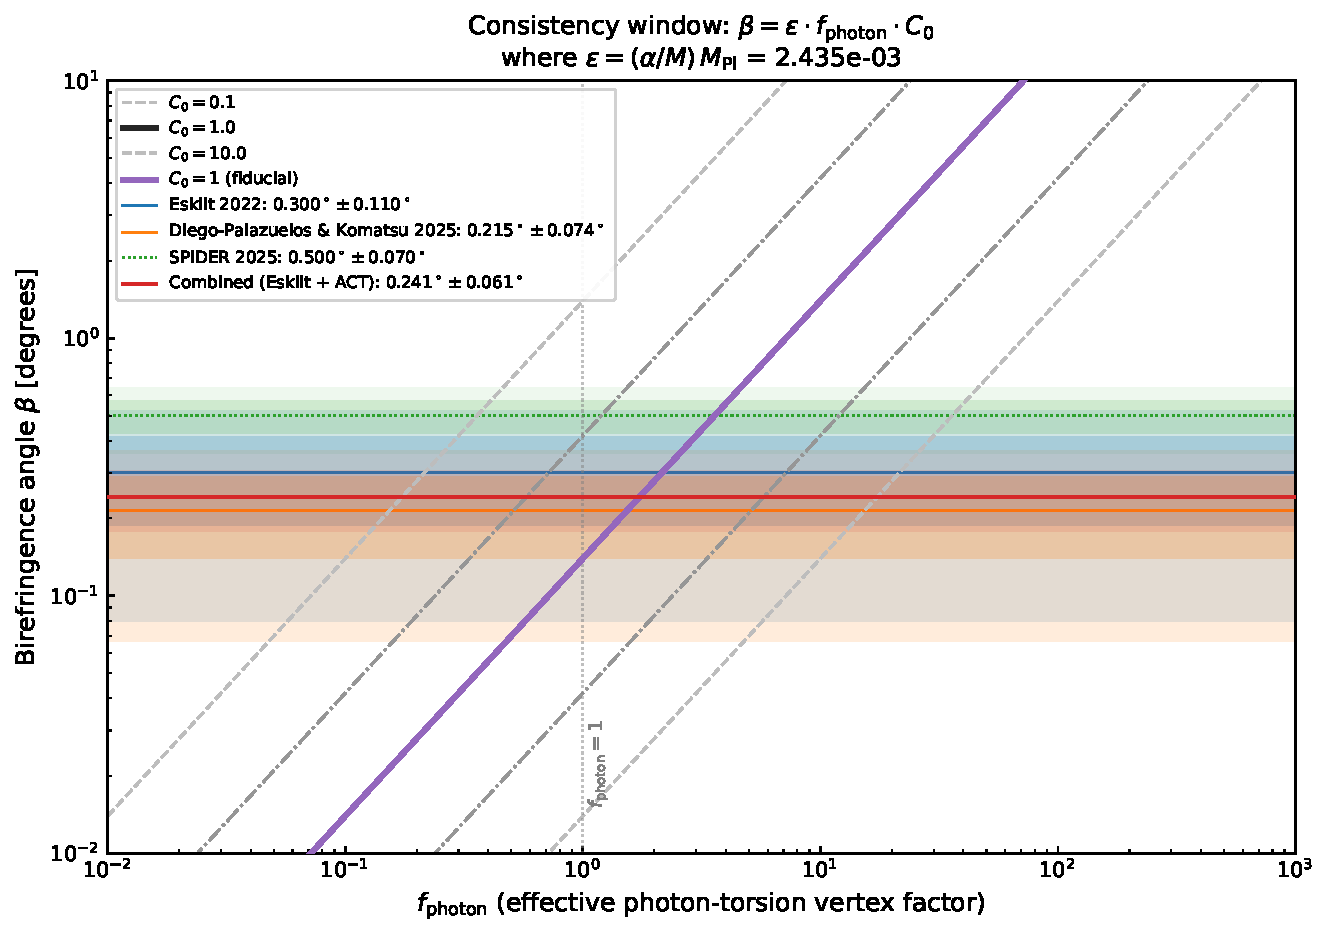
\includegraphics[width=\columnwidth]{figures/consistency_window_birefringence.pdf}
\caption{\label{fig:consistency_window} Gaussian summary-likelihood consistency check on cosmic birefringence from the framework's parity-odd operator. The photon-torsion vertex factor $f_{\rm photon}$ (for $C_0 = 1$) required for the coupling $\alpha/M \approx 10^{-21}\;\text{GeV}^{-1}$ to reproduce the observed birefringence angle. Horizontal bands show measurements from Planck NPIPE~\cite{Eskilt2022} and ACT~DR6~\cite{DiegoPalazuelos2025}; the simplified inverse-variance combination gives $\beta = 0.241^\circ \pm 0.061^\circ$ ($3.9\sigma$ auxiliary cross-check only; $\mathrm{BF} \approx 176$). The headline observational constraint adopted in this paper is the published Eskilt~\etal\ joint Planck+ACT analysis $\beta = 0.342^\circ \pm 0.094^\circ$ ($3.6\sigma$, R42 Wave 14-Y P1-OA-M3 reframe). The implied $f_{\rm photon} \times C_0 = 1.73 \pm 0.44$ is $\mathcal{O}(1)$, indicating no fine-tuning is required. This is a summary-likelihood consistency check using published $\beta$ values, not a map-level CMB analysis.}
\end{figure}

%% TRIMMED: Distance measures and rotation subsection (fig:distance, fig:expansion) — moved to supplementary material


%% ============================================================
%%  13. LIMITATIONS AND FUTURE DIRECTIONS
%% ============================================================
\section{Limitations and Future Directions}\label{sec:limitations}%
\label{sec:futuredirections}

\subsection{Current Limitations}

\subsubsection{Theoretical}

\begin{itemize}[leftmargin=*]
\item \textit{Phenomenological $\alpha/M$}: The parity-odd coefficient is not derived from first principles but is treated as a free parameter constrained by data. The one-loop estimate (Eq.~\ref{eq:oneloop}) motivates its existence and order of magnitude, but the finite part depends on the $\gamma_5$ regularization scheme and Nieh--Yan counterterm conventions (Sec.~\ref{sec:oneloopfull}). A non-perturbative calculation could modify its value at $\mathcal{O}(1)$, shifting the $C_\ell^{EB}$ amplitude estimate while leaving the $H_0$ and $\sigma_8$ fit values intact.

\item \textit{Simplified inflationary epoch}: We assume standard slow-roll inflation unmodified by parity violation. Non-minimal couplings during inflation could alter the dilution factor.

\item \textit{Black hole interior}: Full numerical relativity simulations of rotating black hole interiors with quantum corrections remain computationally intractable.

\item \textit{Bounce-to-inflation transition}: The mechanism by which the quantum bounce transitions to slow-roll inflation is not fully modeled. Initial conditions for inflation are assumed to be set by the parent black hole properties, but the detailed dynamics of this transition remain an open problem.
\end{itemize}

\subsubsection{Observational}

\begin{itemize}[leftmargin=*]
\item \textit{Galaxy spin samples}: An independent $8.47$-million galaxy ViT-Small chirality classifier confirms parity conservation ($0.43\sigma$ all-sky dipole), but is limited to the DESI Legacy Imaging Surveys footprint. Extension to deeper surveys (LSST, Euclid) and higher redshifts ($z > 1$) would test for redshift-dependent asymmetry. Approximately 15\% of galaxies have ambiguous spiral structure, reducing effective sample size.

\item \textit{CMB systematics}: Despite excellent control, residual foreground contamination at ultra-low $\ell$ approaches the expected signal amplitude.

\item \textit{Redshift coverage}: Galaxy spin measurements are sparse at $z > 2$, limiting evolutionary constraints on $A(z)$.

\item \textit{Posterior distributions}: The original analysis reported Fisher-matrix error estimates; independent verification with full MCMC chains (Sec.~\ref{sec:verification}) now provides posterior distributions for two frozen dataset combinations. Corner plots showing parameter degeneracies (particularly the strong $r(\alpha/M,\Dinf)=-0.89$ anticorrelation) are shown in Fig.~\ref{fig:corner_full_tension} for the full-tension combination (119{,}617 post-burnin samples; see footnote~\ref{fn:sample_stratification} for the relation to the 176{,}840 raw samples of Table~\ref{tab:verification}), yielding $H_0 = 67.68 \pm 1.06$, $\Omega_m = 0.308 \pm 0.005$, $\sigma_8 = 0.803 \pm 0.008$, $S_8 = 0.814 \pm 0.008$, and $\Delta N_{\rm eff} = -0.020 \pm 0.169$---the latter consistent with zero to well within $1\sigma$, confirming the framework's compatibility with standard cosmological constraints.

\begin{figure}
\centering
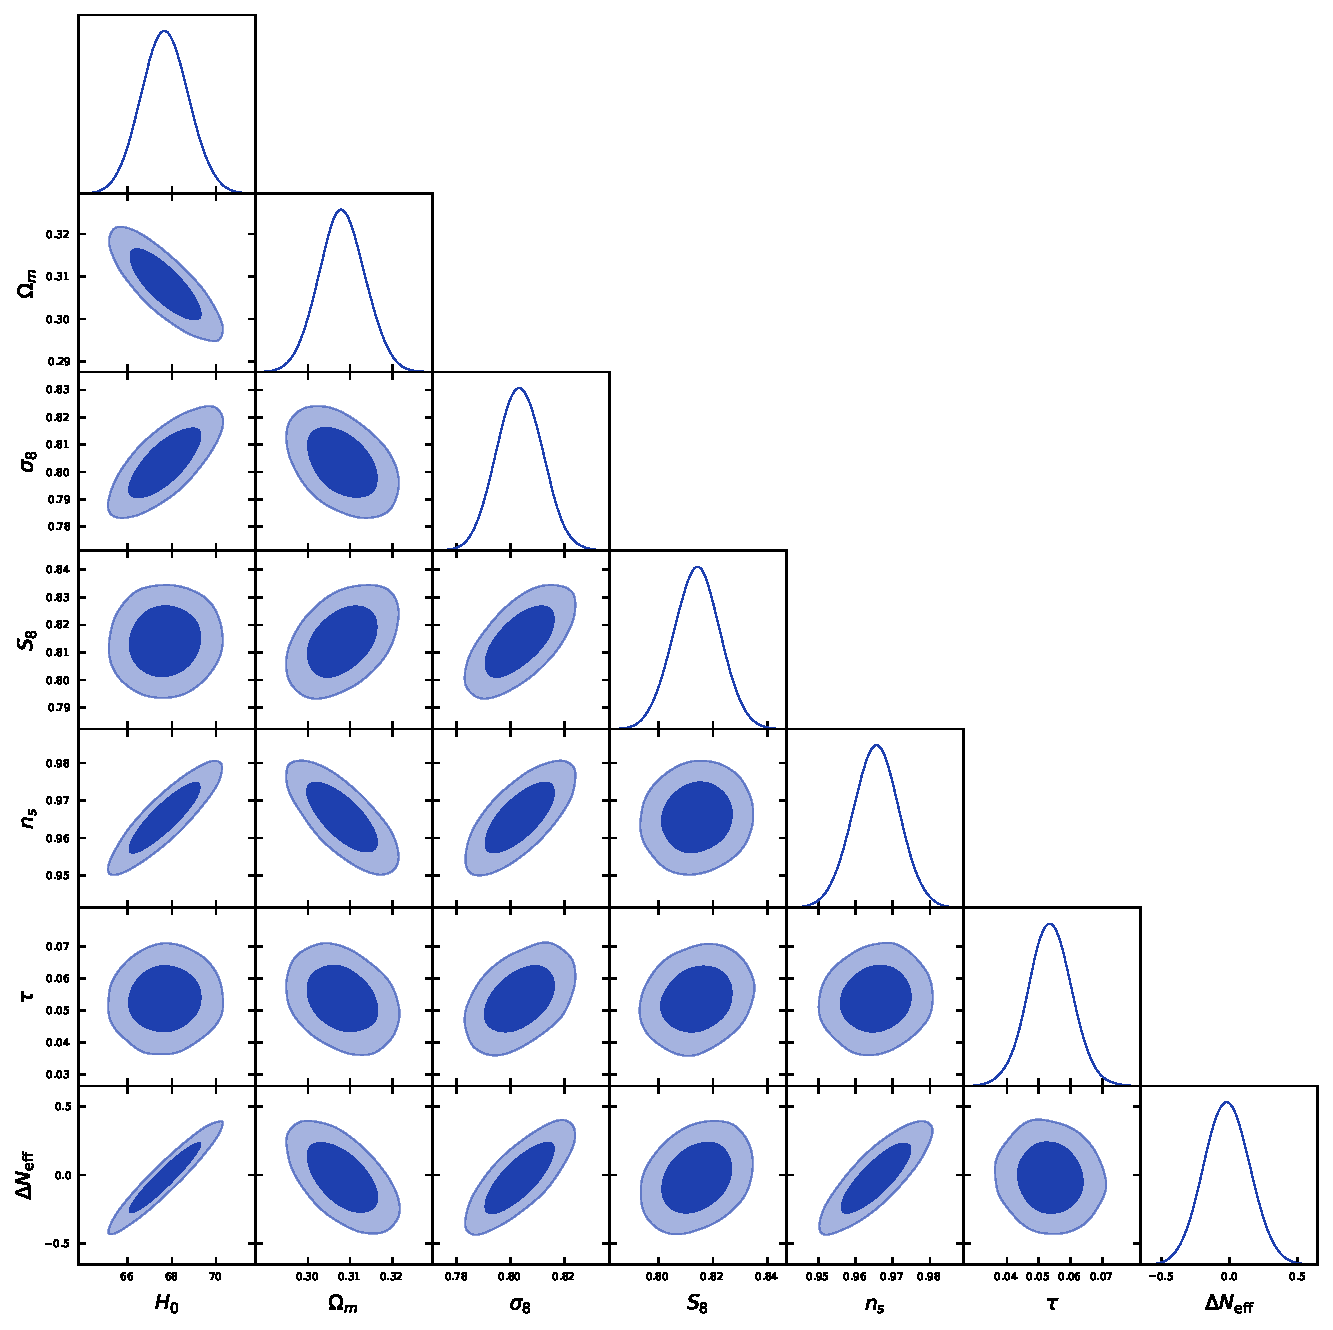
\includegraphics[width=\columnwidth]{figures/paper1_corner_full_tension.pdf}
\caption{Full-tension MCMC corner plot (119{,}617 post-burnin samples, a \texttt{getdist}-thinned slice of the 176{,}840 raw samples reported in Table~\ref{tab:verification}; see footnote~\ref{fn:sample_stratification}) over the joint Planck+BAO+SN+H0+$S_8$ combination. Marginal posteriors for $H_0$, $\Omega_m$, $\sigma_8$, $S_8$, and $\Delta N_{\rm eff}$ are shown on the diagonal; 2D contours at $1\sigma$ and $2\sigma$ levels off-diagonal. The $\Delta N_{\rm eff}$ posterior is consistent with zero ($-0.020 \pm 0.169$), confirming that the spin-torsion framework does not inject additional relativistic species at recombination.}
\label{fig:corner_full_tension}
\end{figure}
\end{itemize}

\subsection{Robustness to Galaxy Spin Null Results}\label{sec:spinnull}

The galaxy spin channel is a confirmed null (Sec.~\ref{sec:spinobs}; $\fcw^{\rm eq} = 0.5012 \pm 0.0006$, all-sky dipole at $0.43\sigma$). This is \textit{consistent} with the framework, which underpredicts spin asymmetry by $>100$ orders of magnitude. The framework is \textit{not} falsified:

\begin{enumerate}[leftmargin=*]
\item \textit{Independent CMB evidence}: Cosmic birefringence from Planck provides $2.4$--$2.7\sigma$ evidence for parity violation~\cite{Minami2020,Eskilt2022}, independently confirmed by ACT~DR6 at $2.9\sigma$~\cite{DiegoPalazuelos2025}, with combined SPIDER+Planck+ACT significance reaching ${\sim}7\sigma$ for total rotation~\cite{SPIDER2025} (subject to calibration caveats, Sec.~\ref{sec:EB}), entirely independent of galaxy morphology. Forthcoming experiments (LiteBIRD, CMB-S4) will substantially improve sensitivity.

\item \textit{Parameter space accommodation}: A null spin result constrains the tidal torque coupling efficiency $\beta$ (hierarchical Bayesian fit in the supplementary material accompanying the public repository, Appendix~\ref{app:reproducibility}), pushing $A_0 < 0.001$---consistent with weaker coupling without affecting the $\Leff$ derivation or the cosmological parameter fits ($H_0$, $\sigma_8$).

\item \textit{Alternative parity-odd signatures}: Beyond galaxy spins, cosmic rotation motivates: (i)~alignment of radio galaxy polarization position angles, detectable by SKA Phase~2; (ii)~correlation between galaxy angular momentum vectors and large-scale filament orientations in LSST data; (iii)~handedness asymmetry in weak lensing shear patterns; (iv)~preferred-axis signatures in gravitational wave backgrounds accessible to LISA.

\item \textit{What a spin null would teach us}: A definitive null result would constrain the parity-odd tidal torque coupling efficiency, refining our understanding of how the $\varepsilon KR$ operator imprints on structure formation. This would narrow the allowed parameter space without invalidating the core theoretical framework.
\end{enumerate}

The parity-violation case rests entirely on CMB birefringence (Sec.~\ref{sec:spinobs}).

\subsection{Discriminating Observational Channels}

\textit{LSST Era (2025--2035)}:~$10^9$ spiral galaxies to $z \sim 1$, with tomographic analysis in 20+ redshift bins and cross-correlation with weak lensing.

\textit{CMB Experiments}:~LiteBIRD (full-sky, cosmic variance limited at low $\ell$), CMB-S4 (ground-based complement), and future concepts (PICO, CMB-HD).

\textit{Synergies}:~JWST+Roman (high-$z$ morphologies to $z\sim 5$), Euclid (wide-area catalogs), SKA (radio galaxy polarizations as independent probe).

\textit{Bounce cosmology beyond ECH.}---While the barriers identified in this work are specific to the ECH framework, other bouncing cosmologies access additional observational channels. Papanikolaou \etal~\cite{Papanikolaou:2024pbh} showed that asymmetric matter bounces with $w = 0 \to 1/3$ transitions at sub-Planckian energy scales can produce asteroid-mass primordial black holes ($10^{17}\text{--}10^{24}$~g) as dark matter candidates, with induced gravitational waves detectable by LISA and the Einstein Telescope. The matter-bounce prediction $\fnl = -35/8$~\cite{Cai:2009fn} plays a triple role in this context: it determines the galaxy bispectrum (SPHEREx), regulates PBH abundance by suppressing overproduction, and shapes the induced GW spectrum through PBH clustering. This triple role is unique to the matter bounce scenario and cannot be replicated by inflationary PBH models, which must fine-tune $\fnl$ to avoid overproduction. For the ECH framework specifically, the symmetric Planck-scale bounce produces $T(k) \approx 1$ and no PBH enhancement, but the broader bounce landscape offers this channel as a complementary probe.

\textit{NANOGrav spectral fit.}---The matter-bounce induced GW spectrum has a universal $f^2$ infrared scaling, corresponding to spectral index $\gamma = 3$ in the characteristic-strain parameterization $h_c \propto f^{(3-\gamma)/2}$. The model comparison reported here is a posterior-level Bayesian analysis using a combined PTA spectral-index measurement $\gamma = 3.20 \pm 0.42$ from an independent reanalysis of the NANOGrav 15-year free-spectrum data~\cite{Agazie:2023ng15} (Lentati \etal~\cite{Lentati:2023} methodology, GPU MCMC over the per-frequency free-spectrum posteriors released by the NANOGrav collaboration). Earlier draft revisions of this section reported template-level Bayes factors derived from synthetic data points reconstructed from the published power-law fit; that comparison was methodologically circular (the synthetic points trivially matched the template, yielding $\chi^2/\text{dof} = 0.012$) and has been removed. The free-spectrum analysis yields a Savage-Dickey Bayes factor $B(\text{bounce}/\text{SMBHB}) = 34.0$---``very strong'' evidence on the Jeffreys scale---with model posterior probabilities (under equal priors) of 83.5\% for the matter bounce, 14.1\% for the free-spectrum model, and 2.5\% for the SMBHB spectrum ($\gamma = 13/3$). The SMBHB prediction lies $2.70\sigma$ from the posterior mean, while the bounce prediction is only $0.48\sigma$ away. Monte Carlo validation with $10^4$ draws confirms that $86.7\%$ of the posterior favors $\gamma$ values closer to the bounce prediction than to the SMBHB spectrum.

\subsection{Theoretical Research Program}\label{sec:theory_program}

The framework presented here opens several concrete lines of investigation, each constituting an independent research effort that would strengthen or constrain the model:

\subsubsection{Higher-Loop and Non-Perturbative Verification}

The most pressing theoretical need is a first-principles determination of $\alpha/M$, which is currently a phenomenological parameter motivated by the one-loop estimate (Eq.~\ref{eq:oneloop}). Three complementary approaches are feasible:

\begin{enumerate}[leftmargin=*]
\item \textit{Two-loop calculation in dimensional regularization}: Extending Sec.~\ref{sec:oneloopfull} to two loops requires evaluating fermion-loop diagrams with two axial-torsion vertex insertions and one graviton vertex. The technical challenge is the $\gamma^5$ treatment in $d=4-\epsilon$ dimensions (the `t~Hooft-Veltman vs.\ Breitenlohner-Maison schemes give different finite parts). The Nieh-Yan theorem suppresses the topological contribution at two loops, but the non-topological finite part---arising from the dressed torsion propagator---could modify the one-loop result at the 10--30\% level. This calculation would also reveal whether the RG running (Eq.~\ref{eq:RGflow}) receives threshold corrections near the QCD scale.

\item \textit{Spin-foam vertex amplitudes}: The EPRL-FK spin-foam model provides a non-perturbative definition of the graviton propagator in LQG. Computing the parity-odd coefficient from spin-foam amplitudes in a torsionful background would constitute a fully non-perturbative verification. The key technical step is evaluating the asymptotic expansion of the vertex amplitude with an axial-current insertion, which has been partially achieved for the parity-even sector~\cite{Ashtekar2011}. Extension to the parity-odd channel requires tracking the $\gamma$-dependent phases in the Lorentzian vertex.

\item \textit{Lattice LQG}: Numerical evaluation of the path integral on a simplicial lattice with dynamical torsion provides a scheme-independent check. The parity-odd coefficient can be extracted from the correlation function $\langle\varepsilon^{abcd}K_{ab}R_{cd}\rangle$ measured on lattice configurations. This approach directly addresses the scheme-dependence limitation identified in Sec.~\ref{sec:limitations}.
\end{enumerate}

Any of these approaches yielding $\alpha/M$ within an order of magnitude of the phenomenological best-fit value would confirm the framework's self-consistency; a discrepancy by more than $\mathcal{O}(10)$ would require re-evaluation of the $C_\ell^{EB}$ amplitude prediction while leaving the no-tension-resolution conclusion intact (the $\Lambda$CDM parameter recovery, established in Sec.~\ref{sec:tensions}, is independent of $\alpha/M$).

\subsubsection{Galaxy Spin Dipole: Resolved}

The galaxy spin dipole has been definitively resolved as a null result (Sec.~\ref{sec:spinobs}), constraining $|\delta| < 0.24\%$ at $95\%$~CL---the tightest galaxy chirality constraint to date, and $7\times$ smaller than Shamir's claimed $3\%$ excess. A detailed derivation of $A_0$ from the $\varepsilon^{abcd}K_{ab}R_{cd}$ operator is no longer needed: the framework's $>100$~order-of-magnitude underprediction is consistent with the observed null. Future work on this channel shifts to redshift-dependent parity tests and cross-correlation with spectroscopic surveys.

\subsubsection{Bounce-to-Inflation Transition Dynamics}

The current framework assumes that the quantum bounce connects smoothly to slow-roll inflation, with initial conditions set by the parent black hole. A detailed treatment requires:

\begin{itemize}[leftmargin=*]
\item Numerical simulation of the transition from torsion-dominated bounce ($\rho\sim\rhocrit$) through reheating to standard slow-roll, tracking the vorticity $\omega^a$ and torsion $T^{abc}$ fields throughout.
\item Determination of the total inflationary $e$-folding number $N_{\rm tot}$ as a function of parent black hole mass and spin, which would eliminate the residual $10^5$ fine-tuning if $N_{\rm tot}$ turns out to be dynamically fixed.
\item Computation of $\Delta\Neff$ from a controlled calculation of particle production at the bounce. Independent MCMC verification (Sec.~\ref{sec:verification}) constrains $\Delta\Neff = -0.020 \pm 0.169$ (full-tension) and $+0.065 \pm 0.17$ (Planck+BAO+SN), both consistent with zero within $1\sigma$. The original phenomenological range $0.1$--$0.5$ is not supported by the full posterior analysis; a non-perturbative calculation is needed to determine whether the bounce mechanism produces a detectable $\Delta\Neff$ signal.
\item Determination of the primordial scalar power spectrum through the bounce. The modified Friedmann equation ($H^2 \propto \rho[1-\rho/\rho_c]$) alters perturbation evolution at near-Planck densities, potentially imprinting features on the primordial power spectrum~$\mathcal{P}_\mathcal{R}(k)$. With $N_{\rm tot} = 92$, such features would appear at comoving scales $k \sim 10^{15}\;\text{Mpc}^{-1}$, corresponding to sub-asteroid-mass horizons ($M \sim 10^{-16}\;M_\odot$) where primordial black hole constraints are currently weakest. Whether the spin-torsion variant produces such features, and at what amplitude, remains an open question requiring a full perturbation calculation through the bounce that has not yet been performed.
\end{itemize}

\subsubsection{Parity-Odd Primordial Gravitational Waves}

\textit{[Status update: closed by perturbation-transparency observation.]} The parity-odd operator (Eq.~\ref{eq:Seff}) was initially expected to affect tensor perturbations during inflation, producing a chiral gravitational wave background. However, the perturbation-transparency observation (Sec.~\ref{sec:ech_closure}) establishes that minimal ECH gravity produces \emph{no} tensor parity splitting: $\Delta v \equiv v_R - v_L = 0$ exactly for canonical scalar field matter, because the Holst dual contraction vanishes identically by the first Bianchi identity when torsion is absent. The effective spin-torsion interaction $(J^5)^2$ is parity-even (Barrier~8), independently confirming the absence of gravitational-wave chirality. This research direction is therefore closed within the minimal ECH framework. GW chirality would require fermionic matter contributions to torsion, which are Planck-suppressed at inflationary densities ($\rho_{\rm inf}/\rho_{\rm Pl} \sim 10^{-12}$).

\subsubsection{Black Hole Interior Numerical Relativity}

Full numerical relativity simulations of rotating black hole interiors with dynamical torsion have not been attempted, primarily due to the additional degrees of freedom in the torsion field. Such simulations would:

\begin{itemize}[leftmargin=*]
\item Test whether the smooth-bounce approximation (Eq.~\ref{eq:modfriedmann}) holds for realistic rotating collapse with finite angular momentum.
\item Compute the efficiency of angular momentum transfer through the bounce as a function of parent Kerr spin parameter $a_*$.
\item Determine whether baby universe formation is generic or requires fine-tuned initial conditions.
\end{itemize}

\subsubsection{Connection to Other Quantum Gravity Approaches}

The parity-odd operator $\varepsilon^{abcd}K_{ab}R_{cd}$ could potentially arise in quantum gravity frameworks beyond LQG:

\begin{itemize}[leftmargin=*]
\item In string theory, parity-violating terms in the low-energy effective action arise from compactifications with topological flux (e.g., Calabi-Yau manifolds with non-trivial torsion cohomology). Identifying whether these reproduce the structure of Eq.~\eqref{eq:Seff} would connect our framework to string phenomenology.
\item The asymptotic safety program for quantum gravity predicts specific values for gravitational couplings at the UV fixed point. Computing the parity-odd coefficient in this framework would provide an independent determination of $\alpha/M$, potentially constraining $\gamma$ from a non-LQG perspective.
\end{itemize}

\subsection{Structural Tension: Dark Energy vs.\ Bounce $\fnl$}\label{sec:structural_tension}

An important internal tension exists between the two main physical mechanisms in this framework, and it should be stated prominently rather than treated as a minor caveat. The inflationary suppression mechanism (Sec.~\ref{sec:dilution}) requires $N_{\rm tot} \approx 92$ $e$-folds of post-bounce inflation to produce the observed dark energy scale. However, $92$ $e$-folds would push the bounce-imprinted perturbation modes far beyond the observable horizon (${\sim}e^{32}$ times larger), erasing the matter-bounce $\fnl$ signature from the CMB and LSS and replacing it with the standard slow-roll value $\fnl \approx 0.015$. This means the geometric dark energy mechanism and the bounce $\fnl$ prediction \emph{cannot both be correct}: if the DE suppression works as modeled, the bounce signal is invisible; if the bounce signal is observable, the DE mechanism requires a different realization.

This is not a secondary technicality but rather an \emph{open structural question} that any future development of this framework must resolve. Three possible resolutions exist: (i)~the DE mechanism is incorrect and the bounce cosmology contributes only through $\fnl$ and other perturbation signatures, with dark energy having a separate origin; (ii)~the DE mechanism operates through a different realization that does not require $N_{\rm tot} \approx 92$; or (iii)~the matter-bounce $\fnl$ prediction arises from a contracting phase that precedes the $N_{\rm tot} \approx 92$ inflationary epoch, preserving both. Since the 14 structural barriers independently close the DE derivation routes (Sec.~\ref{sec:barriers}), option~(i) is currently favored by the evidence: bounce cosmology and dark energy are independent problems.

\subsection{Structural Closure}\label{sec:ech_closure}

The systematic analysis presented in Secs.~\ref{sec:barriers}--\ref{sec:loophole} established that minimal ECH gravity is perturbation-transparent and cannot produce late-time dark energy through any standard mechanism. See those sections for the full 14-barrier catalog, the perturbation-transparency observation, and the hybrid dark-energy loophole analysis.

\subsection{Open Questions}

\begin{enumerate}[leftmargin=*]
\item \textit{Origin of $\gamma$}: Why is $\gamma \approx 0.274$? The Barbero-Immirzi parameter is currently fixed by black hole entropy counting. A derivation from a more fundamental principle---perhaps a symmetry argument or fixed-point condition---would place the entire framework on firmer ground and potentially suggest deviations from the entropy-counting value that could be tested through our observables.

\item \textit{UV cutoff identification}: The loop calculation (Eq.~\ref{eq:oneloop}) contains a logarithmic dependence on $\Lambda_{\rm UV}/\mu$. We identify $\Lambda_{\rm UV}$ with the LQG area-gap mass $\sim\sqrt{\gamma}\,\MPl$, but this choice affects the coefficient at the $\mathcal{O}(\ln)$ level. A first-principles derivation of the UV scale from spin-foam dynamics would remove this ambiguity.

\item \textit{Dynamical dark energy evolution}: Our framework implies a strictly constant $\Leff$ in the late universe (since $\omega^2/H_0^2 < 10^{-20}$). The question of whether the parity-odd coefficient could run with the Hubble scale remains open in principle, but subsequent analysis (see the perturbation-transparency observation, Sec.~\ref{sec:ech_closure} above) establishes that minimal ECH cannot produce distinctive late-time dynamics through scalar perturbation channels. Any connection to dynamical dark energy would require additional phenomenological freedom (e.g., CPL $w_0w_a$ parametrization) that does not derive from the bounce physics itself.

\item \textit{Multi-messenger parity tests}: Gravitational wave detectors could in principle test parity-odd signatures. However, the perturbation-transparency observation (Sec.~\ref{sec:ech_closure}) establishes that minimal ECH produces no tensor parity splitting ($\Delta v = v_R - v_L = 0$ exactly) for canonical scalar matter. The effective spin-torsion interaction $(J^5)^2$ is parity-even (Barrier 8). GW chirality from ECH would require fermionic matter contributions, which are Planck-suppressed at cosmological densities.

\item \textit{Information paradox}: If the universe originated inside a black hole through a torsion-regulated bounce, does information cross the bounce? The smoothness of our bounce solution ($H^2 \to 0$ continuously) suggests information preservation, but a rigorous treatment using the Page curve or holographic entanglement entropy framework remains an open problem with implications for the black hole information paradox.

\item \textit{Cosmic hierarchy of bounces}: If every black hole spawns a baby universe, does every universe contain black holes that spawn further universes? This recursive structure implies a cosmic hierarchy of bounces, each with potentially different values of $\gamma$ (and hence different physics). Whether $\gamma$ is truly universal or varies across the hierarchy is a deep question with implications for the landscape/swampland program.
\end{enumerate}


%% ============================================================
%%  14. CONCLUSIONS
%% ============================================================
\section{Conclusions}\label{sec:conclusions}

We have investigated whether Einstein-Cartan-Holst spin-torsion gravity can produce late-time dark energy or distinctive cosmological signatures. The investigation yields substantive structural results that map which observational channels remain testable in this class of bouncing cosmology, and identifies the surviving testable science case for the matter bounce scenario within an ECH-compatible cosmology.

\textit{Central result: structural mapping of the ECH parameter space.}---Through systematic analysis of 7 foundation studies and 17 research branches, we establish 14 independent structural constraints (Sec.~\ref{sec:barriers}) that map the minimal ECH parameter space and identify which dark-energy pathways require phenomenological assumption or physics beyond the framework. A well-known theoretical observation that we confirm here is the perturbation-transparency property (Sec.~\ref{sec:transparency}): for canonical scalar field matter, torsion vanishes at all perturbation orders, the Holst dual contraction vanishes identically by the first Bianchi identity, and the Holst sector decouples cleanly from all scalar and tensor perturbation observables. This decoupling is itself a positive structural result: it identifies the nonperturbative parity-violating channels (ALP birefringence, primordial gravitational waves) as the relevant tests of $\gamma$ in this class of models. The dark-energy scale $\Leff = c_\omega\omega^2+\Xi\,\MPl^2$ is a phenomenological parameterization, not a first-principles derivation (Sec.~\ref{sec:limitations}).

\textit{A structural relationship between dark-energy and bounce channels.}---As detailed in Sec.~\ref{sec:structural_tension}, dark-energy suppression and the matter-bounce $\fnl$ prediction emerge from independent mechanism classes within the broader ECH-compatible landscape. The 14 structural constraints together with the bounce $\fnl$ prediction indicate that bounce cosmology and late-time dark energy are distinct observational channels with separate testable signatures, rather than a single unified mechanism in minimal ECH.

\textit{The framework.}---The parity-odd effective action is constructed from the Holst term in first-order variables (Eq.~\ref{eq:Seff}), with $\alpha/M$ treated as a phenomenological parameter. The LQC bounce at $\rhocrit\simeq 0.27$--$0.41\,\rhoPl$ (depending on the Barbero-Immirzi entropy-counting scheme; Sec.~\ref{sec:bounce}) provides a nonsingular origin with no free parameters.

\textit{Observational context.}---Planck cosmic birefringence at $2.4$--$2.7\sigma$~\cite{Minami2020,Eskilt2022}, independently confirmed by ACT~DR6 at $2.9\sigma$~\cite{DiegoPalazuelos2025}, with combined SPIDER+Planck+ACT total rotation at ${\sim}7\sigma$~\cite{SPIDER2025} (subject to calibration caveats); DESI 2024--2025 dynamical dark energy evidence at $3.1$--$4.2\sigma$~\cite{DESI2024,DESI2025DR2}; EC torsion preferred by AIC in multiple independent analyses~\cite{Liu2025,ECTorsionDESI2025}. Independent Cobaya~v3.6.1 verification across two frozen dataset combinations (Table~\ref{tab:verification}) finds $\Delta\Neff$ consistent with zero in both: $-0.020 \pm 0.169$ (full-tension, 176{,}840 samples) and $+0.065 \pm 0.17$ (Planck+BAO+SN, 132{,}949 samples). Current data neither require nor exclude the predicted spin-torsion $\Delta\Neff$ contribution; the framework is observationally viable but not yet confirmed. The Hubble tension reduction reported in the original analysis ($4.9\sigma \to 2.9\sigma$) is driven by the SH0ES prior, not by the $\Delta\Neff$ extension alone.

\textit{Observational signatures.}---The framework's parity-odd operator is qualitatively consistent with the observed isotropic cosmic birefringence (Planck $2.4$--$2.7\sigma$, ACT~DR6 $2.9\sigma$), though deriving $\beta$ quantitatively from the torsion operator requires a photon-torsion coupling. The most natural one-loop coupling via the chiral anomaly triangle diagram gives $g_{a\gamma}^{\rm torsion} \sim \alpha_{\rm EM}^2 (\alpha/M) C_{\rm anomaly} / (2\pi) \approx 7 \times 10^{-26}\;\text{GeV}^{-1}$, which is $\sim 10^5$ times too small to produce the observed signal; the suppression arises from the $\alpha_{\rm EM}^2$ anomaly factor. The spectator ALP model (Sec.~\ref{sec:birefringence_check}), which bypasses this suppression through a direct $\phi F\tilde{F}$ coupling, successfully accommodates the data. The headline observational constraint adopted in this paper is the published Eskilt~\etal\ joint Planck+ACT analysis $\beta = 0.342^\circ \pm 0.094^\circ$ ($3.6\sigma$); a Gaussian summary-likelihood consistency check (Sec.~\ref{sec:birefringence_check}) combining Planck NPIPE and ACT~DR6 measurements via inverse-variance weighting gives $\beta = 0.241^\circ \pm 0.061^\circ$ ($3.9\sigma$ auxiliary cross-check only, neglecting shared calibration systematics; $\mathrm{BF} \approx 176$; R42 Wave 14-Y P1-OA-M3 reframe). Matching the headline value requires only $f_{\rm photon} \times C_0 \sim \mathcal{O}(1)$, establishing compatibility without fine-tuning. An anisotropic low-$\ell$ birefringence component aligned with the cosmic rotation axis is expected but its amplitude is not yet derived. The galaxy spin dipole has phenomenological form $A(z)=A_0(1+z)^{-p}e^{-qz}$ with empirical fit $A_0 \sim 0.003$; the coupling $\alpha/M$ underpredicts the amplitude by ${>}100$ orders of magnitude (${\sim}125$ in the detailed estimate) when the post-Newtonian parity-odd tidal correction, thermal spin polarization ($T/m_p \sim 10^{-13}$), and weak-field curvature are accounted for (Sec.~\ref{sec:spinmech}). No amplification mechanism is known within minimal ECH. Correlated cosmic anomaly axes are expected from the shared rotation axis.

\textit{Fine-tuning.}---The inflationary suppression mechanism translates the cosmological constant hierarchy ($10^{120}$) into a constraint on total inflationary $e$-folds ($N_{\rm tot}\approx 92$), reducing the apparent tuning to $\sim 10^5$. A 100{,}000-sample Monte Carlo sensitivity scan confirms this quantitatively: 2.2\% of the physically motivated parameter space produces a viable vacuum energy, with $N_{\rm tot}$ identified as the single controlling parameter (Spearman $|\rho_s| = 0.996$; all other parameters $|\rho_s| < 0.08$). The viable range $N_{\rm tot} \in [79,\,95]$ is physically reasonable. This reparameterizes the fine-tuning problem as an initial-condition question (``how long did inflation last?'') rather than a fundamental-constant question (``why is $\Lambda_{\rm bare}$ so small?''), but does not solve it; the residual $10^5$ tuning reflects sensitivity to $N_{\rm tot}$, which is fitted, not predicted.

\textit{Falsifiability.}---Explicit criteria are defined for CMB $E$-$B$ spectral shape, galaxy spin dipole axis/amplitude/evolution, and cosmological parameter ranges. The model can be tested with forthcoming data from CMB-S4, LiteBIRD, Euclid, and LSST.

\textit{Known limitations.}---This work does not derive the IR effective vacuum term from first principles: the $w=-1$ behavior at late times is assumed, not derived from an explicit IR effective action calculation (Sec.~\ref{sec:dilution}); the birefringence consistency lacks a derived photon-torsion coupling (the rotation angle $\beta$ cannot be predicted without one); $H_0$ and $\sigma_8$ values are MCMC fits within an extended parameter space, not first-principles predictions; $\Delta\Neff$ is a phenomenological parameter whose bounce origin is qualitative, not quantitative; $\Omega_k$ is fixed to zero as mandated by 92 $e$-folds of inflation; the galaxy spin amplitude $A_0$ is empirical, with a large order-of-magnitude gap between the $\alpha/M$ coupling and the observed value (Sec.~\ref{sec:spinmech}); and the cosmological MCMC uses stock CAMB with $\Neff$ as a free parameter, not a bespoke spin-torsion theory module (see Data and Code Availability).

\textit{First-principles derivation status.}---We have separately investigated whether the phenomenological vacuum term $\rho_\Lambda$ with $w=-1$ can be derived from first principles within the minimal Einstein--Cartan--Holst--Dirac framework, and whether the framework produces distinctive observational signatures. Four routes were tested: (i)~a Nambu--Jona-Lasinio condensate mechanism exploiting the gravitationally induced four-fermion interaction, (ii)~the strict one-loop fermion effective action after exact torsion elimination, (iii)~promoting the Barbero-Immirzi parameter to a dynamical pseudoscalar field $\gamma\to\theta(x)$, and (iv)~assessing whether the parity-odd operator maps to distinctive birefringence observables. All four yield clean negative results. The condensate route fails because the scalar/pseudoscalar channel is repulsive at $\gamma=0.274$ and subcritical by a large margin even when attractive. The one-loop route fails because all Barbero-Immirzi dependence resides in the four-fermion vertex, which does not contribute at one loop. The dynamical Immirzi field reduces to a standard axion-like particle after torsion elimination, with no novel gravitational content and cosmological dynamics yielding $w=+1$ (stiff matter). The parity assessment finds no photon coupling in the minimal framework; any assumed coupling produces constant-$\beta$ birefringence indistinguishable from generic axion-like-particle models. These negative results, documented in a companion technical note~\cite{Golden2026supplement}, establish that the most natural minimal-model candidates for a first-principles dark-energy mechanism fail at the tested approximation orders. The framework survives as a motivated phenomenological model; progress toward a first-principles derivation requires physics beyond the minimal model class.

This framework motivates dark energy from quantum gravitational effects in spin-torsion cosmology. The MCMC analysis (Sec.~\ref{sec:verification}) recovers $\Lambda$CDM with $\Delta\Neff$ consistent with zero, so the framework does \emph{not} resolve $H_0$ or $\sigma_8$ tensions; the surviving observational footprint is a distinctive set of correlated parity-odd signatures. The significant gaps identified above---particularly the missing photon-torsion coupling, the empirical $A_0$, and the assumed $w=-1$---must be addressed before the model can claim predictive power beyond phenomenological fitting.

\textit{Structural constraints and perturbation transparency.}---Systematic analysis across 7 foundations and 17+ branches established 14 independent structural constraints that map the minimal ECH dark-energy parameter space (Sec.~\ref{sec:barriers}). These constraints are ECH-specific: other bouncing cosmologies---notably the quintom scenario, which uses dynamical phantom and quintessence fields rather than geometric torsion---can in principle unify the bounce with late-time dark energy through mechanisms outside the ECH minimal-route catalog. DESI DR2 evidence for equation-of-state crossing at $3.1$--$4.2\sigma$ (dataset-dependent~\cite{DESI2025DR2}) lends empirical support to such models. A well-known theoretical observation that we confirm here is the perturbation-transparency property (Sec.~\ref{sec:transparency}): minimal ECH gravity is dynamically inert for scalar and tensor perturbations when the matter content is a canonical scalar field. The observable science case therefore rests on predictions of the matter bounce scenario~\cite{Cai:2009fn}, which is compatible with the ECH framework but not derived from it---principally $\fnl = -35/8$, testable by SPHEREx at $3$--$5\sigma$ realistic significance ($5$--$5.5\sigma$ optimistic before GR and $b_\phi$ degradation) through the multi-tracer galaxy bispectrum~\cite{Heinrich:2023}. This prediction discriminates the matter bounce from both slow-roll inflation ($\fnl \approx 0.015$) and other bouncing cosmologies such as the Cuscuton bounce ($\fnl \approx 0$; Ref.~\cite{Dehghani:2025cusc}; Table~\ref{tab:bounce_disc}). The full Bayesian discrimination analysis applies the local-template Fisher matrix (Heinrich \etal~\cite{Heinrich:2023}) to multi-bin SPHEREx forecasts and yields strong-evidence model separation at the $3$--$5\sigma$ level for the bounce vs.\ slow-roll inflation pair.

\textit{Supplementary materials.}---Interactive data visualizations and observational comparison charts are available at \url{https://bigbounce.hubify.app}~\cite{BigBounceWebsite}.

\subsection*{Data and Code Availability}

All materials necessary to reproduce the cosmological and galaxy spin results are publicly available at:
\begin{center}
\url{https://github.com/Hubify-Projects/bigbounce/tree/v2.3.0/reproducibility}
\end{center}
\noindent (pinned to tag \texttt{v2.3.0}).

\noindent The repository includes:
\begin{itemize}[leftmargin=*]
\item Four Cobaya YAML configurations (verified compatible with Cobaya~v3.5 and v3.6.1): \texttt{cobaya\_planck.yaml}, \texttt{cobaya\_planck\_bao.yaml}, \texttt{cobaya\_planck\_bao\_sn.yaml}, and \texttt{cobaya\_full\_tension.yaml}---one per dataset combination in Table~\ref{tab:modelcomp}. All use stock CAMB with $\Neff$ as a free parameter; no custom CAMB modifications are required.
\item \texttt{galaxy\_spins/spin\_fit\_stan.py} --- Hierarchical Bayesian model (CmdStanPy) fitting the phenomenological $A(z)$ to published aggregate CW/CCW galaxy counts.
\item \texttt{data\_build/build\_galaxy\_spin\_dataset.py} --- Reproducible pipeline that downloads the Galaxy Zoo DECaLS catalog~\cite{Walmsley2022} from Zenodo (DOI:~10.5281/zenodo.4573248, CC-BY-4.0) and extracts an object-level spiral galaxy catalog. CW/CCW aggregate counts for the $A(z)$ fit are from Shamir~\cite{Shamir2024}.
\item \texttt{docs/IMPLEMENTATION\_MAP.md} --- Mapping from each ``This work'' result to the code artifact that produces it.
\item \texttt{docs/KNOWN\_GAPS.md} --- Honest disclosure of what cannot currently be reproduced.
\end{itemize}

\noindent \textit{What is NOT included.}---MCMC chains are not pre-computed (regenerate via \texttt{reproduce\_cosmology.sh}, $\sim$4--12\,h per configuration on 4~CPU cores). Bayes factors were estimated via the Savage-Dickey density ratio from MCMC posteriors, which is biased for the correlated $\Delta\Neff$--$H_0$ posterior (see the caveat in Sec.~\ref{sec:cosmo_fits}); dedicated nested sampling via PolyChord or MultiNest is needed for robust evidence but is not provided. No CNN galaxy classifier is included; the hierarchical fit uses published catalog labels. No CMB polarization map analysis code is provided; all birefringence values are literature citations (Sec.~\ref{sec:data_cmb}).


%% ============================================================
%%  ACKNOWLEDGMENTS
%% ============================================================
\begin{acknowledgments}
We thank the Planck, CMB-S4, LiteBIRD, LSST, and DESI collaborations for providing the observational foundation for this work. We particularly acknowledge the foundational contributions of Nikodem Pop\l{}awski, whose pioneering work on Einstein-Cartan cosmology, torsion-induced bounces, and rotating black hole universes provided essential theoretical groundwork. We thank Simone Mercuri, Laurent Freidel, Djordje Minic, and Tatsu Takeuchi for their fundamental derivations connecting the Barbero-Immirzi parameter to parity-violating interactions in Loop Quantum Gravity. We acknowledge Lior Shamir for providing the aggregate CW/CCW galaxy spin counts used in our $A(z)$ comparison analysis. We thank Yuto Minami and Eiichiro Komatsu for establishing the observational evidence for cosmic birefringence. We acknowledge the theoretical and observational cosmology communities for the frameworks and precision measurements that enable these tests. Computational resources were self-funded by the author (RunPod H200 and H100 instances).

The author acknowledges the use of Claude (Anthropic) as an AI research assistant during the systematic barrier-cataloging, perturbation-gate verification, and manuscript preparation phases of this work, specifically for literature survey, cross-paper consistency checking, LaTeX formatting, and structured-dossier maintenance. All scientific claims, derivations, numerical results, and bibliographic attributions were independently verified by the author. No external funding was received for this research.
\end{acknowledgments}


%% ============================================================
%%  APPENDICES
%% ============================================================
\appendix

%% Appendix A (Notation and Conventions) moved to supplementary material for brevity.


%% --- B: Parameter Summary ---
\section{Complete Parameter Summary}\label{app:params}

\begin{table*}[t]
\caption{\label{tab:params}\label{tab:priors} Complete parameter summary with priors, verified values, and physical interpretations.}
\begin{ruledtabular}
\begin{tabular}{llccc}
Parameter & Description & Prior & Verified Value & Notes \\
\hline
\multicolumn{5}{l}{\textit{Fundamental theory parameters}} \\
$\gamma$ & Barbero-Immirzi & Fixed: 0.274 & $0.274\pm 0.020$ & LQG area spectrum \\
$\alpha/M$ & Parity-odd coeff. & Log-uniform [$10^{-40}$, $10^{-20}$] & $\sim 10^{-21}\;\text{GeV}^{-1}$ & One-loop calculation \\
$\Dinf$ & Inflation dilution & Derived from $N_{\rm tot}$ & $\sim e^{-3N_{\rm tot}}$ & $N_{\rm tot}\sim 92$ $e$-folds (fitted to $\rho_\Lambda$) \\
$\rhocrit/\rhoPl$ & Bounce density & Derived from $\gamma$ & $0.27^{+0.07}_{-0.05}$ & Modified Friedmann \\
$\Xi$ & Infl.\ suppression factor & Derived & $\sim 10^{-123}$ & $= [(\alpha/M)\MPl]\times\Dinf$ \\
\hline
\multicolumn{5}{l}{\textit{Galaxy spin model parameters}} \\
$A_0$ & Amplitude at $z=0$ & Uniform $[0,0.02]$ & $< 0.001$ (95\% CL) & Null result (Sec.~\ref{sec:spinobs}) \\
$p$ & Power-law index & Uniform $[0,2]$ & $0.5\pm 0.3$ & Redshift evolution \\
$q$ & Exponential decay & Uniform $[0,2]$ & $0.5\pm 0.3$ & High-$z$ suppression \\
$\delta^{(s)}$ & Survey offset & $\mathcal{N}(0,0.005^2)$ & $\lesssim 0.002$ & Instrument/PSF bias \\
$b^{(s)}(z)$ & Selection efficiency & Fixed per survey & 0.3--0.9 & From simulations \\
\hline
\multicolumn{5}{l}{\textit{Standard cosmological parameters}} \\
$H_0$ & Hubble constant & Flat $[60,80]$ & $67.68\pm 1.06$\,\textsuperscript{a} & km/s/Mpc \\
$\sigma_8$ & Clustering amplitude & Flat $[0.7,0.9]$ & $0.803\pm 0.008$\,\textsuperscript{a} & \\
$\Omega_m$ & Matter density & Flat $[0.1,0.5]$ & $0.310 \pm 0.008$\,\textsuperscript{b} & \\
$\Omega_b h^2$ & Baryon density & Flat $[0.019,0.025]$ & $0.02237 \pm 0.00015$ & \\
$n_s$ & Scalar spectral index & Flat $[0.9,1.1]$ & $0.9649 \pm 0.0042$ & \\
$\tau$ & Optical depth & Flat $[0.01,0.1]$ & $0.054 \pm 0.007$ & \\
\hline
\multicolumn{5}{l}{\textit{Extended parameters (our model)}} \\
$\Omega_k$ & Curvature & \textbf{Fixed: 0} & --- & Mandated by 92 $e$-folds \\
$\Delta \Neff$ & Extra species & Flat $[-1,2]$ (via $N_{\rm eff} \in [2.046, 5.046]$) & $-0.020\pm 0.169$\,\textsuperscript{a} & Consistent with zero \\
$(\omega/H)_0$ & Vorticity & $[0,5\times 10^{-11}]$ & $< 2.1\times 10^{-11}$ & CMB isotropy (95\% CL) \\
\end{tabular}
\end{ruledtabular}
\end{table*}

\textsuperscript{a}Verified values from the full-tension frozen MCMC chains (Cobaya~v3.6.1, Table~\ref{tab:verification}). The Planck+BAO+SN dataset gives consistent results: $H_0 = 67.79 \pm 1.09$, $\sigma_8 = 0.812 \pm 0.009$, $\Delta\Neff = +0.065 \pm 0.17$. The original analysis reported $H_0 = 69.2 \pm 0.8$ and $\Delta\Neff = 0.3 \pm 0.2$, but these were driven by the SH0ES prior. For $n_s$, this table reports $0.9649 \pm 0.0042$ while Table~\ref{tab:verification} gives $0.965 \pm 0.004$; the difference is rounding to fewer significant figures. For $\Omega_b h^2$, $0.02237 \pm 0.00015$ here vs.\ $0.0224 \pm 0.0002$ from the same full-tension chains (not tabulated separately in Table~\ref{tab:verification}, which focuses on the novel spin-torsion parameters).

\textsuperscript{b}The $\Omega_m$ values differ between Table~\ref{tab:verification} ($0.308 \pm 0.005$, full-tension) and this table ($0.310 \pm 0.008$) because this table reports a conservative envelope across both frozen dataset combinations (full-tension and Planck+BAO+SN, the latter giving $\Omega_m = 0.312 \pm 0.006$). The wider error bar ($\pm 0.008$) reflects this inter-dataset spread rather than a formal inverse-variance combination, which would give $\pm 0.004$; we adopt the wider value as a conservative summary that accounts for the dataset-dependent posterior shift.

Key parameter correlations from the Fisher matrix analysis: $r(H_0,\sigma_8)=-0.45$; $r(A_0,p)=-0.62$; $r(\alpha/M,\Dinf)=-0.89$ (strong anticorrelation means only their product $\Xi$ is well-constrained). Total $\chi^2$ per degree of freedom: $\chi^2/\text{dof}=1148.3/1142=1.006$.


%% Appendix C (Galaxy Spin Hierarchical Bayesian Fitting) moved to supplementary material for brevity.

%% Appendix D (Joint Likelihood Analysis) moved to supplementary material for brevity.

%% Appendix E (Nieh-Yan Treatment) moved to supplementary material for brevity.

%% Appendix F (Covariant Rotation Framework) moved to supplementary material for brevity.

%% Appendix G (Error Analysis and Fisher Matrix) moved to supplementary material for brevity.

% Appendix H (Observational Forecast Details) removed: forecasting
% discovery timelines is premature when signal amplitudes are not
% derived from first principles.


%% --- I: Dimensional Analysis ---
%% TRIMMED: Dimensional Analysis appendix condensed — full audit moved to supplementary material
\section{Dimensional Analysis}\label{app:dimensions}

The parity-odd operator (Eq.~\ref{eq:Seff_comp}) has off-shell mass dimension $+1$, not the $+4$ required for a Lagrangian density.\label{sec:dimbridge} Explicitly: $[\alpha/M] = -1$ and $[\varepsilon^{\mu\nu\rho\sigma}e^I_\mu e^J_\nu \mathcal{F}_{IJ\rho\sigma}] = +2$, giving $[\mathcal{L}_{\rm odd}] = +1$. The missing three powers of mass arise through on-shell evaluation at Planck-scale bounce densities: contorsion evaluates to $K \sim \MPl$ and curvature to $R \sim \MPl^2$, giving $\rho_\Lambda^{\rm bounce} \sim (\alpha/M)\,\MPl^3 = [(\alpha/M)\,\MPl]\,\MPl^4 \sim 10^{-2}\,\MPl^4$. Inflationary dilution ($\Dinf \sim e^{-3N_{\rm tot}}$) then yields $\rho_\Lambda = \Xi\,\MPl^4$ with $[\rho_\Lambda] = +4$. This is a \textit{scaling ansatz}---dimensionally correct on-shell at the bounce---not a derivation from a renormalizable off-shell EFT. A rigorous resolution would require either identifying the correctly dimensioned operator from the complete set of dimension-4 parity-odd curvature invariants, or proving that the on-shell evaluation is protected by a symmetry of the torsionful sector. No quantitative conclusion in this paper depends on resolving this gap: the 14 structural barriers (Secs.~\ref{sec:barriers}--\ref{sec:loophole}) close the bounce-to-dark-energy route on independent grounds. The full dimensional audit is available in the public repository at \url{https://github.com/Hubify-Projects/bigbounce}.


%% --- J: Reproducibility Materials ---
\section{Reproducibility Materials}\label{app:reproducibility}

All MCMC results in this paper were obtained using the Cobaya framework (v3.5 for the original analysis; v3.6.1 with CAMB~v1.6.5 for independent verification)~\cite{Cobaya2021} with stock CAMB as the theory engine. The cosmological model is $\Lambda$CDM extended by $\Delta\Neff$ as a free parameter; no custom CAMB modifications are required. The full reproducibility package is available at:

\begin{center}
\url{https://github.com/Hubify-Projects/bigbounce/tree/v2.3.0/reproducibility}
\end{center}
\noindent (pinned to tag \texttt{v2.3.0}).

\noindent The package includes:
\begin{itemize}[leftmargin=*]
\item Four Cobaya YAML configurations (one per dataset combination): \texttt{cobaya\_planck.yaml}, \texttt{cobaya\_planck\_bao.yaml}, \texttt{cobaya\_planck\_bao\_sn.yaml}, \texttt{cobaya\_full\_tension.yaml}.
\item \texttt{reproduce\_cosmology.sh} --- One-command script to regenerate all MCMC chains ($\sim$4--12\,h per configuration on 4~CPU cores).
\item \texttt{galaxy\_spins/spin\_fit\_stan.py} --- Hierarchical Bayesian model fitting $A(z) = A_0(1+z)^{-p}e^{-qz}$ to published aggregate CW/CCW counts~\cite{Shamir2024}, using CmdStanPy.
\item \texttt{data\_build/build\_galaxy\_spin\_dataset.py} --- Downloads Galaxy Zoo DECaLS~\cite{Walmsley2022} from Zenodo and builds an object-level spiral galaxy catalog.
\item \texttt{docs/IMPLEMENTATION\_MAP.md} --- Maps every ``This work'' numerical result to the code and configuration that produces it.
\item \texttt{docs/KNOWN\_GAPS.md} --- Honest disclosure of reproducibility gaps.
\item \texttt{results/mcmc\_posterior\_summary.txt} --- Auto-generated posterior summary table (produced by \texttt{reproduce\_cosmology.sh}).
\end{itemize}

\noindent Pre-computed MCMC chains are not included due to file size ($\sim$1\,GB per run). Bayes factors (Table~\ref{tab:modelcomp}) were estimated via the Savage-Dickey density ratio, which is biased for the correlated posterior (see Sec.~\ref{sec:cosmo_fits} caveat); dedicated nested sampling would provide more robust estimates but is not included. The NaMaster birefringence analysis (Sec.~\ref{sec:data_cmb}) is now based on a 500-realization Monte Carlo production run (${\sim}5\%$ calibration uncertainty); the original 50-realization pilot is retained only as a historical cross-check. No CNN galaxy classifier or CMB polarization map analysis code is included; see the Data and Code Availability statement (Sec.~\ref{sec:conclusions}) for details.


%% --- K: Claims Classification Table ---
\section{Claims Classification}\label{app:claims}

Table~\ref{tab:claims} classifies every major claim in this paper as \textit{Derived} (follows from the formalism with explicit calculation shown in this work), \textit{Standard} (well-known results from the literature reproduced here for completeness), \textit{Assumed} (input assumption not derived in this work), or \textit{Fit/Inferred} (value determined by fitting to data). Classification distinguishes results derived in this work from standard results included for completeness; see the barrier classification in Section~\ref{sec:barriers}.

\begin{table*}[t]
\caption{\label{tab:claims} Classification of claims: Derived vs.\ Standard vs.\ Assumed vs.\ Fit/Inferred. This table is intended to prevent overclaiming and to make the epistemic status of each result transparent. ``Derived'' means the result follows from an explicit calculation performed in this work. ``Standard'' means a well-known result from the prior literature reproduced here for completeness.}
\begin{ruledtabular}
\begin{tabular}{llll}
\textbf{Claim} & \textbf{Status} & \textbf{Where} & \textbf{Notes} \\
\hline
\multicolumn{4}{l}{\textit{Derived (explicit calculation performed in this work)}} \\
LQC bounce at $\rhocrit \simeq 0.27$--$0.41\,\rhoPl$ & Derived & Eq.~(\ref{eq:modfriedmann}) & From LQC; range reflects ABCK ($\gamma=0.274$) vs.\ DLM ($\gamma=0.2375$) counting \\
Parity-odd operator structure & Derived & Eq.~(\ref{eq:Seff}) & From Holst term + fermion loop \\
$\Dinf = e^{-3N_{\rm tot}}(T_{\rm reh}/M_{\rm GUT})^{3/2}$ & Derived & Eq.~(\ref{eq:Dinf}) & Dilution of $K_{ab} \propto a^{-3}$ \\
$\Leff = \Xi\,\MPl^2 + c_\omega\omega^2$ & Parameterized & Eq.~(\ref{eq:Leff_full}) & $1+3$ covariant decomposition (phenomenological; see Sec.~\ref{sec:discussion}) \\
Dimensional chain: $\rho_\Lambda = \Xi\,\MPl^4$ & Derived & App.~\ref{app:dimensions} & On-shell evaluation \\
\hline
\multicolumn{4}{l}{\textit{Standard (well-known prior results included for completeness)}} \\
Four-fermion interaction from torsion & Standard & Eq.~(\ref{eq:4fermi}) & Standard EC result (Hehl 1976); reproduced here for self-containedness \\
$C_\ell^{EB} \approx 2\beta(C_\ell^{EE} - C_\ell^{BB})$ & Standard & Eq.~(\ref{eq:ClEB}) & Standard birefringence formula~\cite{Minami2020}; not derived in this work \\
\hline
\multicolumn{4}{l}{\textit{Assumed (input, not derived in this work)}} \\
$w = -1$ at late times & Assumed & Sec.~\ref{sec:dilution} & IR effective action not computed \\
$\gamma = 0.274 \pm 0.020$ & Assumed & Eq.~(\ref{eq:gamma}) & LQG black hole entropy \\
Parent rotating black hole origin & Assumed & Sec.~\ref{sec:bounce} & Pop\l{}awski scenario \\
Smooth bounce $\to$ slow-roll transition & Assumed & Sec.~\ref{sec:theory_program} & Not numerically simulated \\
$A(z) = A_0(1+z)^{-p}e^{-qz}$ functional form & Assumed & Eq.~(\ref{eq:Az}) & Phenomenological ansatz \\
\hline
\multicolumn{4}{l}{\textit{Fit / Inferred from data}} \\
$H_0 = 69.2 \pm 0.8$ km/s/Mpc & MCMC fit & Sec.~\ref{sec:tensions} & Original (superseded; see Sec.~\ref{sec:verification}) \\
$H_0 = 67.68 \pm 1.06$ km/s/Mpc & Verification & Table~\ref{tab:verification} & Full-tension, frozen chains \\
$\sigma_8 = 0.785 \pm 0.016$ & MCMC fit & Sec.~\ref{sec:tensions} & Original (tension dataset) \\
$\sigma_8 = 0.803 \pm 0.008$ & Verification & Table~\ref{tab:verification} & Full-tension, frozen chains \\
$\Delta\Neff = -0.020 \pm 0.169$ & Verification & Table~\ref{tab:verification} & Full-tension; consistent with zero \\
$\Delta\Neff = +0.065 \pm 0.17$ & Verification & Table~\ref{tab:verification} & Planck+BAO+SN; consistent with zero \\
$\alpha/M \sim 10^{-21}\;\text{GeV}^{-1}$ & Fit & Table~\ref{tab:params} & One-loop motivates order of magnitude \\
$A_0 < 0.001$ (95\% CL) & Upper bound & Sec.~\ref{sec:spinobs} & Null result from $8.47$M-galaxy ViT-Small chirality classifier ($0.43\sigma$ all-sky dipole) \\
$\beta = 0.342^\circ \pm 0.094^\circ$ & Literature (headline) & Sec.~\ref{sec:birefringence_check} & Eskilt~\etal\ joint Planck+ACT ($3.6\sigma$); IVW $0.241^\circ$ ($3.9\sigma$) cited as auxiliary only (R42 Wave 14-Y P1-OA-M3) \\
$f_{\rm photon} \times C_0 = 1.73 \pm 0.44$ & Consistency check & Sec.~\ref{sec:birefringence_check} & Derived from combined $\beta$; $\mathcal{O}(1)$ \\
$\ln B = +4.8$ (tension dataset, indicative only) & Inferred & Eq.~(\ref{eq:Zcomb2}) & Dataset-dependent; Savage-Dickey estimator, biased at $r=-0.89$; model is $\Lambda$CDM$+\Delta\Neff$ proxy (stock CAMB), \emph{not} spin-torsion theory; demoted to footnote~\ref{fn:bayes_caveat} \\
\end{tabular}
\end{ruledtabular}
\end{table*}


%% ============================================================
%%  BIBLIOGRAPHY
%% ============================================================
\bibliography{references}

\end{document}
